\documentclass[a4paper]{book} %{article}

\usepackage{fullpage} % Package to use full page
\usepackage{parskip} % Package to tweak paragraph skipping
\usepackage{tikz} % Package for drawing
\usepackage{amsmath}
\usepackage{hyperref}
\usepackage[numbered]{bookmark} % For numbering of challenges in bookmark pane of PDF viewer
\def\UrlBreaks{\do\/\do-}
\usepackage[absolute]{textpos}
\setlength{\TPHorizModule}{1mm}
\setlength{\TPVertModule}{1mm}
\usepackage{tikz}
\usepackage{siunitx}
\usepackage{bm} % Bold math \bm command
\usepackage{datetime} % Time
\usepackage[UKenglish]{isodate} % UK-format date
\usepackage{ctable} % Thick table lines
\usepackage{amssymb} % Realspace symbol
\usepackage{pdfpages} % Insert PDF into PDF
\usepackage{xcolor} % Colour mathematics
\usepackage{mathrsfs} % Fancy F (\mathscr{F})


\newcommand{\six}[1]{\SI[parse-numbers=false]{X}{#1}}
\graphicspath{{Images/}}

% Discussion times
\newcommand{\courseyear}{2018 }
\newcommand{\disctime}{10:30 to 12:00 }
\newcommand{\discdays}{Wednesdays }
\newcommand{\discroom}{W4-529}
\newcommand{\discexam}{6th February 2018} % Final exam
\newcommand{\course}{Fourier Analysis }
\newcommand{\coursenospace}{Fourier Analysis}
\newcommand{\courseurl}{fourier-analysis}
\newcommand{\nensei}{3rd}


\newcommand{\hash}[2]{MD5(#1\_X) = #2\ldots}
\newcommand{\tcr}[1]{\textcolor{red}{#1}}
\newcommand{\tcb}[1]{\textcolor{blue}{#1}}
\newcommand{\ff}{\mathscr{F}}

\newcommand{\solint}[2]{X = Your solution\\Form: Integer.\\Place the indicated letter in front of the number.\\Example: aX where $X=46$ is entered as \href{http://www.wolframalpha.com/input/?i=md5+hash+of+\%22a46\%22}{a46}\\\\Hash of {#1}X = {#2}}
\newcommand{\solstr}[2]{X = Your solution\\Form: String.\\Place the indicated letter in front of the string.\\Example: aX where X=abcd is entered as \href{http://www.wolframalpha.com/input/?i=md5+hash+of+\%22aabcd\%22}{aabcd}\\\\Hash of {#1}X = {#2}}
\newcommand{\soltwodp}[2]{X = Your solution\\Form: Decimal to 2 decimal places.\\Place the indicated letter in front of the number.\\Example: aX where $X=46.00$ is entered as \href{http://www.wolframalpha.com/input/?i=md5+hash+of+\%22a46.00\%22}{a46.00}\\\\Hash of {#1}X = {#2}}
\newcommand{\solscitwodp}[2]{X = Your solution\\Form: Scientific notation with the mantissa in standard form to 2 decimal places and the exponent in integer form.\\Place the indicated letter in front of the number.\\Example: aX where $X=4.0543 \times 10^{-3}$ is entered as \href{http://www.wolframalpha.com/input/?i=md5+hash+of+\%22a4.05e-3\%22}{a4.05e-3}\\\\Hash of {#1}X = {#2}}
\newcommand{\solimagint}[2]{X = Your solution\\Form: Imaginary form with integers.\\Place the indicated letter in front of the number.\\Example: aX where $X=1+2i$ is entered as \href{http://www.wolframalpha.com/input/?i=md5+hash+of+\%22are(1)im(2)\%22}{are(1)im(2)}\\\\Hash of {#1}X = {#2}}
\newcommand{\solimagtwodp}[2]{X = Your solution\\Form: Imaginary form with numbers to two decimal places.\\Place the indicated letter in front of the number.\\Example: aX where $X=1.23+4.56i$ is entered as \href{http://www.wolframalpha.com/input/?i=md5+hash+of+\%22are(1.23)im(4.56)\%22}{are(1.23)im(4.56)}\\\\Hash of {#1}X = {#2}}

\title{Fourier Analysis\\Autumn \courseyear}
\author{James Cannon, Kyushu University}
\date{\today}

\begin{document}

\begin{titlepage}
    \begin{center}
        \vspace*{1cm}

        \Huge
        \textbf{Fourier Analysis}

        Autumn \courseyear

        \vspace{1.5cm}
        \Large
        Last updated:\\\today \ at \currenttime

        \vspace{4.0cm}
        \LARGE
        James Cannon\\Kyushu University
        \vfill

        \normalsize
        \url{http://www.jamescannon.net/teaching/\courseurl}\\
        \vspace{0.2cm}
        \small
        \url{http://raw.githubusercontent.com/NanoScaleDesign/FourierAnalysis/master/fourier_analysis.pdf}
        \vspace{0.5cm}

        License: \emph{CC BY-NC 4.0}.

    \end{center}
\end{titlepage}

\setcounter{chapter}{-1}

\tableofcontents

\chapter{Course information}
\newpage
\section{This course}
This is the Autumn 2016 \course course studied by \nensei-year undegraduate international students at Kyushu University.

\subsection{How this works}
\begin{itemize}
    \item In contrast to the traditional lecture-homework model, in this course the learning is self-directed and active via publicly-available resources.
    \item Learning is guided through solving a series of carefully-developed challenges contained in this book, coupled with suggested resources that can be used to solve the challenges with instant feedback about the correctness of your answer.
    \item There are no lectures. Instead, there is discussion time. Here, you are encouraged to discuss any issues with your peers, teacher and any teaching assistants. Furthermore, you are encouraged to help your peers who are having trouble understanding something that you have understood; by doing so you actually increase your own understanding too.
    \item Discussion-time is from \disctime on \discdays at room \discroom.
    \item Peer discussion is encouraged, however, if you have help to solve a challenge, always make sure you do understand the details yourself. You will need to be able to do this in an exam environment. If you need additional challenges to solidify your understanding, then ask the teacher. The questions on the exam will be similar in nature to the challenges. If you can do all of the challenges, you can get 100\% on the exam.
    \item Every challenge in the book typically contains a \textbf{Challenge} with suggested \textbf{Resources} which you are recommended to utilise in order to solve the challenge. A \textbf{Solution} is made available in encrypted form. If your encrypted solution matches the encrypted solution given, then you know you have the correct answer and can move on. For more information about encryption, see section \ref{sec:hashes}. Occasionally the teacher will provide extra \textbf{Comments} to help guide your thinking.
    \item For deep understanding, it is recommended to study the suggested resources beyond the minimum required to complete the challenge.
    \item The challenge document has many pages and is continuously being developed. Therefore it is advised to view the document on an electronic device rather than print it. The date on the front page denotes the version of the document. You will be notified by email when the document is updated.
    \item A target challenge will be set each week. This will set the pace of the course and defines the examinable material. It's ok if you can't quite reach the target challenge for a given week, but then you will be expected to make it up the next week.
    \item You may work ahead, even beyond the target challenge, if you so wish. This can build greater flexibility into your personal schedule, especially as you become busier towards the end of the semester.
    \item Your contributions to the course are strongly welcomed. If you come across resources that you found useful that were not listed by the teacher or points of friction that made solving a challenge difficult (there's no such thing as ``you should have learned it in high-school'' - you're probably not the only one with that specific problem), please let the teacher know about it!
\end{itemize}

\subsection{Assessment}
In order to prove to outside parties that you have learned something from the course, we must perform summative assessments. This will be in the form of

\begin{equation*}
    \text{overall score} = (0.5 E_F + 0.3 E_M + 0.2 C) (0.9 + P/10)
\end{equation*}

Your final score is calculated as Max($E_F$, overall score), however you must pass the final exam ($\ge 60\%$) to pass the course.

\begin{itemize}
    \item $E_F$ = \% correct on final exam
    \item $E_M$ = \% correct on mid-term exam
    \item $C$ = \% grade on course-work
    \item $P$ = participation calculated as $P = (F/N_D)(A/N_D)(L/N_L)$ where each terms is as follows
        \begin{itemize}
            \item $F$ = Number of weeks where feedback form is submitted 24 hours before discussion time (including spreadsheet update).
            \item $A$ = Number of discussion classes attended
            \item $N_D$ = Number of discussion classes held
            \item $L$ = Number of times that your collected challenge log is satisfactory. This means:
                \begin{itemize}
                    \item Available on request.
                    \item Your calculations are clearly shown.
                    \item It corresponds to your spreadsheet.
                    \item It contains evidence of trying to keep up with the target challenge. Short-term fluctuations in completing challenges are fine (eg, if you had trouble understanding material to overcome some challenges this week) but the long-term trend should be more-or-less to keep up with the target challenge.
                \end{itemize}
            \item $N_L$ = Number of times that your challenge log is collected.
        \end{itemize}
\end{itemize}

Note that $P$ is only calculated from \assstart. If $N - F \le 2$ then $F$ is treated as being equal to $N$ (ie, you can forget twice). You can be counted as attending the class even if you are not present if the reason for not attending is unavoidable (eg, health reasons) and you inform the teacher in advance.

Please also note that, since late arrivals disrupt the class by preventing intended pairing of students, attendance of a discussion class will be only counted as partial if you are more than a minute or two late (eg, 9 minutes late out of a 90-minute discussion class will count as attending only 90\% of the class). Therefore, if you will be unavoidably late, you need to let the teacher know in advance. To allow for unexpected delays, for up to two late arrivals you will be considered to have attended 100\% of the discussion time.



\subsection{What you need to do}
\begin{itemize}
    \item Prepare a challenge-log in the form of a workbook or folder where you can clearly write the calculations you perform to solve each challenge. This will be a log of your progress during the course and will be occasionally reviewed by the teacher.
    \item You will need to maintain a google spreadsheet detailing your work and progress. The purpose of this spreadsheet is to help the teacher optimise the discussion-time. Please ensure that it is up-to-date 24 hours before each discussion-time starts. It is fine for you to continue to work on challenges and update the spreadsheet after the 24-hour deadline.
    \item You also need to submit a brief report at \url{https://goo.gl/forms/Djl4FEZcJLMpipsY2} 24 hours before the discussion time starts. Here you can let the teacher know about any difficulties you are having and if you would like to discuss anything in particular.
    \item Please bring a wifi-capable internet device to class, as well as headphones if you need to access online components of the course during class. If you let me know in advance, I can lend computers and provide power extension cables for those who require them (limited number).
\end{itemize}

\subsection{Details about the spreadsheet}
To get started:
\begin{enumerate}
    \item Log into google
    \item Open \url{http://bit.ly/2cPYyQY}
    \item File $\rightarrow$ Make a copy [$\rightarrow$ rename] $\rightarrow$ ok
    \item Click ``Share'' (top right)
    \item Click ``Get shareable link''
    \item Set ``Anyone with the link can edit''
    \item Copy sharing address
    \item Send an email to cannon@mech.kyushu-u.ac.jp containing
    \begin{enumerate}
       \item Subject: \course registration
       \item Your name
       \item Student number
       \item The link to your copy of the google sheet
    \end{enumerate}
\end{enumerate}

Using the spreadsheet:

\begin{itemize}
    \item Enter the appropriate challenge number. For example, for challenge 1.4, enter ``1'' in the \textbf{Section} column and ``4'' in the \textbf{Challenge} column.
    \item After successfully completing a challenge, please enter any particular friction points that you experienced (if any) so the course can be developed to reduce such friction in the future, as well as any extra resources you recommend (if any).
    \item Please also roughly estimate the amount of effort in required to complete the challenge (starting from when you completed the previous challenge, including any reading, watching videos, looking for resources, writing the answer to the challenge, discussing with peers, etc). This is not used for assessment in any way, but is very valuable in helping the teacher develop the course. Note: Although the column says \textbf{Hours}, please specify the time in terms of \textbf{minutes}.
\end{itemize}

Note: Please do not alter column names, ordering, etc. Just add section and challenge numbering and fill in the columns as appropriate. This is because spreadsheet data is downloaded and automatically analysed, and it breaks if anything is inconsistent.

\newpage
\section{Timetable}

\begin{center}
    \begin{tabular}{|c|c|c|c|}
        \hline
        & \textbf{Discussion} & \textbf{Target} & \textbf{Note} \\ \specialrule{.1em}{.05em}{.05em}
        \textbf{1}  &  3 Oct & -            &                             \\ \hline
        \textbf{2}  & 17 Oct & 2.11         &                             \\ \hline
        \textbf{3}  & 24 Oct & 3.10         &                             \\ \hline
        \textbf{4}  & 31 Oct &              &                             \\ \specialrule{.1em}{.05em}{.05em}
        \textbf{5}  &  7 Nov &              &                             \\ \hline
        \textbf{6}  & 14 Nov &              &                             \\ \hline
        \textbf{7}  & 21 Nov &              &                             \\ \hline
        \textbf{8}  & 28 Nov &              &                             \\ \specialrule{.1em}{.05em}{.05em}
        \textbf{9}  & 5 Dec  &              &                             \\ \hline
        \textbf{10} & 12 Dec &              &                             \\ \hline % NT: Give students more of a rest after the mid-term
        \textbf{11} & 19 Dec &              &                             \\ \specialrule{.1em}{.05em}{.05em}
        \textbf{12} &  9 Jan &              &                             \\ \hline
        \textbf{13} & 16 Jan &              &                             \\ \hline
        \textbf{14} & 23 Jan &              &                             \\ \specialrule{.1em}{.05em}{.05em}
        \textbf{15} & 6 Feb  & Final exam   & Tentative                   \\ \hline
    \end{tabular}
\end{center}

\newpage
\section{Hash-generation}
\label{sec:hashes}

Most solutions to challenges are encrypted using MD5 hashes. In order to check your solution, you need to generate its MD5 hash and compare it to that provided.  MD5 hashes can be generated at the following sites:

\begin{itemize}
    \item Wolfram alpha: (For example: md5 hash of ``q\_1.00'') \url{http://www.wolframalpha.com/input/?i=md5+hash+of+\%22q_1.00\%22}
    \item \url{www.md5hashgenerator.com}
\end{itemize}

Since MD5 hashes are very sensitive to even single-digit variation, you must enter the solution exactly. This means maintaining a sufficient level of accuracy when developing your solution, and then entering the solution according to the format below:

Unless specified otherwise, any number from $0.00$ to $\pm 9999.99$ should be represented as a normal number to two decimal places. All other numbers should be in scientific form. See the table below for examples.

\begin{center}
\begin{tabular}{|l|l|}
    \hline
    \textbf{Solution} & \textbf{Input} \\ \hline
    1 & 1.00 \\
    -3 & -3.00 \\
    -3.5697 & -3.57 \\
    0.05 & 0.05 \\
    0.005 & 5.00e-3 \\
    50 & 50.00 \\
    500 & 500.00 \\
    5000 & 5000.00 \\
    50,000 & 5.00e4 \\
    $5 \times 10^{-476}$ & 5.00e-476 \\
    $5.0009 \times 10^{-476}$ & 5.00e-476 \\
    $-\infty$ & -infinity (never ``infinite'')\\
    $2 \pi$ & $6.28$ \\
    i & im(1.00) \\
    2i & im(2.00) \\
    1 + 2i & re(1.00)im(2.00) \\
    -0.0002548 i & im(-2.55e-4) \\
    1/i = i/-1 = -i & im(-1.00) \\
    $e^{i2\pi}$ [$= cos(2 \pi) + isin(2 \pi) = 1 + i0 = 1$] & 1.00 \\
    $e^{i\pi/3}$ [$= cos(\pi/3) + isin(\pi/3) = 0.5 + i 0.87$] & re(0.50)im(0.87) \\
    Choices in order A, B, C, D & abcd \\
    \hline
\end{tabular}
\end{center}

Entry format is given with the problem. So ``q\_X'' means to enter ``q\_X'' replacing ``X'' with your solution. The first 6 digits of the MD5 sum should match the given solution (MD5(q\_X)= \ldots).

Note that although some answers can usually only be integers (eg, number of elephants), for consistency, to generate the correct hash, the accuracy in terms of decimal places noted above is required.

%\newpage
\section{Coursework}
\subsection{Task}
There are many interesting things about Fourier analysis, whether in terms of the mathematics or applications.
This coursework aims to give you the opportunity to follow areas related to your own interest in the subject.

Your task is to explore a topic related to Fourier analysis. This could involve:
\begin{itemize}
    \item Exploring the characteristics of a real-world signal using application of \emph{Fourier analysis and programming}, and drawing interesting insights into the signal, or
    \item Exploring an area of mathematics related to Fourier analysis that was not covered by the course, or
    \item Exploring an area of mathematics related to Fourier analysis that was touched on by the course, but going into further depth.
\end{itemize}


Points will be awarded on the basis of creativity, demonstration of knowledge, quality of explanation and accuracy.

\subsection{Submission}
Your submission should contain:
\begin{itemize}
    \item Either text (guideline: 2 to 4 pages) or video (guideline: 10 minutes)
    \item A list of references (either included in the text or submitted with the video)
    \item Challenges with their fully-worked solutions (ie, not just the final answer) (guideline: 2 challenges)
\end{itemize}

Submission is electronic, and may be in text or video format. For text-based formats, submission may be in any format, including PDF, LibreOffice, MS Word, Google docs, Latex, etc\ldots If you submit a PDF, please also submit the source-files used to generate the PDF. For video-based formats, please provide a link to the video either for viewing or download. Challenges and their solutions should be submitted in written form, even if a video is submitted.

For submission you will need to do both of the following things:
\begin{itemize}
    \item Submit the materials by \textbf{email} to the teacher \textbf{before the class on 23 January 2019} with the subject ``[\coursenospace] Coursework'' and
    \item In addition, bring a paper copy to class that you can share with others in the class.
\end{itemize}

I will confirm in the class that I received your coursework. If you cannot attend the class, you must request confirmation of receipt when you send the email.

Late submission:\\
By 17:00 on 24 January 2019: 90\% of the final mark.\\
By 17:00 on 30 January 2019: 50\% of the final mark.\\
Later submissions cannot be considered.


\chapter{Hash practise}
\section{Hash practise: Integer}

X = 46.3847\\
Form: Integer.\\
Place the indicated letter in front of the number.\\
Example: aX where $X=46$ is entered as \href{http://www.wolframalpha.com/input/?i=md5+hash+of+\%22a46\%22}{a46}

hash of aX = e77fac

\section{Hash practise: Decimal}

X = 49\\
Form: Two decimal places.\\
Place the indicated letter in front of the number.\\
Example: aX where $X=46.00$ is entered as \href{http://www.wolframalpha.com/input/?i=md5+hash+of+\%22a46\%22}{a46.00}

hash of bX = 82c9e7

\section{Hash practise: String}

X = abcdef\\
Form: String.\\
Place the indicated letter in front of the number.\\
Example: aX where $X=abc$ is entered as \href{http://www.wolframalpha.com/input/?i=md5+hash+of+\%22aabc\%22}{aabc}

hash of cX = 990ba0

\section{Hash practise: Scientific form}

X = 500,765.99\\
Form: Scientific notation with the mantissa in standard form to 2 decimal place and the exponent in integer form.\\
Place the indicated letter in front of the number.\\
Example: aX where $X=4 \times 10^{-3}$ is entered as \href{http://www.wolframalpha.com/input/?i=md5+hash+of+\%22a4.00e-3\%22}{a4.00e-3}

hash of dX = be8a0d

\section{Hash practise: Numbers with real and imaginary parts}

X = $1+2i$\\
Form: Integer.
Place the indicated letter in front of the number.\\
Example: aX where $X=46$ is entered as \href{http://www.wolframalpha.com/input/?i=md5+hash+of+\%22a46\%22}{a46}

hash of eX = 4aa75a

\section{$\pi$ and imaginary numbers}

X = $-2\pi i$\\
Form: Two decimal places.
Place the indicated letter in front of the number.\\
Example: aX where $X=46.00$ is entered as \href{http://www.wolframalpha.com/input/?i=md5+hash+of+\%22a46\%22}{a46.00}

hash of fX = ad3e8b

\section{Imaginary exponentials}

Note that you will need to understand how to expand exponentials in terms of their sines and cosines in order to do this. If you do not understand how to do this yet, skip this challenge and come back to it later.

X = $4e^{i 3 \pi/4}$\\
Form: Two decimal places.
Place the indicated letter in front of the number.\\
Example: aX where $X=46.00$ is entered as \href{http://www.wolframalpha.com/input/?i=md5+hash+of+\%22a46\%22}{a46.00}

hash of gX = 59a753

\chapter{Periods and frequencies}
\section{Period at 50 THz}

\subsection*{Resources}
\begin{itemize}
    \item Video: \url{https://www.youtube.com/watch?v=v3CvAW8BDHI}
\end{itemize}

\subsection*{Challenge}
A signal is oscillating at a frequency of 50 THz.  What is the period?

\subsection*{Solution}
\solscitwodp{q}{3faf81}




%%%%%%%%%%%%%%%%%%%%%%%%%%%%%%%%%
\newpage
%%%%%%%%%%%%%%%%%%%%%%%%%%%%%%%%%

\section{Frequency with k=1}

\subsection*{Comment}
Note that we're working in radians here. From now on a factor of $2 \pi$ will be included in the oscillations so that $\sin(2 \pi t)$ will complete 1 cycle in 1 second.  (If you calculator defaults to degrees, be sure to change it to radians for this course.)

\subsection*{Challenge}
What is the frequency of $\sin(2 \pi k t)$, where $t$ is time in seconds and $k=1$?

\subsection*{Solution}
(Hz)

\soltwodp{e}{720149}




%%%%%%%%%%%%%%%%%%%%%%%%%%%%%%%%%
\newpage
%%%%%%%%%%%%%%%%%%%%%%%%%%%%%%%%%
\section{Frequency with k=2}

\subsection*{Challenge}
What is the frequency of $\sin(2 \pi k t)$, where $t$ is time in seconds and $k=2$?

\subsection*{Solution}
(Hz)

\soltwodp{r}{96ba66}




%%%%%%%%%%%%%%%%%%%%%%%%%%%%%%%%%
\newpage
%%%%%%%%%%%%%%%%%%%%%%%%%%%%%%%%%
\section{The meaning of $k$}

\subsection*{Challenge}
Considering the previous two challenges, what does $k$ physically represent in those challenges?

\subsection*{Solution}
Please compare your answer with your partner in class or discuss with the teacher.




%%%%%%%%%%%%%%%%%%%%%%%%%%%%%%%%%
\newpage
%%%%%%%%%%%%%%%%%%%%%%%%%%%%%%%%%
\section {Smallest period with k=1}

\subsection*{Resources}
\begin{itemize}
    \item Book: 1.3 (\url{https://see.stanford.edu/materials/lsoftaee261/book-fall-07.pdf})
    \item Video (14m10s to 17m00s): \url{https://youtu.be/1rqJl7Rs6ps?t=14m10s}
\end{itemize}

\subsection*{Challenge}
What is the smallest period of $sin(2 \pi k t)$, where $t$ is time in seconds and $k=1$?

\subsection*{Solution}
(s)

\soltwodp{w}{25c4fb}




%%%%%%%%%%%%%%%%%%%%%%%%%%%%%%%%%
\newpage
%%%%%%%%%%%%%%%%%%%%%%%%%%%%%%%%%

\section{Smallest period with k=2}

\subsection*{Resources}
\begin{itemize}
    \item Book: 1.3 (\url{https://see.stanford.edu/materials/lsoftaee261/book-fall-07.pdf})
    \item Video (14m10s to 17m00s): \url{https://youtu.be/1rqJl7Rs6ps?t=14m10s}
\end{itemize}

\subsection*{Challenge}
What is the smallest period of $sin(2 \pi k t)$, where $t$ is time in seconds and $k=2$?

\subsection*{Solution}
(s)

\soltwodp{t}{bb995f}




%%%%%%%%%%%%%%%%%%%%%%%%%%%%%%%%%
\newpage
%%%%%%%%%%%%%%%%%%%%%%%%%%%%%%%%%

\section{Phase}

\subsection*{Comments}
Another important concept is phase. For a simple sine signal $\theta(t) = sin(2 \pi t)$, at $t=0$ the angle $\theta$ is zero, but one can shift the phase (starting point) of the signal by effectively making the sine-curve non-zero at $t=0$. Another way to think about it is to say the sine curve doesn't reach zero until a time $t-\phi$ where $\phi$ is the phase-shift added.

\subsection*{Challenge}
Place the following four graphs in the following order:\\
$\sin(2 \pi t + \pi/2)$\\
$\sin(2 \pi t - \pi/2)$\\
$\sin(2 \pi t + \pi/4)$\\
$\sin(2 \pi t + 2 \pi)$\\

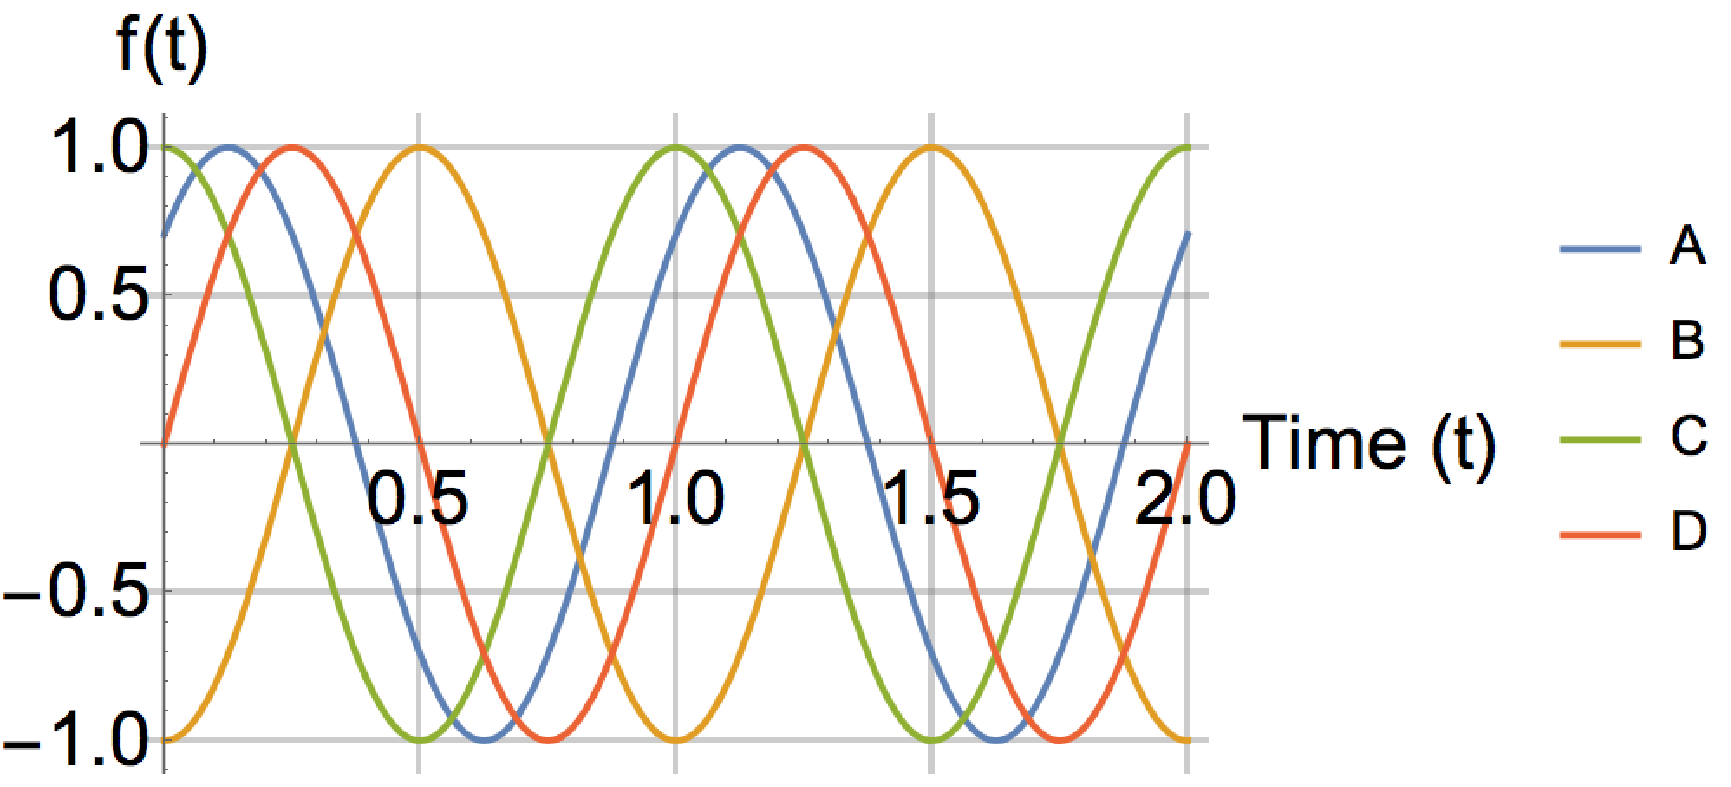
\includegraphics{phase_shift.png}

\subsection*{Solution}
\solstr{i}{5c0e8b}



%%%%%%%%%%%%%%%%%%%%%%%%%%%%%%%%%
\newpage
%%%%%%%%%%%%%%%%%%%%%%%%%%%%%%%%%
\section{Amplitude}

\subsection*{Comments}
Another important concept is amplitude. $\sin(2 \pi t)$ has an amplitude of 1, but this can be easily modified to go between $\pm A$ by multiplication with $A$.

\subsection*{Challenge}
The following 4 graphs correspond to the equation $A \sin(2 \pi k t)$ with variation in the values of $A$ and $k$. What is the sum of the values of $A$ for the following graphs? 

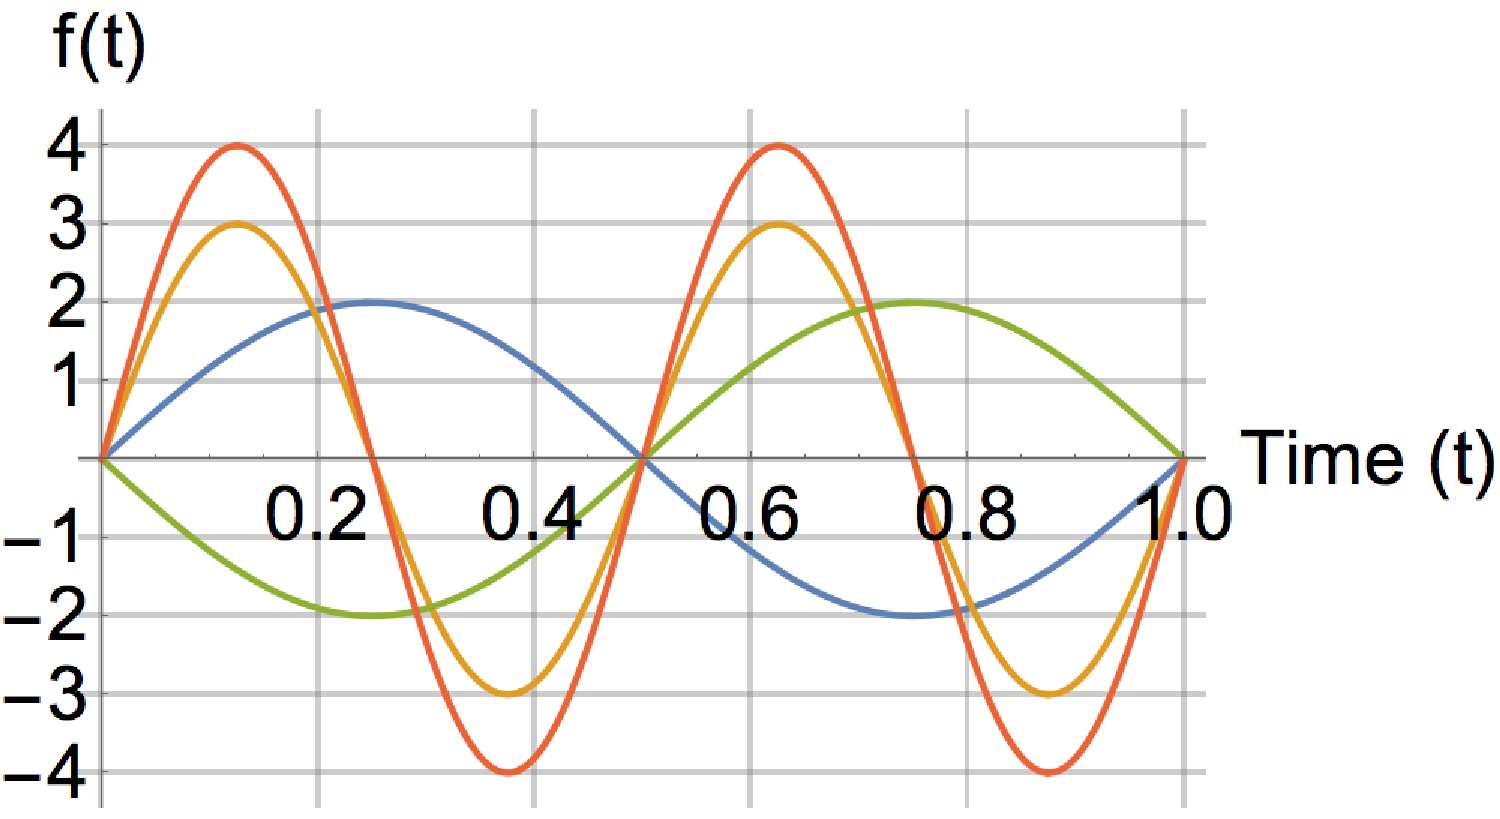
\includegraphics{amplitude.png}

\subsection*{Solution}
\solint{u}{6bce05}




%%%%%%%%%%%%%%%%%%%%%%%%%%%%%%%%%
\newpage
%%%%%%%%%%%%%%%%%%%%%%%%%%%%%%%%%
\section{Periodic and non-periodic signals}
\label{sec:periodic}

\subsection*{Resources}
\begin{itemize}
    \item Video: \url{https://www.youtube.com/watch?v=F_pdpbu8bgA}
    \item Book: 1.3 (\url{https://see.stanford.edu/materials/lsoftaee261/book-fall-07.pdf})
\end{itemize}

\subsection*{Challenge}
The list below contains periodic and non-periodic signals. Sum the points of the signals below that are \emph{periodic}.

1 point: $x(t) = t^2$\\
2 points: $x(t) = \sin(t)$\\
4 points: $x(t) = \sin(2 \pi t)$\\
8 points: $x(t) = \sin(2 \pi t + t)$\\
16 points: $x(t) = \sin(2 \pi t) + \sin(t)$\\
32 points: $x(t) = \sin(5 \pi t) + \sin(2 \pi t)$\\
64 points: $x(t) = \sin(5 \pi t) + \sin(37 \pi t)$\\
128 points: $x(t) = \sin(5 \pi t) + \sin(37.01 \pi t)$\\
256 points: $x(t) = \sin(5 \pi t) + \sin(\sqrt{2} \pi t)$\\
512 points: $x(t) = \sin(5 \sqrt{2} \pi t) + \sin(\sqrt{2} \pi t)$

\subsection*{Solution}
\solint{u}{5d906b}




%%%%%%%%%%%%%%%%%%%%%%%%%%%%%%%%%
\newpage
%%%%%%%%%%%%%%%%%%%%%%%%%%%%%%%%%
\section{Making non-periodic signals from periodic signals}

\subsection*{Challenge}
It is not immediately intuitive that it is possible to make a non-periodic signal by simply adding two periodic signals. Referring to the previous challenge, in no-more than 1 paragraph, explain how this is possible.

\subsection*{Solution}
Please compare your answer with your partner or ask the teacher in class.




%%%%%%%%%%%%%%%%%%%%%%%%%%%%%%%%%
\newpage
%%%%%%%%%%%%%%%%%%%%%%%%%%%%%%%%%
\section{Fundamental frequency}

\subsection*{Challenge}
Considering the periodic signals in challenge \ref{sec:periodic} in order of increasing point-score, calculate the fundamental frequency and period of the last periodic signal in the list.

\subsection*{Solution}
Frequency (Hz) (be careful about rounding up or down to 2 decimal places):\\
\soltwodp{a}{ac6698}

Period (s):\\
\soltwodp{b}{6fdff9}

%\chapter{Fourier Series}
%\section{Introduction to Fourier coefficients}
\label{sec:fouriercoeffintro}

\subsection*{Resources}
\begin{itemize}
    \item Book: 1.4 (\url{https://see.stanford.edu/materials/lsoftaee261/book-fall-07.pdf})
    \item Video: Lecture 2 (\url{https://www.youtube.com/watch?v=1rqJl7Rs6ps})
\end{itemize}

\subsection*{Challenge}
Deduce in a simple way the Fourier coefficients $a_1$ and $b_1$ in the Fourier series
\begin{equation}
    \sum_{k=1}^{N} a_k cos(2 \pi k t) + b_k sin(2 \pi k t)
\end{equation}

for a signal made up of multiple sine signals
\begin{equation}
    \sum_{k=1}^{N} A_k sin(2 \pi k t + \phi_k)
\end{equation}

for the following cases:
\begin{enumerate}
    \item $N=1$, $k=1$, $A_1=1$, $\phi_1=0$
    \item $N=1$, $k=1$, $A_1=1$, $\phi_1=\pi/2$
    \item $N=1$, $k=1$, $A_1=1$, $\phi_1=\pi/5$
\end{enumerate}

Hint: Using $sin(A+B) = sin(A) cos(B) + cos(A) sin(B)$ it should is possible to find the answer without resorting to complex calculation.

\subsection*{Solutions}
\begin{enumerate}
    \item MD5(o\_$a_k$) = a2c1fe\ldots, MD5(p\_$b_k$) = de80c6\ldots
    \item MD5(a\_$a_k$) = 718a6c\ldots, MD5(s\_$b_k$) = f86f0c\ldots
    \item MD5(d\_$a_k$) = 93d647\ldots, MD5(f\_$b_k$) = 9a7b58\ldots
\end{enumerate}

\timebox




%%%%%%%%%%%%%%%%%%%%%%%%%%%%%%%%%
\newpage
%%%%%%%%%%%%%%%%%%%%%%%%%%%%%%%%%

\section{Even and odd functions}

\subsection*{Resources}
\begin{itemize}
    \item Wikipedia: \url{https://en.wikipedia.org/wiki/Even_and_odd_functions}
\end{itemize}

\subsection*{Challenge}
Referring in part to the cases in challenge \ref{sec:fouriercoeffintro}, sum the points of all the following TRUE statements:

1 point: Case 1 is an odd function

2 points: Case 1 is an even function

4 points: Case 2 is an odd function

8 points: Case 2 is an even function

16 point: Case 3 is an odd function

32 points: Case 3 is an even function

64 points: $f(x)=Sin(x)$ is an odd function

128 points: $f(x)=Sin(x)$ is an even function

256 points: $f(x)=Cos(x)$ is an odd function

512 points: $f(x)=Cos(x)$ is an even function

1024 points: $f(x)=x$ is an odd function

2048 points: $f(x)=x$ is an even function

\subsection*{Solution}
X

\hash{g}{6a18c0}

\timebox




%%%%%%%%%%%%%%%%%%%%%%%%%%%%%%%%%
\newpage
%%%%%%%%%%%%%%%%%%%%%%%%%%%%%%%%%

\section{Fourier Coefficients of sin(x)}
\label{sec:fcsinx}

\subsection*{Resources}
\begin{itemize}
    \item Book: 1.4 (\url{https://see.stanford.edu/materials/lsoftaee261/book-fall-07.pdf})
    \item Video: Lecture 2 (\url{https://www.youtube.com/watch?v=1rqJl7Rs6ps})
\end{itemize}

\subsection*{Comments}
You should be able to follow the derivation of the formula for Fourier coefficients ($C_k$'s) in the video. Feel free to seek help if you have trouble.

\subsection*{Challenge}
By writing $sin(x)$ in exponential form, deduce the Fourier coefficients ($C_k$'s) for the function $sin(x)$, for the following cases:
\begin{enumerate}
    \item k = -1
    \item k = 0
    \item k = 1
\end{enumerate}

\subsection*{Solutions}
\subsubsection{k=-1}
X

\hash{h}{28f251}

\subsubsection{k=0}
X

\hash{j}{4fd3f6}

\subsubsection{k=1}
X

\hash{k}{e82a2a}

\timebox




%%%%%%%%%%%%%%%%%%%%%%%%%%%%%%%%%
\newpage
%%%%%%%%%%%%%%%%%%%%%%%%%%%%%%%%%

\section{Fourier Coefficients of 1 + sin(x)}

\subsection*{Resources}
\begin{itemize}
    \item Book: 1.4 (\url{https://see.stanford.edu/materials/lsoftaee261/book-fall-07.pdf})
    \item Video: Lecture 2 (\url{https://www.youtube.com/watch?v=1rqJl7Rs6ps})
\end{itemize}

\subsection*{Comments}
You should be able to follow the derivation of the formula for Fourier coefficients in the video. Feel free to seek help if you have trouble.

\subsection*{Challenge}
Continuing from challenge \ref{sec:fcsinx}, deduce the Fourier coefficients ($C_k$'s) for the function $1+sin(x)$, for the following cases:
\begin{enumerate}
    \item k = -1
    \item k = 0
    \item k = 1
\end{enumerate}

\subsection*{Solutions}
\subsubsection{k=-1}
X

\hash{z}{39e026}

\subsubsection{k=0}
X

\hash{x}{0ef183}

\subsubsection{k=1}
X

\hash{c}{89b992}

\timebox




%%%%%%%%%%%%%%%%%%%%%%%%%%%%%%%%%
\newpage
%%%%%%%%%%%%%%%%%%%%%%%%%%%%%%%%%

\section{Relation of positive and negative Fourier coefficients for a real signal}

\subsection*{Resources}
\begin{itemize}
    \item Book: 1.4 (\url{https://see.stanford.edu/materials/lsoftaee261/book-fall-07.pdf})
    \item Video: Lecture 2 (\url{https://www.youtube.com/watch?v=1rqJl7Rs6ps})
\end{itemize}

\subsection*{Challenge}
If the Fourier coefficient $C_1$ is $4 + 6i$, what is the Fourier coefficient $C_{-1}$?

\subsection*{Solution}
X

\hash{m}{36ab38}

\timebox




%%%%%%%%%%%%%%%%%%%%%%%%%%%%%%%%%
\newpage
%%%%%%%%%%%%%%%%%%%%%%%%%%%%%%%%%

\section{Converting between trigonometric and exponential forms}
\label{sec:trigexpconvert}

\subsection*{Resources}
\begin{itemize}
    \item Book: 1.4 (\url{https://see.stanford.edu/materials/lsoftaee261/book-fall-07.pdf})
    \item Video: Lecture 2 (\url{https://www.youtube.com/watch?v=1rqJl7Rs6ps})
\end{itemize}

\subsection*{Challenge}
Derive an expression for $C_k$ in terms of the $a_k$'s and $b_k$'s in the expression
\begin{equation}
    f(t) = \frac{a_0}{2} + \sum_{k=1}^{k=N} a_k cos(2 \pi k t) + b_k sin(2 \pi k t) = \sum_{k=-N}^{k=N} C_k e^{2 \pi i k t}
\end{equation}

To check your answer, substitute $a_0 = 1$, $a_1 = 3$ and $b_1 = 5$ as required to calculate $C_k$ for k = -1, 0 and 1.

\subsection*{Solutions}
\subsubsection{k=-1}
X

\hash{v}{052df3}

\subsubsection{k=0}
X

\hash{b}{fb29ff}

\subsubsection{k=1}
X

\hash{n}{284b53}

\timebox




%%%%%%%%%%%%%%%%%%%%%%%%%%%%%%%%%
\newpage
%%%%%%%%%%%%%%%%%%%%%%%%%%%%%%%%%

\section{The Fourier series of $f(t)=t$: $C_0$}

\subsection*{Resources}
\begin{itemize}
    \item Book: 1.5, 1.7 (\url{https://see.stanford.edu/materials/lsoftaee261/book-fall-07.pdf})
    \item Video: Lecture 3 (\url{https://www.youtube.com/watch?v=BjBb5IlrNsQ})
\end{itemize}

\subsection*{Challenge}
Considering the function $f(t)=t$ over the interval 0 to 1, calculate the Fourier coefficient $C_0$ using the derived formula for Fourier coefficients. Compare with the average over the interval.

\subsection*{Solution}
X

\hash{aa}{2708ad}

\timebox




%%%%%%%%%%%%%%%%%%%%%%%%%%%%%%%%%
\newpage
%%%%%%%%%%%%%%%%%%%%%%%%%%%%%%%%%

\section{The Fourier series of $f(t)=t$: $C_k$}

\subsection*{Resources}
\begin{itemize}
    \item Book: 1.5, 1.7 (\url{https://see.stanford.edu/materials/lsoftaee261/book-fall-07.pdf})
    \item Video: Lecture 3 (\url{https://www.youtube.com/watch?v=BjBb5IlrNsQ})
\end{itemize}

\subsection*{Challenge}
Considering the function $f(t)=t$, calculate a general expression for the Fourier coefficients $C_k$ where $k \ne 0$.

To check your answer, evaluate the Fourier coefficient for $k=-30$.

\subsection*{Solution}
X

\hash{bb}{e904e9}

\timebox




%%%%%%%%%%%%%%%%%%%%%%%%%%%%%%%%%
\newpage
%%%%%%%%%%%%%%%%%%%%%%%%%%%%%%%%%

\section{The Fourier series of $f(t)=t$ in exponential form}
\label{sec:fstexpform}

\subsection*{Resources}
\begin{itemize}
    \item Book: 1.4 (\url{https://see.stanford.edu/materials/lsoftaee261/book-fall-07.pdf})
    \item Video: Lecture 3 (\url{https://www.youtube.com/watch?v=BjBb5IlrNsQ})
\end{itemize}

\subsection*{Challenge}
Write the function $f(t)=t$ in terms of its infinite exponential Fourier series.

To check your answer, evaluate the Fourier series up to $n=2$ with $t=0.8$.

The graph with increasing values of $n$ looks like this:

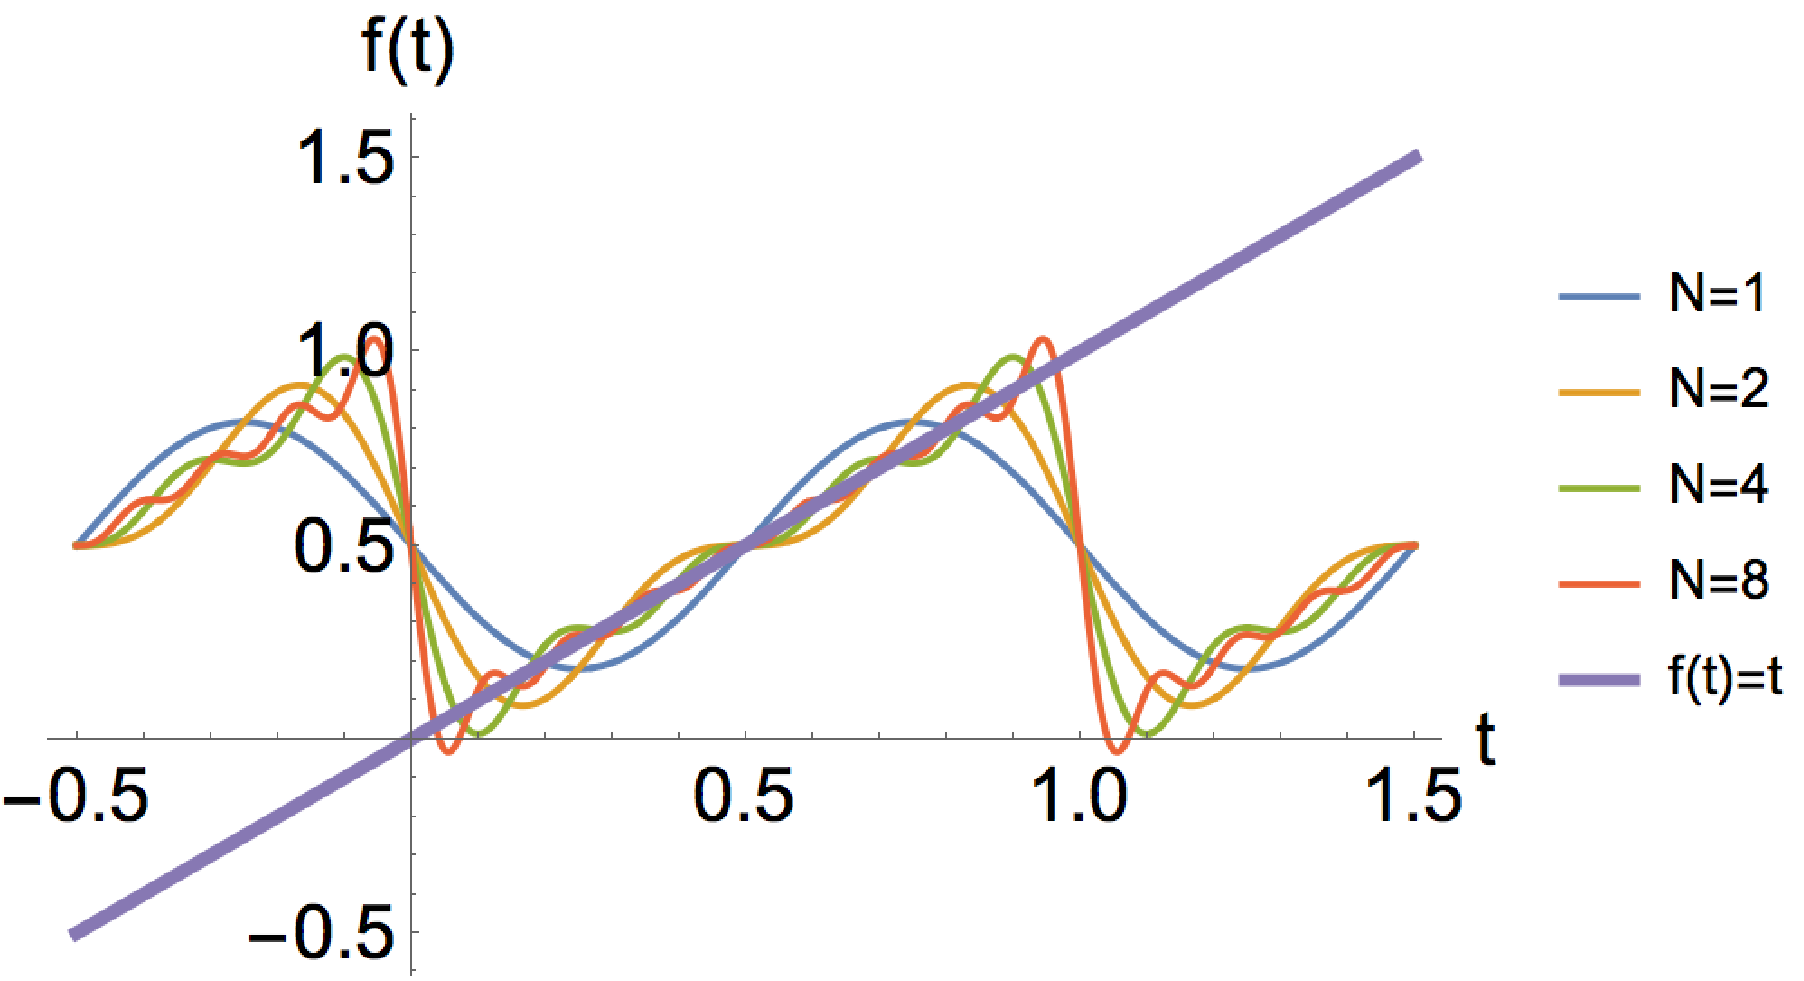
\includegraphics{fourier_series_t.png}

\subsection*{Solution}
X

\hash{cc}{d21e19}

\timebox




%%%%%%%%%%%%%%%%%%%%%%%%%%%%%%%%%
\newpage
%%%%%%%%%%%%%%%%%%%%%%%%%%%%%%%%%

\section{The Fourier series of $f(t)=t$ in trigonometric form}

\subsection*{Resources}
\begin{itemize}
    \item Book: 1.5, 1.7 (\url{https://see.stanford.edu/materials/lsoftaee261/book-fall-07.pdf})
    \item Video: Lecture 2 (\url{https://www.youtube.com/watch?v=1rqJl7Rs6ps})
\end{itemize}

\subsection*{Comment}
Many textbooks will work in terms of ``Fourier sine series'' and ``Fourier cosine series''. For a function that is perfectly even or odd, it is possible to write a Fourier series using one of these two forms. There are direct approaches to calculating sine and cosine Fourier series, in contrast to the route taken here via the exponential form. We will continue to work in the exponential form however, since not only does this provide a deeper understanding, but you can always easily switch between exponential and trigonometric forms if you really want to.


\subsection*{Challenge}
Re-write the series obtained in challenge \ref{sec:fstexpform} in terms of a trigonometric infinite series (ie, using sines and cosines).

To check your answer, evaluate the Fourier series up to $n=2$ with $t=0.8$ and ensure that you get the same answer as you did for challenge \ref{sec:fstexpform}.

\timebox




%%%%%%%%%%%%%%%%%%%%%%%%%%%%%%%%%
\newpage
%%%%%%%%%%%%%%%%%%%%%%%%%%%%%%%%%
\section{Periods other than unity}

\subsection*{Resources}
\begin{itemize}
    \item Book: 1.6 (\url{https://see.stanford.edu/materials/lsoftaee261/book-fall-07.pdf})
\end{itemize}

\subsection*{Challenge}
Determine the Fourier series for the same function as in \ref{sec:fstexpform} ($f(t)=t$), except approximate the function over the region $1<x<3$ instead of $0<x<1$.

To check your answer, evaluate the Fourier series up to $n=2$ with $t=1.8$.

The graph with increasing values of $n$ looks like this:

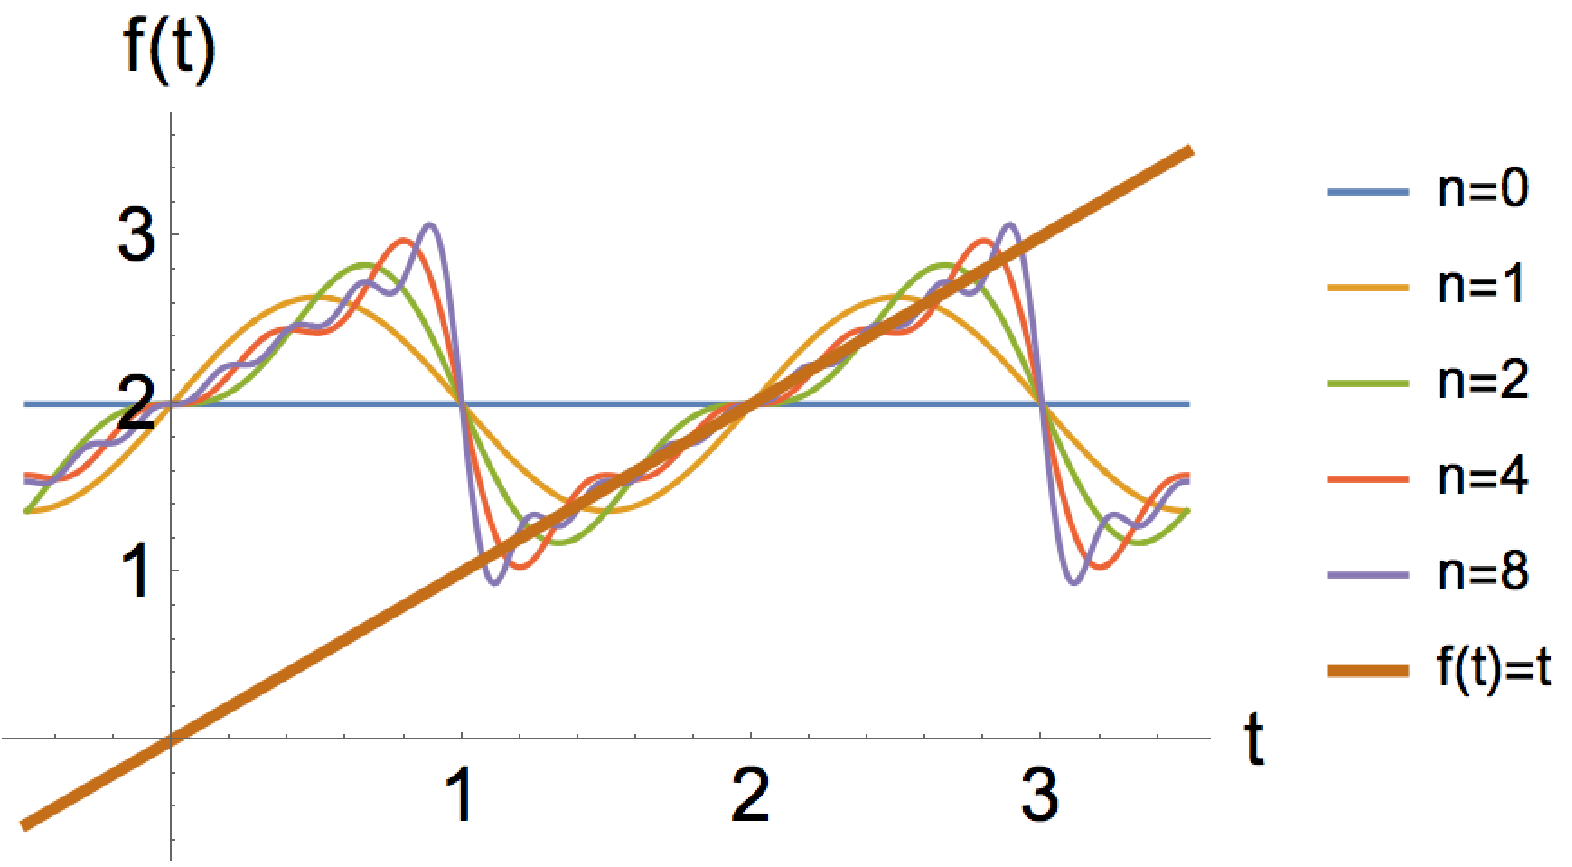
\includegraphics{fs_other_periods.png}

\subsection*{Solution}
X

\hash{dd}{83e943}

\timebox




%%%%%%%%%%%%%%%%%%%%%%%%%%%%%%%%%
\newpage
%%%%%%%%%%%%%%%%%%%%%%%%%%%%%%%%%
\section{Infinite series}

\subsection*{Comment}
It is important to understand why some series are infinite, while others are not (well, technically all series are infinite since they all involve sums to $n=\infty$, however for some series the Fourier coefficients are all zero above a certain value of $n$). Therefore, make sure you understand why the answer is as it is, below. If you don't, be sure to discuss with others.

\subsection*{Challenge}
The Fourier series is a sum to $\pm \infty$, however in some cases the coefficients ($C_k$'s) are zero beyond a certain number of terms. Which of the terms below will have Fourier coefficients that are all zero after a certain number of terms? Sum the points of these functions.

1 point: $x$

2 points: $x^2$

4 points: $cos(2 x) + 3 sin(7 x)$

8 points: $e^{2 \pi i x}$

\subsection*{Solution}
X

\hash{ee}{8e05a4}

\timebox




%%%%%%%%%%%%%%%%%%%%%%%%%%%%%%%%%
\newpage
%%%%%%%%%%%%%%%%%%%%%%%%%%%%%%%%%
\section{k-symmetry}

\subsection*{Challenge}
Determine what X and Y represent algebraically.
\begin{equation}
    cos(k \pi t) = \frac{1}{2} e^{-k i\pi t} + \frac{1}{2} e^{\bm{X} i \pi x}
\end{equation}
\begin{equation}
    sin(k \pi t) = \frac{1}{2} i e^{\bm{Y} i \pi t} - \frac{1}{2} i e^{k i \pi t}
\end{equation}

To check your answers you may substitute any appropriate values from the following list: $k=2$, $t=1$

\subsection*{Solution}
X

\hash{ff}{942d6f}

Y

MD5(gg\_Y) = a379b8\ldots

\timebox




%%%%%%%%%%%%%%%%%%%%%%%%%%%%%%%%%
\newpage
%%%%%%%%%%%%%%%%%%%%%%%%%%%%%%%%%
\section{Direct trigonometric calculation of a Fourier series: the coefficients}
\label{sec:fs_squarewave}

\section*{Comment}
This challenge introduces several key concepts at once, including decoupling of integral intervals and periodicity, the concept of a square wave and direct trigonometric evaluation of Fourier series. If you can master this you'll be in a really strong position.

It is hopefully clear now that for real signals, due to the symmetry of the positive and negative k's, one can fully compose Fourier series in terms of sine and cosine. In challenge \ref{sec:trigexpconvert} we saw the formula for the function in terms of Fourier coefficients $a_0$, $a_n$ and $b_n$. While we will not use this approach, it is important to be able to utilise such a formulation since this is the way some books present it and some people have learnt it. Therefore, without proof, the coefficients can be calculated using

\begin{equation}
    a_k = \frac{2}{T} \int_{t_0}^{t_0+T} f(t) Cos(2 \pi k t/T)
\end{equation}
\begin{equation}
    b_k = \frac{2}{T} \int_{t_0}^{t_0+T} f(t) Sin(2 \pi k t/T)
\end{equation}

\subsection*{Challenge}
Using the direct trigonometric Fourier series, obtain a general expression for the $a_k$ and $b_k$ coefficients for the square-wave signal with periodicity 4

\begin{equation}
    f(t)=
    \begin{cases}
        1 & \text{for } -1<t<1 \\
        0 & \text{for } 1<t<3
    \end{cases}
\end{equation}

A graph of the function, including the solution for various values of $n$, is shown here:

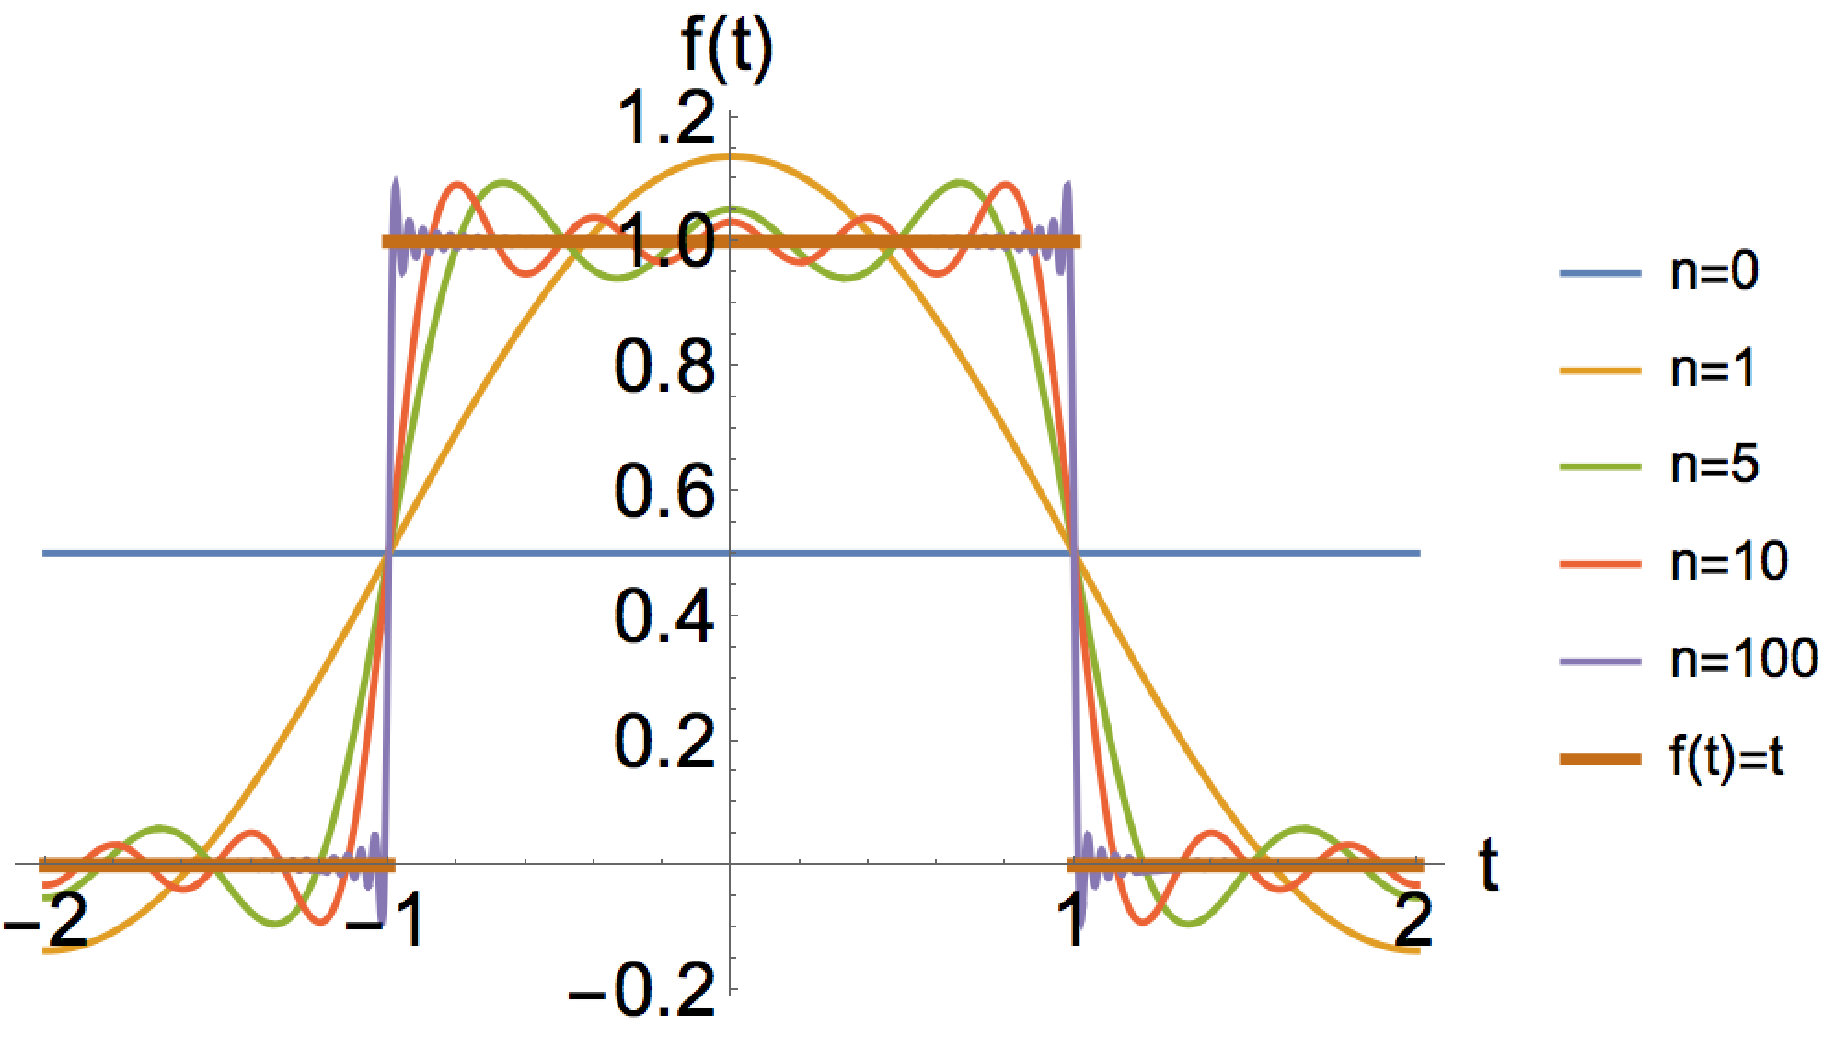
\includegraphics{fs_square_wave.png}

Note the symmetry of the problem. Can you see what terms will be zero? To check your solution, calculate $a_k$ and $b_k$ for $k=0$, $k=2$ and $k=3$. Also note that you will have to break the integrals into two parts and sum them in order to tackle this problem.

\subsection*{Solution}
\begin{tabular}{|l|l|l|}
    \hline
    $k$ & $a_k$ & $b_k$ \\
    \hline
    0 & MD5(hh\_X)=e57c15\ldots & MD5(ii\_X)=377fe2\ldots \\
    2 & MD5(jj\_X)=54aaa1\ldots & MD5(kk\_X)=be063f\ldots \\
    3 & MD5(mm\_X)=b8fce7\ldots & MD5(nn\_X)=b6fbaf\ldots \\
    \hline
\end{tabular}

\timebox




%%%%%%%%%%%%%%%%%%%%%%%%%%%%%%%%%
\newpage
%%%%%%%%%%%%%%%%%%%%%%%%%%%%%%%%%
\section{Direct trigonometric calculation of a Fourier series: the series}

\subsection*{Challenge}
Calculate the Fourier series for the square wave introduced in challenge \ref{sec:fs_squarewave} using direct trigonometric calculation for up to $n=3$. Check your solution by evaluating for $t=0.1$.

\subsection*{Solution}
\six{}

\hash{oo}{bd7e5e}

\timebox




%%%%%%%%%%%%%%%%%%%%%%%%%%%%%%%%%
\newpage
%%%%%%%%%%%%%%%%%%%%%%%%%%%%%%%%%
\section{2D orthogonal vectors}

\subsection*{Resources}
\begin{itemize}
    \item Book: 1.9 (\url{https://see.stanford.edu/materials/lsoftaee261/book-fall-07.pdf})
\end{itemize}

\subsection*{Challenge}
Sum the points of the vectors in 2D that are orthogonal:

1 point: (5, 4) and (-1, 1.25)

2 points:  (2, -3) and (-6, 4)

4 points: (-2.25, 1.5) and (2, 3)

8 points: (4.5, 4) and (3, -3.375)

16 points: (6, 4) and (4, -6)

32 points: (5, 1) and (-2, 8.125)

64 points: (0, 1) and (1, 0)

128 points: (1, 1) and (1, 1)

\subsection*{Solution}
\six{}

\hash{pp}{92843f}

\timebox




%%%%%%%%%%%%%%%%%%%%%%%%%%%%%%%%%
\newpage
%%%%%%%%%%%%%%%%%%%%%%%%%%%%%%%%%
\section{Orthonormal basis}

\subsection*{Resources}
\begin{itemize}
    \item Video: \url{https://www.khanacademy.org/math/linear-algebra/alternate-bases/orthonormal-basis/v/linear-algebra-introduction-to-orthonormal-bases}
\end{itemize}

\subsection*{Challenge}
Sum the points of the following vectors that form an orthonormal basis:

1 point :
($\displaystyle \frac{1}{\sqrt{5}}, \frac{2}{\sqrt{5}}$) and
($\displaystyle \frac{2}{\sqrt{5}}, \frac{4}{\sqrt{5}}$)

2 points:
($\displaystyle \frac{2}{\sqrt{5}}$, $\displaystyle \frac{1}{\sqrt{5}}$) and
($\displaystyle \frac{-1}{\sqrt{5}}$, $\displaystyle \frac{2}{\sqrt{5}}$)

4 points:
($\displaystyle \frac{2}{\sqrt{2}}, \sqrt{\frac{7}{8}}, \frac{1}{\sqrt{6}}$),
($\displaystyle -\sqrt{\frac{2}{5}}, \frac{7}{\sqrt{14}}, -\frac{1}{\sqrt{6}}$) and
($\displaystyle \frac{1}{\sqrt{3}},  \frac{1}{5 \sqrt{3}}, -\frac{7}{5 \sqrt{3}}$)

8 points:
($\displaystyle \frac{1}{\sqrt{21}}, \frac{2}{\sqrt{21}}, \frac{4}{\sqrt{21}}$),
($\displaystyle -\sqrt{\frac{2}{7}}, \frac{3}{\sqrt{14}}, -\frac{1}{\sqrt{14}}$) and
($\displaystyle \sqrt{\frac{2}{3}},  \frac{1}{\sqrt{6}}, -\frac{1}{\sqrt{6}}$)

16 points:
($\displaystyle \frac{1}{\sqrt{6}}, \sqrt{\frac{2}{3}}, \frac{1}{\sqrt{6}}$),
($\displaystyle -\frac{1}{\sqrt{2}},  \frac{2 \sqrt{2}}{5}, -\frac{3}{5 \sqrt{2}}$) and
($\displaystyle \frac{1}{\sqrt{3}},  \frac{1}{5 \sqrt{3}}, -\frac{7}{5 \sqrt{3}}$)

32 points:
($0, 2$) and ($2, 0$)

64 points:
($0, 1$) and ($1, 0$)

\subsection*{Solution}
\six{}

\hash{qq}{097fd7}

\timebox




%%%%%%%%%%%%%%%%%%%%%%%%%%%%%%%%%
\newpage
%%%%%%%%%%%%%%%%%%%%%%%%%%%%%%%%%
\section{Natural basis}

\subsection*{Resources}
\begin{itemize}
    \item Book: 1.9 (\url{https://see.stanford.edu/materials/lsoftaee261/book-fall-07.pdf})
\end{itemize}

\subsection*{Challenge}
Sum the components of the following vectors of an orthonormal basis in $\mathbb{R}^{300}$ space:

\begin{itemize}
    \item First component of the first vector
    \item first component of the second vector
    \item 200th component of the 100th vector
    \item 200th component of the 200th vector
    \item last component of the 299th vector
    \item last component of the last vector
\end{itemize}

\subsection*{Solution}
\six{}

\hash{rr}{095c77}

\timebox




%%%%%%%%%%%%%%%%%%%%%%%%%%%%%%%%%
\newpage
%%%%%%%%%%%%%%%%%%%%%%%%%%%%%%%%%
\section{Orthonormal basis for Fourier series}

\subsection*{Resources}
\begin{itemize}
    \item Book: 1.9 (\url{https://see.stanford.edu/materials/lsoftaee261/book-fall-07.pdf})
\end{itemize}

\subsection*{Comment}
The previous challenges have focussed on the orthogonality and orthonormality of vectors. We now make the jump to functions. As chapter 1.9 explains, although its not perfect, the analogy between vectors and functions is a good way to help understand and visualise the role that the terms of a Fourier series play in defining a basis upon which to describe a function.

\subsection*{Challenge}
Starting from the inner product of two terms ($e^{2 \pi i k_1 t}$, $e^{2 \pi i k_2 t}$) of a Fourier series, demonstrate that the terms of a Fourier series form an orthonormal basis. \textbf{Show a full derivation}.

To check your intuition, you may evaluate the following cases:

$X = (e^{2 \pi i k_1 t}, e^{2 \pi i k_1 t})$

$Y = (e^{2 \pi i k_1 t}, e^{2 \pi i k_2 t})$

\subsection*{Solution}
If you are not confident about your derivation, please check with someone else. If there is any step that you do not fully understand, do not hesitate to ask. If you do not understand the connection between previous challenges on vectors and this challenge using functions, do not hesitate to ask someone.

\textbf{X}

\hash{ss}{8f7f41}

\textbf{Y}

MD5(tt\_Y) = 2c669b\ldots

\timebox




%%%%%%%%%%%%%%%%%%%%%%%%%%%%%%%%%
\newpage
%%%%%%%%%%%%%%%%%%%%%%%%%%%%%%%%%
\section{Circles and Fourier series}

\subsection*{Resources}
\begin{itemize}
    \item Video 1: \url{https://www.youtube.com/watch?v=Y9pYHDSxc7g}
    \item Video 2: \url{https://www.youtube.com/watch?v=LznjC4Lo7lE}
\end{itemize}

\subsection*{Comment}
In the first lecture we saw how it was possible to approximate any function given enough circles. Here we link what you have learned back to that first lecture. I strongly recommend viewing the fun and informative videos listed here under Resources. In summary, by building a Fourier series you are representing a function using an orthonormal basis, where each component of the basis can be considered visually as a circle operating with individual radius and frequency on the real-imaginary plane. If, after completing this challenge, that last sentence makes sense to you, then you have achieved the first major goal of this course.

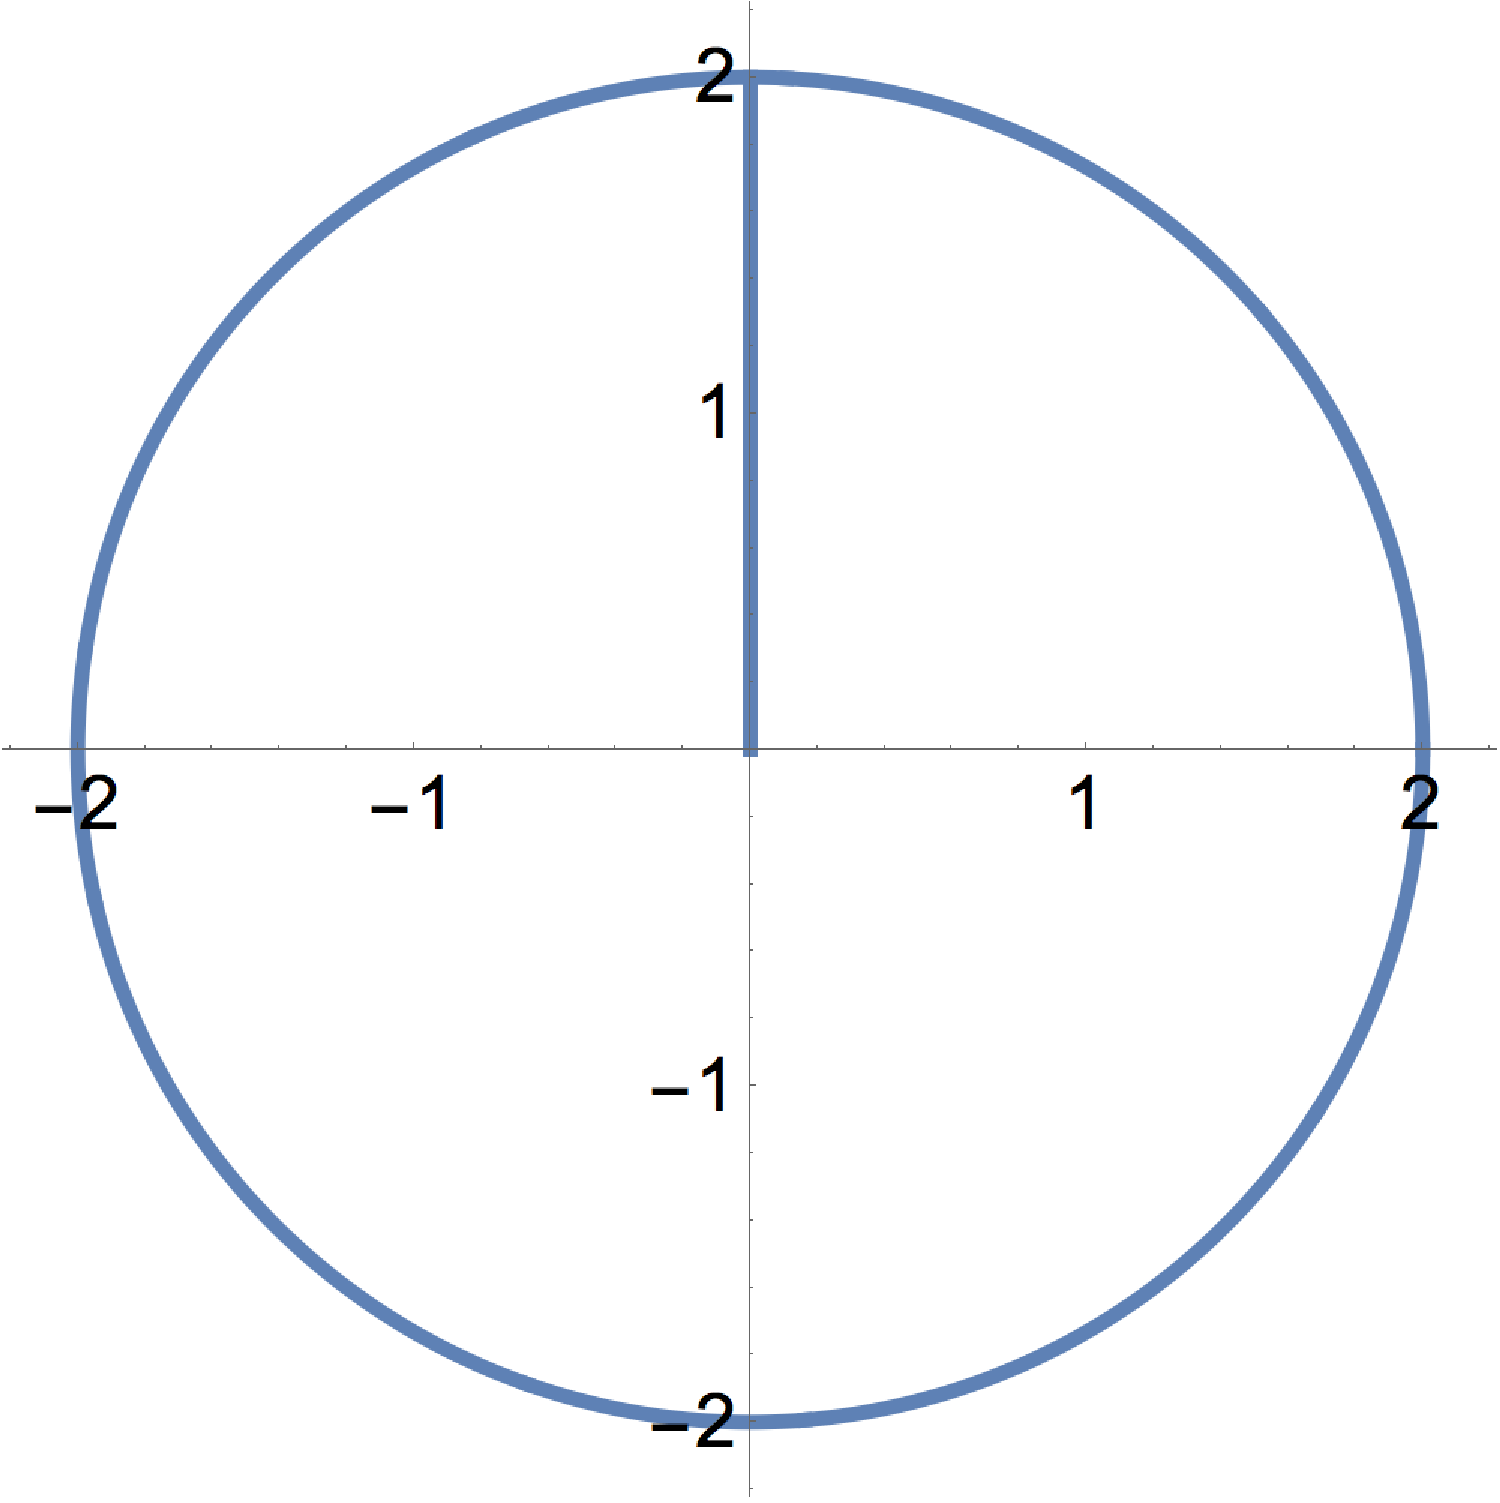
\includegraphics[scale=0.5]{circle.png}

\subsection*{Challenge}
Treating the x-axis as the real axis and the y-axis as the imaginary axis, arrange the equations below in the following order:

\begin{enumerate}
    \item A point moving round on a circle with radius 2 units and frequency 2 Hz
    \item A point moving round on a circle with radius 3 units and frequency 1 Hz
    \item A point moving round on a circle with radius 2 units and a period of 1 second
    \item A point moving round on a circle with radius 3 units and a period of 2 seconds
\end{enumerate}

Equations:

$\displaystyle A e^{2 \pi i k t}$ where $t$ is time in seconds and the values of $A$ and $k$ are as follows:

A: $A=2$, $k=2$ 

B: $A=3$, $k=1$

C: $A=3$, $k=0.5$

D: $A=2$, $k=1$

\subsection*{Solution}
\six{}

\hash{uu}{cb7845}

\timebox

% Convergence?
% Gibbs phenomena?



%\chapter{Fourier Transform}
%% Make clear about using the window function in the frequency domain as a filter.
%%%%%%%%%%%%%%%%%%%%%%%%%%%%%%%%%
\newpage
%%%%%%%%%%%%%%%%%%%%%%%%%%%%%%%%%
\section{The transition to the Fourier Transform}

\subsection*{Resources}
\begin{itemize}
    \item Video I: Lecture 5 from 27:00 (\url{https://youtu.be/X5qRpgfQld4?t=27m})
    \item Video II: Lecture 6 up to 20:00 (\url{https://www.youtube.com/watch?v=4lcvROAtN_Q})
    \item Book: Chapter 2 (\url{https://see.stanford.edu/materials/lsoftaee261/book-fall-07.pdf})
\end{itemize}

\subsection*{Comment}
Until now we have been considering Fourier series. This is however limited to describing periodic phenomena since it is assumed that the signal repeats outside the region of integration. The Fourier transform can be thought of as an extension of Fourier series which allows the analysis of non-periodic phenomena.

The suggested resources provide an excellent intuitive path of the connection between Fourier series and Fourier transforms, and this challenge is designed to give you the opportunity to take some time to try to understand the main concepts behind the transition.

\subsection*{Challenge}
Using the resources above, describe how to make the transition from Fourier series to the Fourier transform.



%%%%%%%%%%%%%%%%%%%%%%%%%%%%%%%%%
\newpage
%%%%%%%%%%%%%%%%%%%%%%%%%%%%%%%%%
\section{Fourier transform notation}

\subsection*{Comment}
Just so that you are aware, you should know that there are various equivalent notations in use, and if you use the Fourier transform in your later career you will probably come across notations different to the ones used in this course. This is partly because Fourier analysis is applicable to a wide range of fields and each field tends to have its own conventions based on how the Fourier transform is interpreted physically (if at all) in that field.

In general, the Fourier transform is given by
\begin{equation}
    \mathcal{F}f(\omega) = \sqrt{\frac{|b|}{(2 \pi)^{1-a}}} \int_{-\infty}^{\infty} f(t) e^{i b \omega t} dt
\end{equation}

where $a$ and $b$ typically take on values such as 

\begin{tabular}{|c|c c|}
    \hline
    \textbf{Case} & \textbf{a} & \textbf{b} \\
    \hline
    \textbf{1}    & 0          & 1          \\
    \textbf{2}    & 1          & -1         \\
    \textbf{3}    & -1         & 1          \\
    \textbf{4}    & 0          & -2$\pi$   \\
    \hline
\end{tabular}

\subsection*{Challenge}
1. Write the Fourier transform using the four possible notations.

2. Add the points of the legitimate forms of Fourier notation:

1 point: $\displaystyle \mathcal{F}f(w)=\frac{1}{\sqrt{2 \pi}} \int_{-\infty}^{\infty} e^{i w t} f(t) dt$

2 points: $\displaystyle \mathcal{F}f(w)=\int_{-\infty}^{\infty} e^{-i 2 \pi w t} f(t) dt$

4 points: $\displaystyle \mathcal{F}f(w)=\frac{1}{2 \pi} \int_{-\infty}^{\infty} e^{i w t} f(t) dt$

8 points: $\displaystyle \mathcal{F}f(s)=\frac{1}{\sqrt{2 \pi}} \int_{-\infty}^{\infty} e^{i \pi s t} f(t) dt$

16 points: $\displaystyle \mathcal{F}f(w)=\int_{-\infty}^{\infty} e^{i 2 \pi w t} f(t) dt$

32 points: $\displaystyle \mathcal{F}f(s)=\int_{-\infty}^{\infty} e^{-i s t} f(t) dt$

\subsection*{Solution}
2.\\
\solint{c}{8cecbb}




%%%%%%%%%%%%%%%%%%%%%%%%%%%%%%%%%
\newpage
%%%%%%%%%%%%%%%%%%%%%%%%%%%%%%%%%
\section{L'H\^opital's rule}

\subsection*{Challenge}
Use L'H\^opital's rule to determine the limit of
\begin{equation}
    \frac{\sin(x)}{x}
\end{equation}
as $x \rightarrow 0$.

\subsection*{Solution}
\solint{d}{9948c6}




%%%%%%%%%%%%%%%%%%%%%%%%%%%%%%%%%
\newpage
%%%%%%%%%%%%%%%%%%%%%%%%%%%%%%%%%
\section{Fourier transform of a window function}
\label{sec:tophat}

\subsection*{Resources}
\begin{itemize}
    \item Book: Chapter 2.1 (\url{https://see.stanford.edu/materials/lsoftaee261/book-fall-07.pdf}) %, page 68, particularly at the bottom of the page
    \item Video: Lecture 6 starting from 29:26 (\url{https://youtu.be/4lcvROAtN_Q?t=29m26s})
\end{itemize}

\subsection*{Challenge}
Calculate the Fourier Transform for the window function

\begin{equation}
    f(t)=
    \begin{cases}
        1 & \text{for } |t| < 1/2 \\
        0 & \text{for } |t| > 1/2
    \end{cases}
\end{equation}

In graph-form the function and its transform appear as follows:

\begin{tabular}{cc}
    \textbf{Function} & \textbf{Fourier transform} \\
    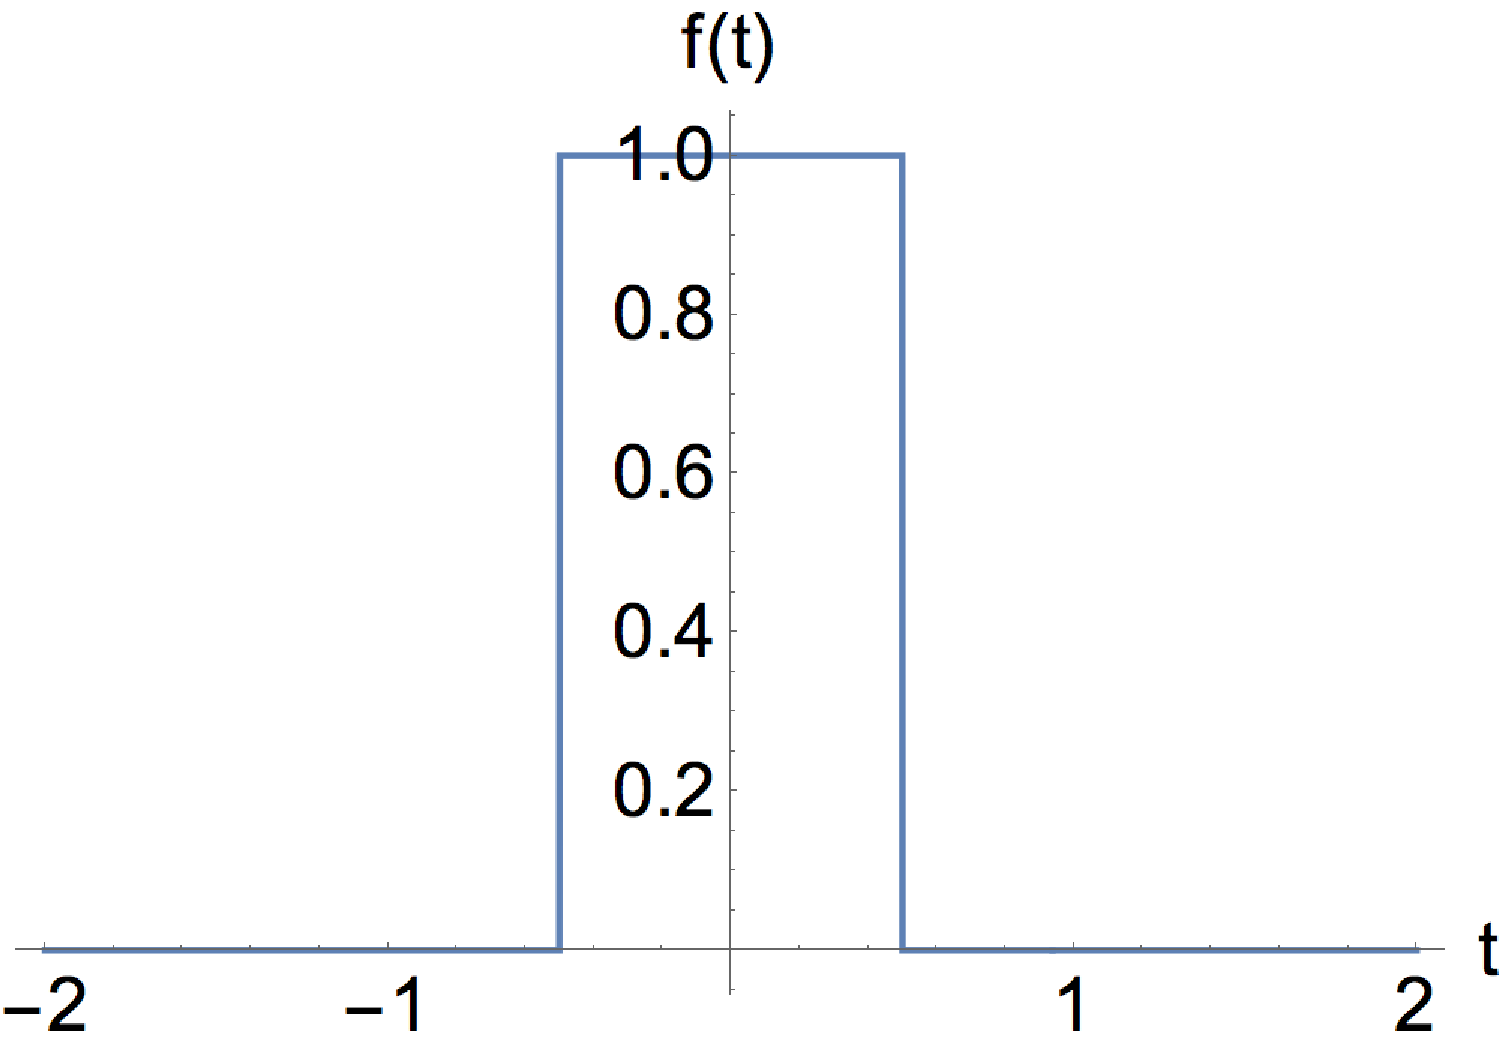
\includegraphics[scale=0.5]{window1.png} & 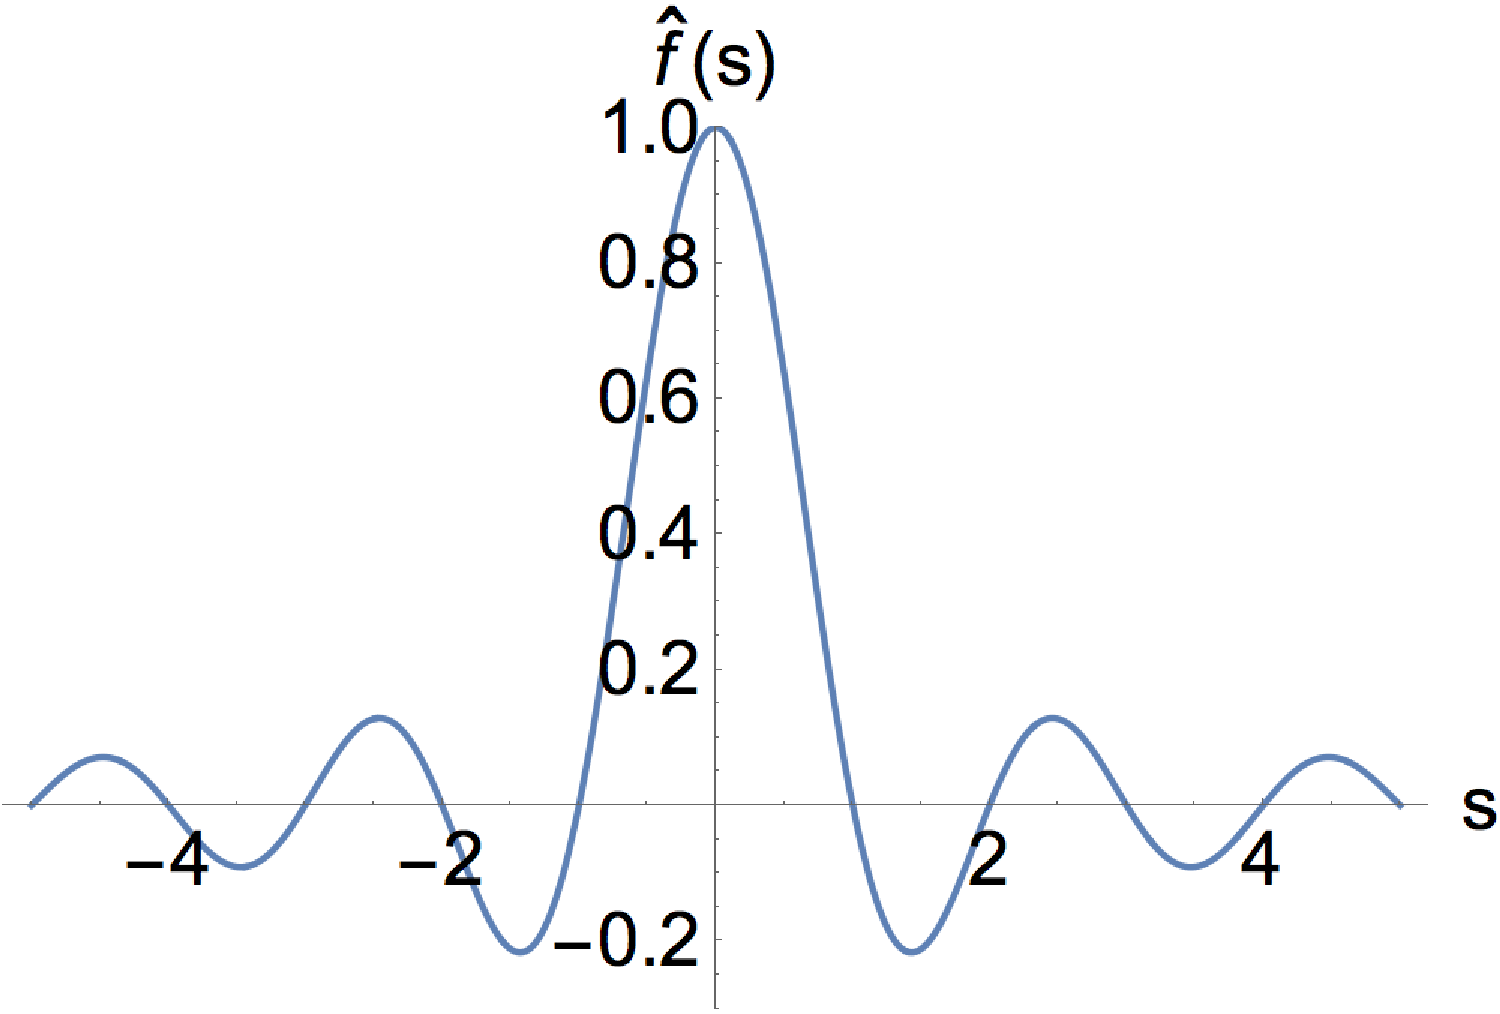
\includegraphics[scale=0.5]{window1ft.png}
\end{tabular}

\subsection*{Solution}
You should find that your solution is consistent with $\hat{f}(s=1.5)=-0.21$.




%%%%%%%%%%%%%%%%%%%%%%%%%%%%%%%%%
\newpage
%%%%%%%%%%%%%%%%%%%%%%%%%%%%%%%%%
\section{Fourier transform of sine and cosine}

\subsection*{Comments}
With Fourier series we understood the integer $k$ in $\sin(2 \pi k t)$ as the frequency of the signal, and by building up the sum of sines and cosines (using exponential notation) we could reproduce very well an arbitrary periodic signal. In the case of challenges \ref{sec:fcsinx} and \ref{sec:fcsinxp1} we determined the Fourier coefficients for a single-frequency $k=1$ sine signal.

Can we still understand the $s$ in the Fourier transform $\int_{-\infty}^{\infty} f(t) e^{i 2 \pi s t}$ as analogous to $k$ somehow? What happens when you take the Fourier transform of a single-frequency signal? How is phase-information encoded? This is difficult to visualise but this challenge, dealing with simple single-frequency signals, should give you an initial insight.

\subsection*{Challenge}
1. Calculate the Fourier transforms of\\
(I) $\sin(2 \pi t)$\\
(II) $\cos(2 \pi t)$

You may find the following identity useful:
\begin{equation}
    \int_{-\infty}^{\infty} e^{-i 2 \pi (s+c) t} = \delta(s+c)
\end{equation}

2. Write $\sin(2 \pi t)$ and $\cos(2 \pi t)$ in terms of complex exponentials. Can you see an analogy between the Fourier transforms you calculated and the complex exponential forms of sine and cosine?

\subsection*{Solution}
1. In both cases, to check your answers calculate $\int_0^2 f(s) ds$.

(I)\\
\solimagtwodp{e}{923c59}

(II)\\
\solimagtwodp{f}{c68bbf}

2. Please discuss with your partner in class, and ask the teacher if you are unsure.



%%%%%%%%%%%%%%%%%%%%%%%%%%%%%%%%%
\newpage
%%%%%%%%%%%%%%%%%%%%%%%%%%%%%%%%%
\section{Fourier transform of a triangle function}
\label{sec:ft_triangle}

\subsection*{Resources}
\begin{itemize}
    \item Book: Chapter 2.2.1 (\url{https://see.stanford.edu/materials/lsoftaee261/book-fall-07.pdf})
    \item Video: Lecture 6 (\url{https://www.youtube.com/watch?v=4lcvROAtN_Q})
\end{itemize}

\subsection*{Challenge}
What is the Fourier transform of a triangle function, as shown below, in terms of the window function of challenge \ref{sec:tophat}? You may just state the function; calculation is not required unless you would like to try and prove it.

\begin{tabular}{cc}
    \textbf{Function} & \textbf{Fourier transform} \\
    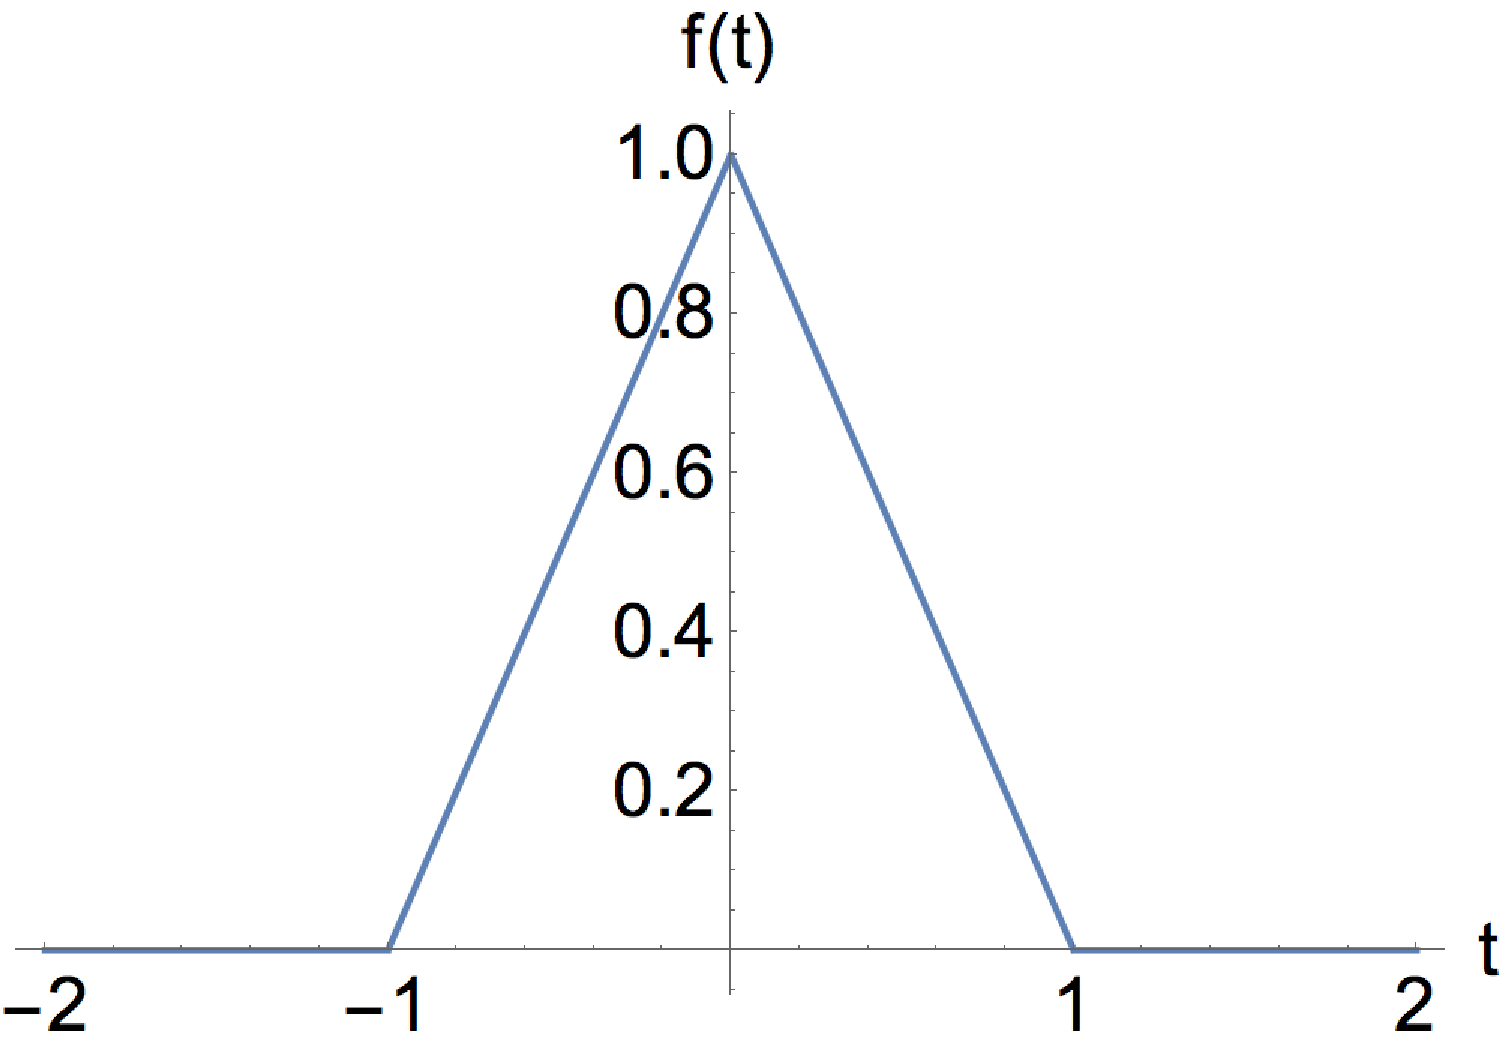
\includegraphics[scale=0.5]{triangle.png} & 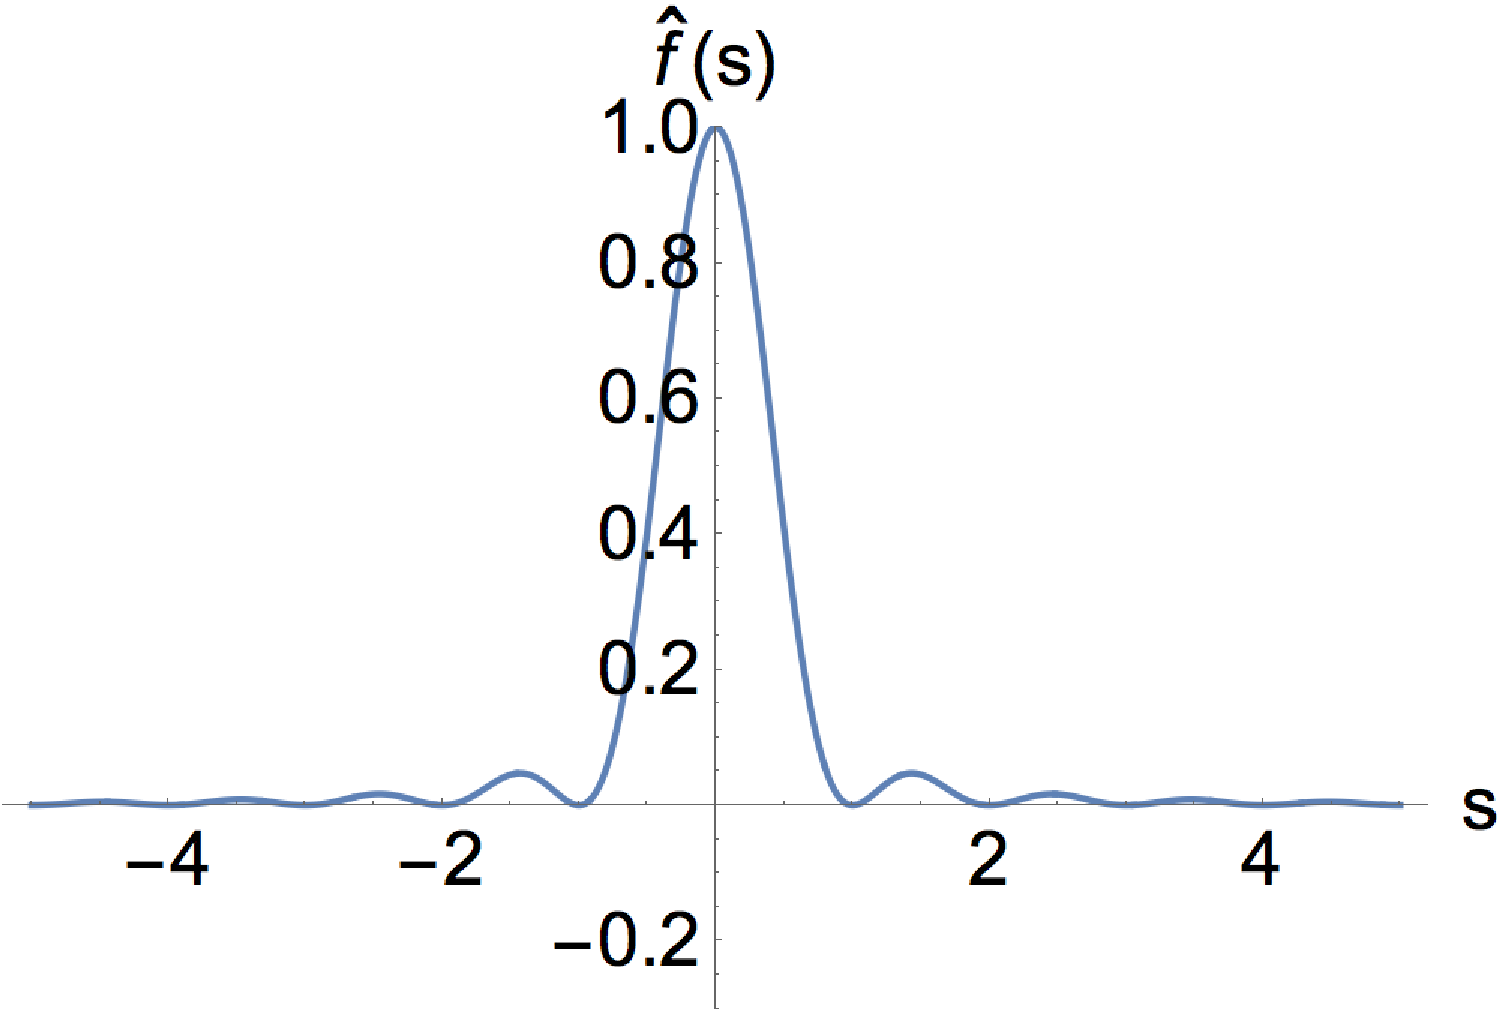
\includegraphics[scale=0.5]{triangleft.png}
\end{tabular}

\subsection*{Solution}
Your answer should be consistent with $F(s=1.5) = 0.045$




%%%%%%%%%%%%%%%%%%%%%%%%%%%%%%%%%
\newpage
%%%%%%%%%%%%%%%%%%%%%%%%%%%%%%%%%
\section{Fourier transform of a Gaussian}

\subsection*{Resources}
\begin{itemize}
    \item Book: Chapter 2.2.2 (\url{https://see.stanford.edu/materials/lsoftaee261/book-fall-07.pdf})
    \item Video: Lecture 7 (\url{https://www.youtube.com/watch?v=mdFETbe1n5Q})
\end{itemize}

\subsection*{Challenge}
Starting from the general formula for Fourier transform, calculate the Fourier transform for the Gaussian function:

\begin{equation}
    f(t) = e^{-\pi t^2}
\end{equation}

The Gaussian function looks like

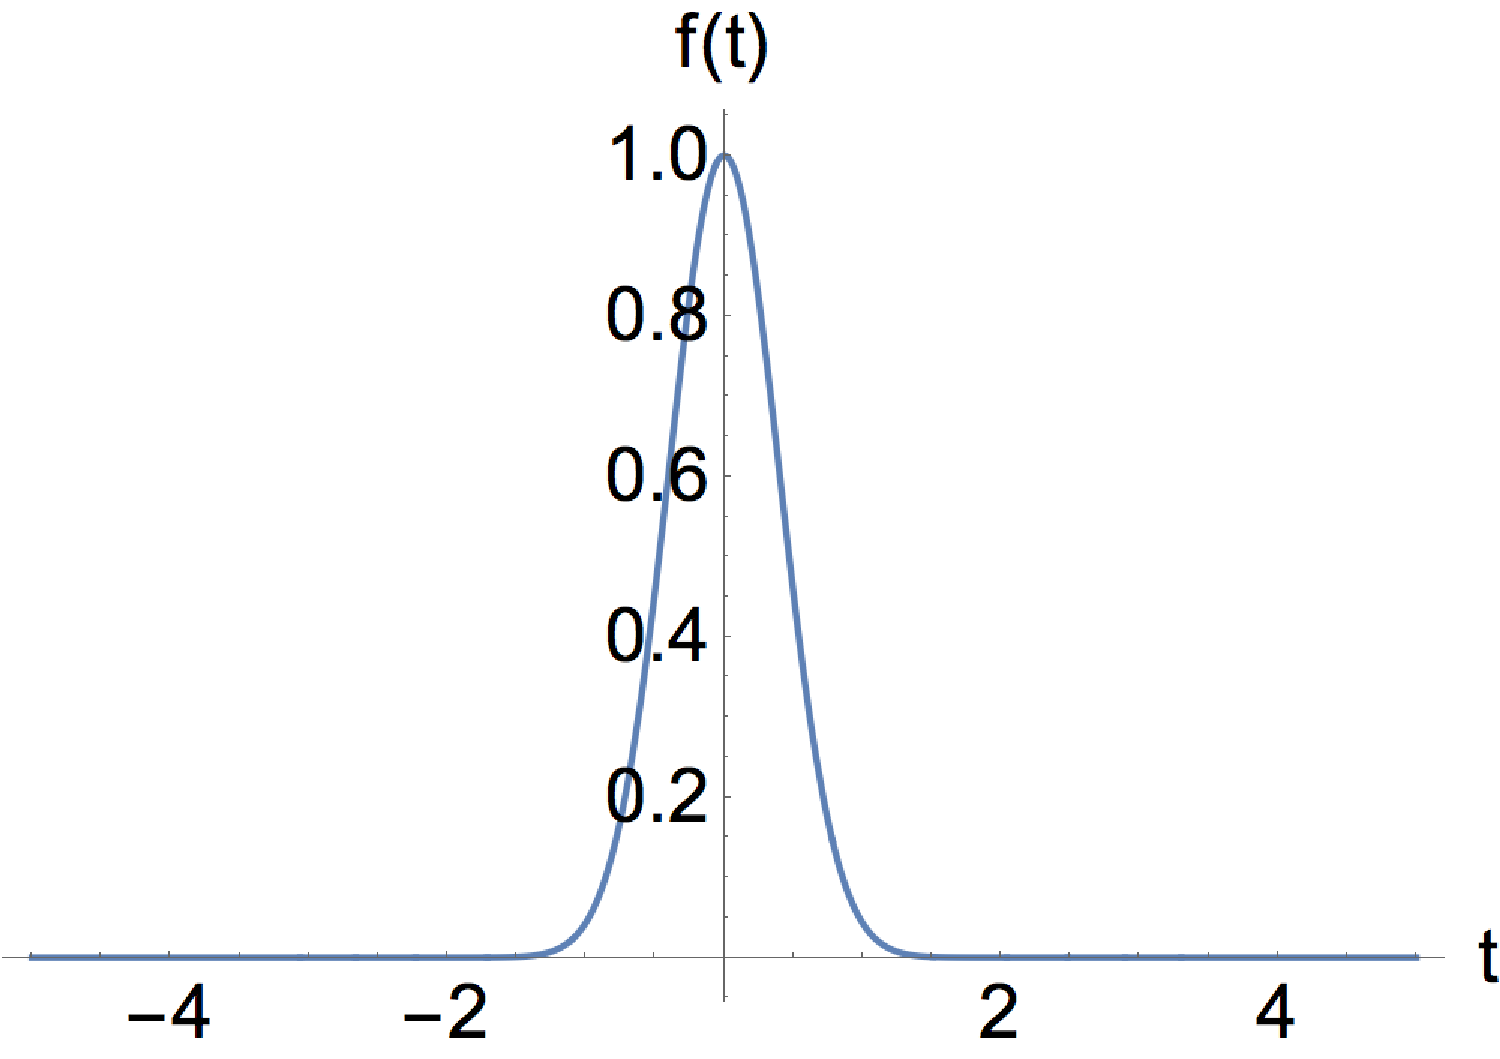
\includegraphics[width=8cm]{gaussian.png}

\subsection*{Solution}
Your answer should be consistent with $F(s=1.5) =$ \num{8.51e-4}




%%%%%%%%%%%%%%%%%%%%%%%%%%%%%%%%%
\newpage
%%%%%%%%%%%%%%%%%%%%%%%%%%%%%%%%%
\section{Fourier transform of a rocket function}

\subsection*{Resources}
\begin{itemize}
    \item Book: Chapter 2.2.6 (\url{https://see.stanford.edu/materials/lsoftaee261/book-fall-07.pdf})
\end{itemize}

\subsection*{Challenge}
Calculate the Fourier Transform for the rocket function:
\begin{equation}
    f(at)=
    \begin{cases}
        2 - |t| & \text{for } 0 \le |t| < \frac{1}{2}\\
        1 - |t| & \text{for } \frac{1}{2} \le |t| \le 1\\
        0 & \text{otherwise}
    \end{cases}
\end{equation}
    
shown below. In graph-form the function and its transform appear as follows:

\begin{tabular}{cc}
    \textbf{Function} & \textbf{Fourier transform} \\
    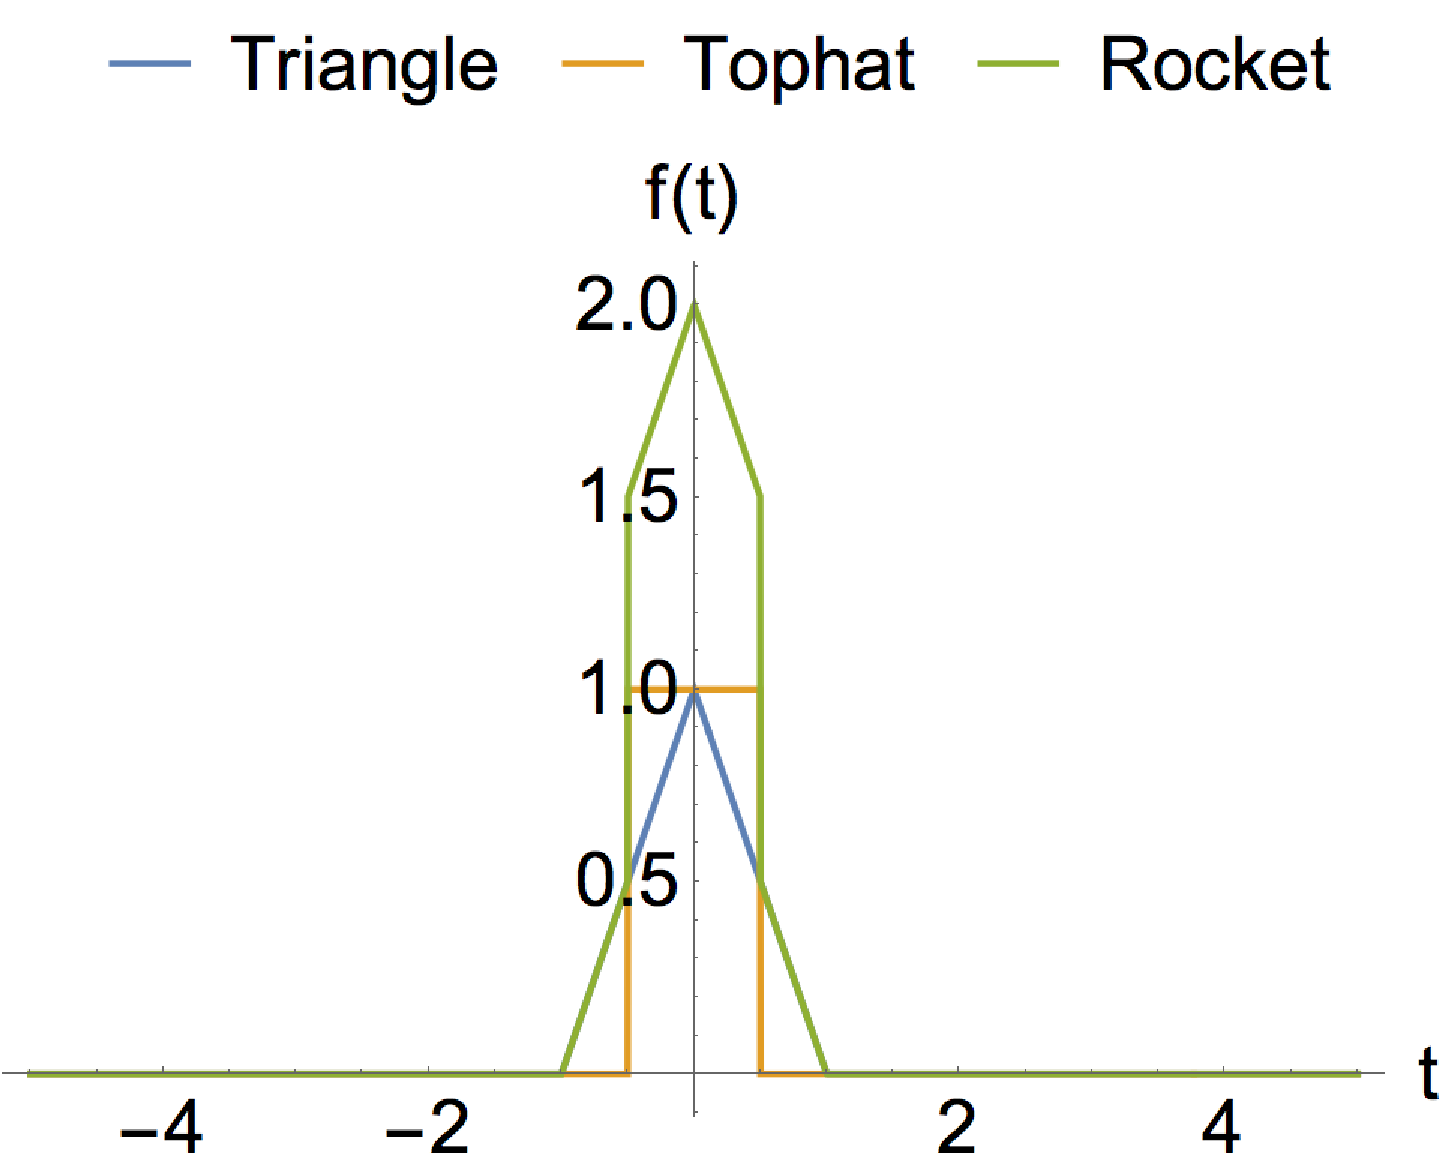
\includegraphics[scale=0.6]{rocket.png} & 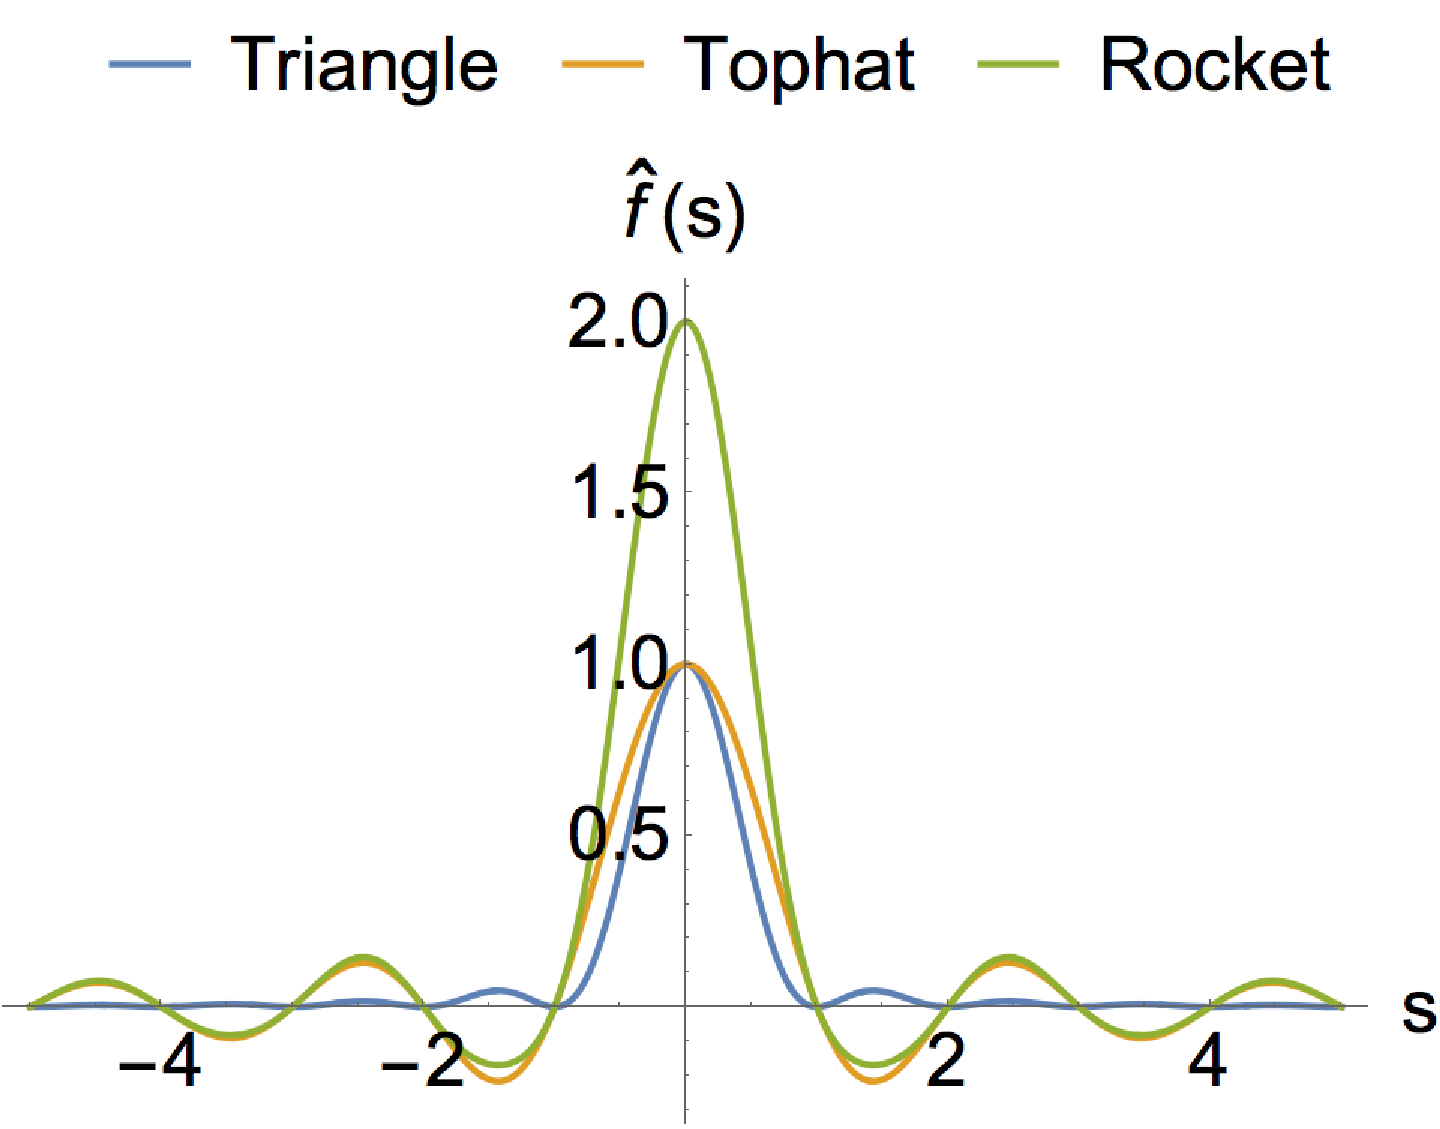
\includegraphics[scale=0.6]{rocketft.png}
\end{tabular}

\subsection*{Solution}
Your answer should be consistent with $F(s=1.5) = -0.17$




\iffalse
%%%%%%%%%%%%%%%%%%%%%%%%%%%%%%%%%
\newpage
%%%%%%%%%%%%%%%%%%%%%%%%%%%%%%%%%
\section{Fourier transform of a shifted window function}

\subsection*{Resources}
\begin{itemize}
    \item Book: Chapter 2.2.7 (\url{https://see.stanford.edu/materials/lsoftaee261/book-fall-07.pdf})
    \item Video lecture 8 from 1:56 to 11:20 (\url{https://youtu.be/wUT1huREHJM?t=1m56s})
\end{itemize}

\subsection*{Challenge}
1. What is meant by a ``phase-shift'' of a signal in time? What does it mean in terms of the window-function here?

2. Calculate the Fourier Transform for the window function delayed by \SI{1}{\second}.

A graph with increasing delay is shown in the figure below. What is happening to the real and imaginary parts of the signal as the delay increases? You considered the original window function in challenge \ref{sec:tophat}.

\begin{tabular}{c}
    \textbf{Function} \\
    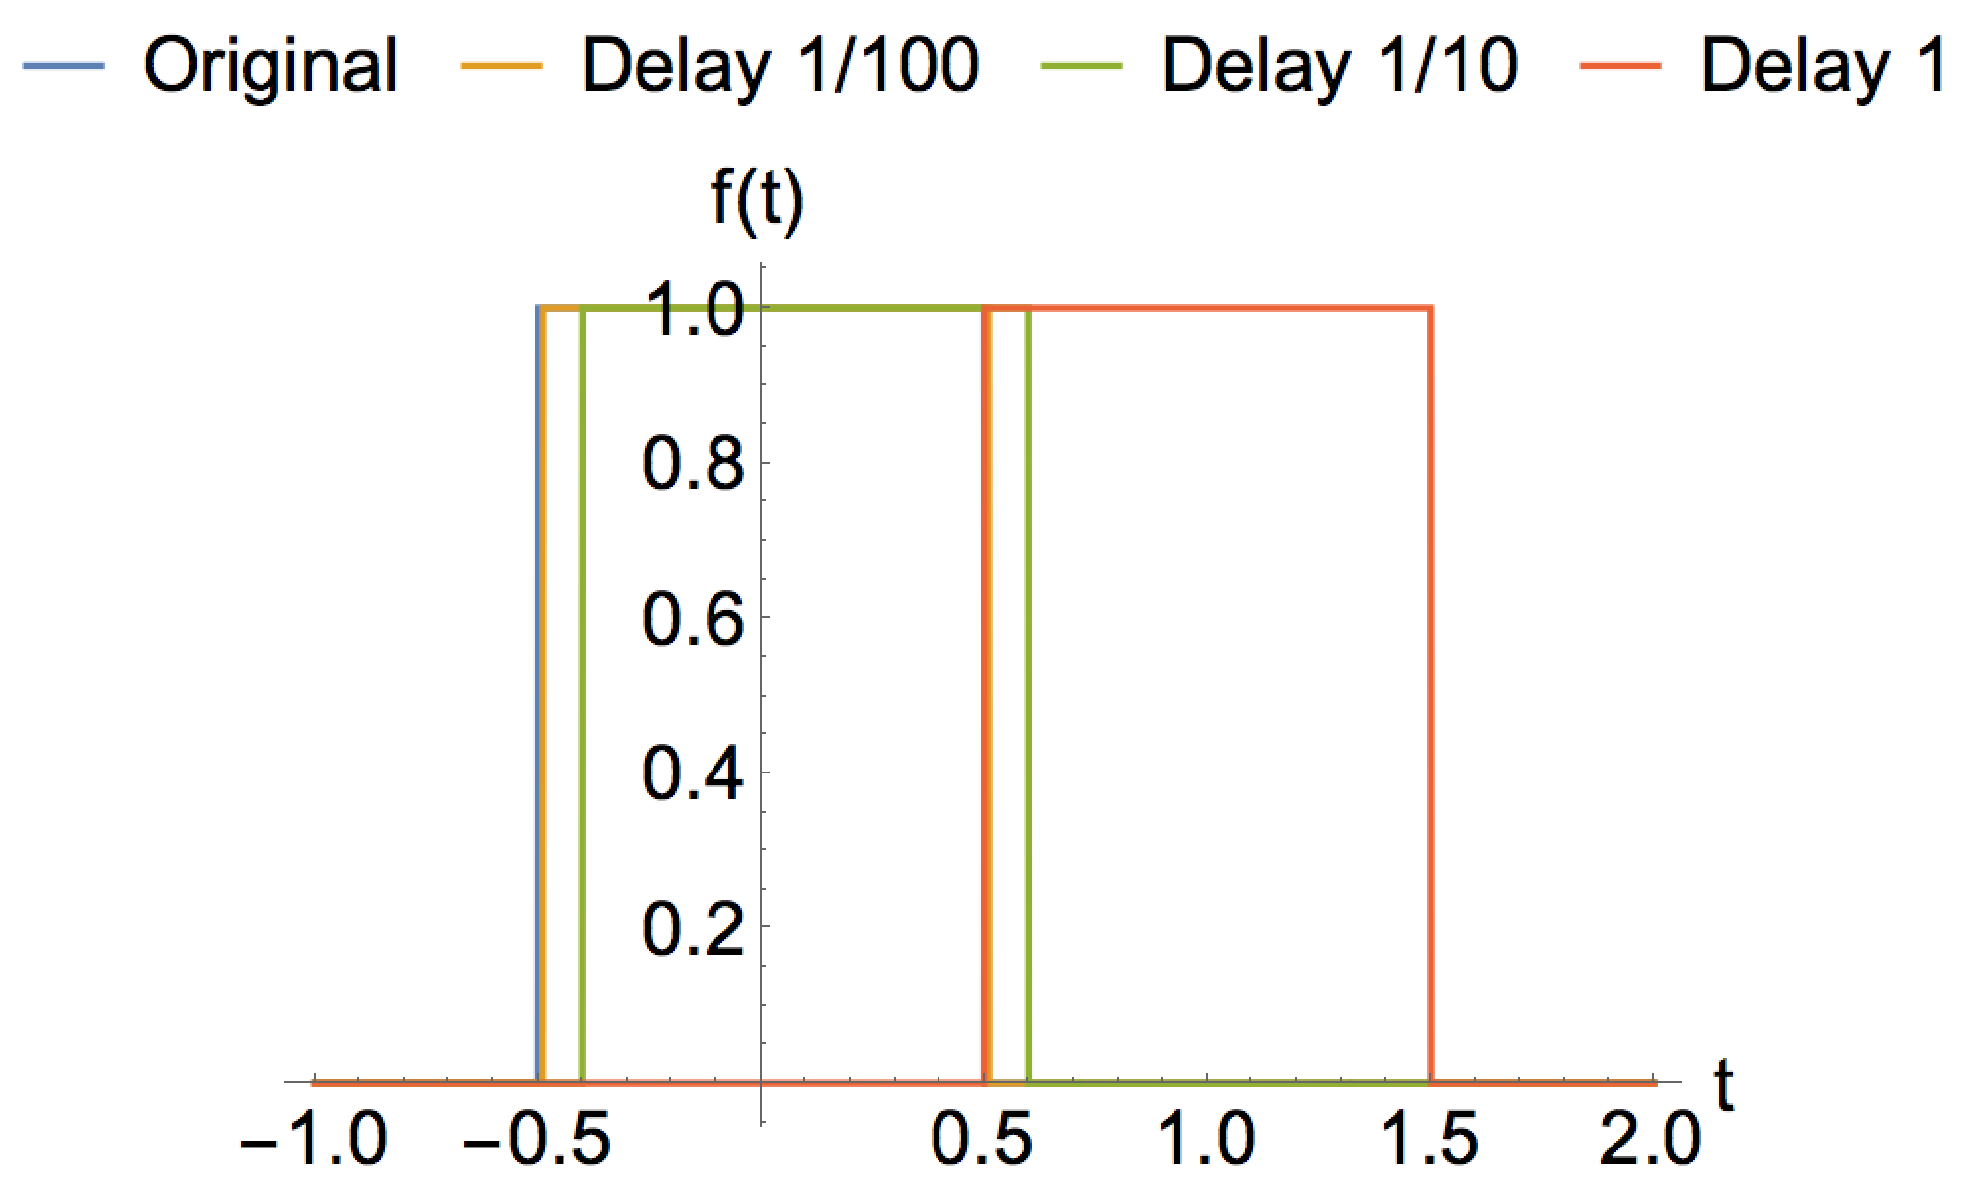
\includegraphics[scale=0.5]{tophatdelay.png}
\end{tabular}

\begin{tabular}{cc}
    \textbf{Fourier transform (real part)} & \textbf{Fourier transform (imaginary part)}\\
    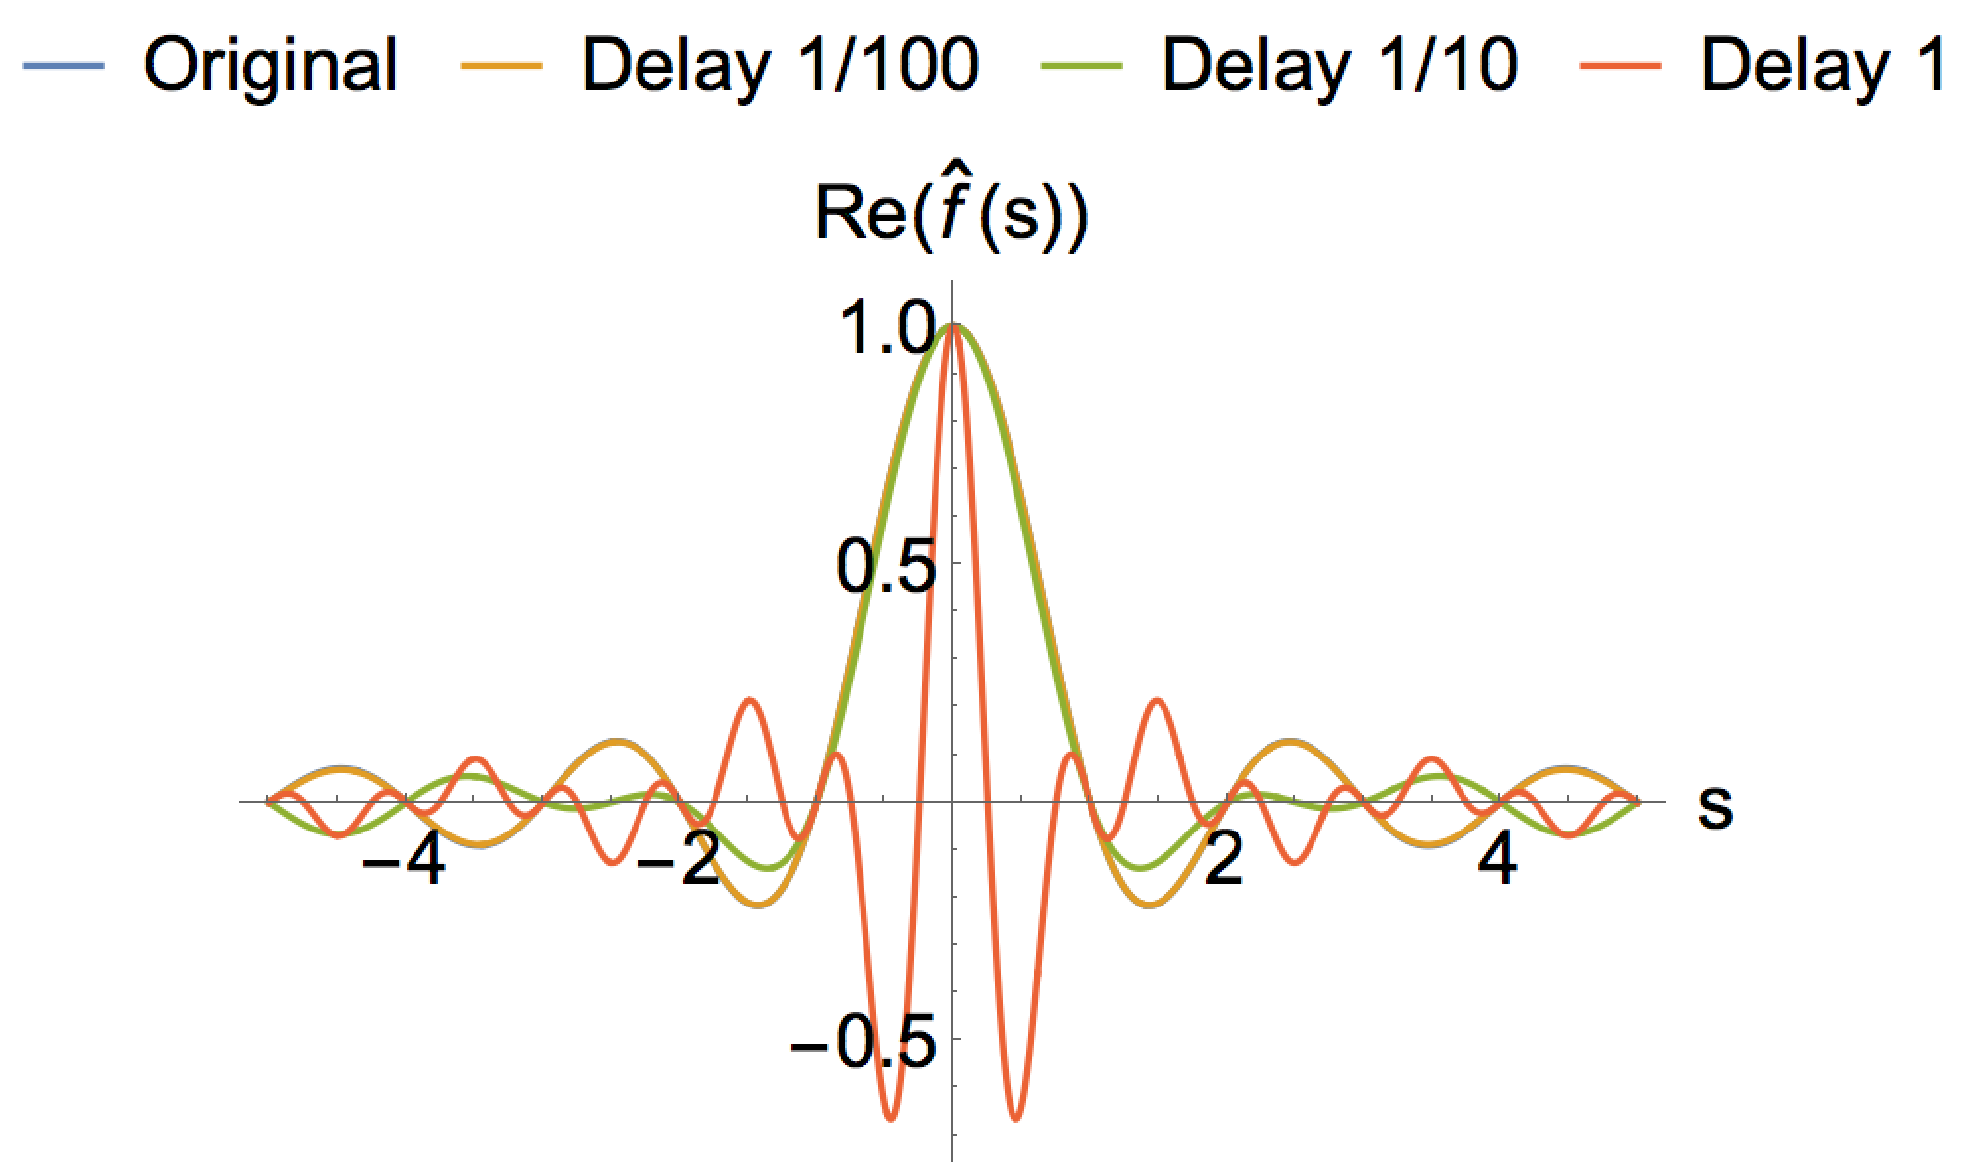
\includegraphics[scale=0.5]{tophatdelayre.png} & 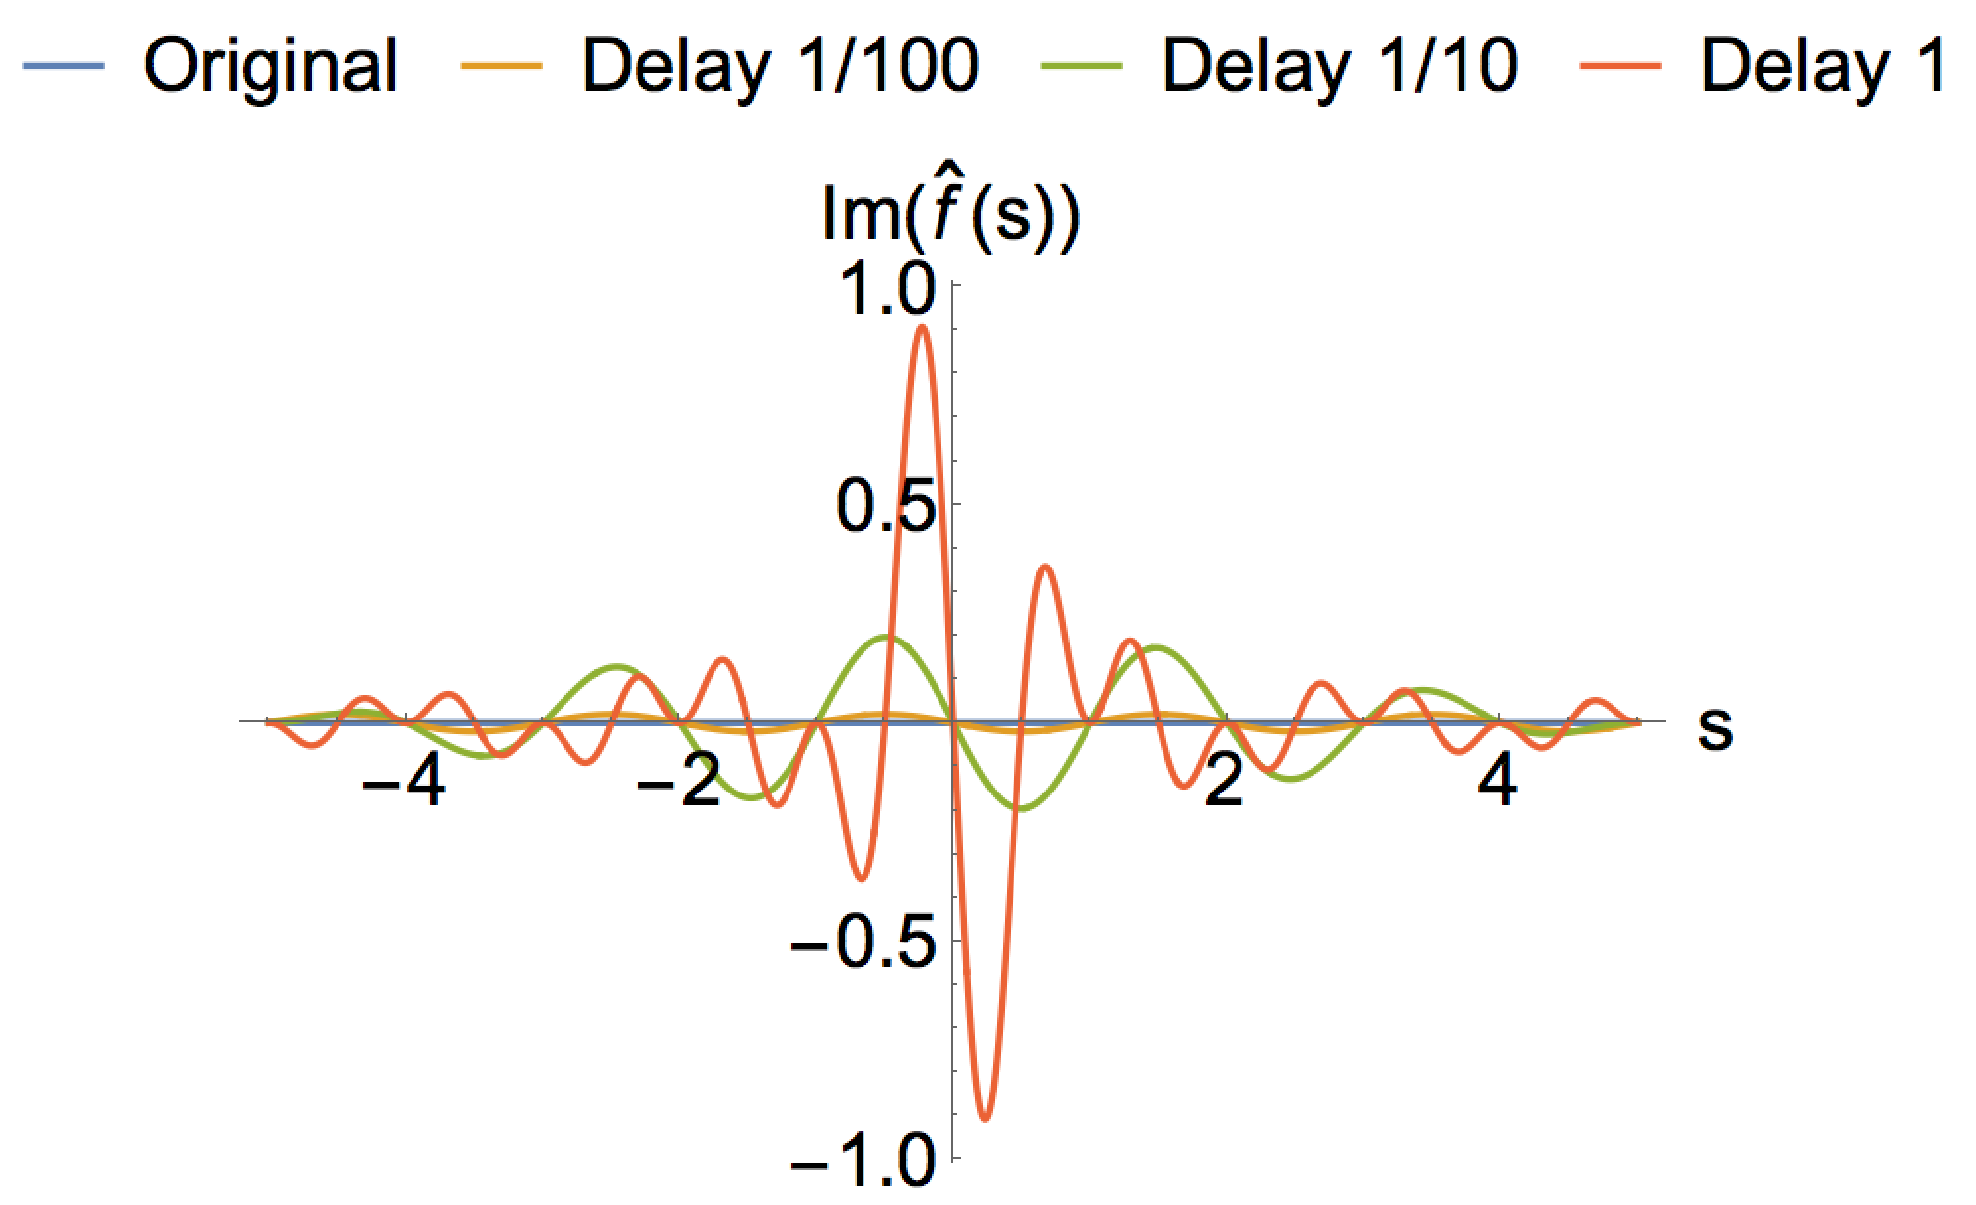
\includegraphics[scale=0.5]{tophatdelayim.png}
\end{tabular}

\subsection*{Solution}
2. You should find that $\hat{f}(s=2.9) = 0.0274405 + 0.0199367i$




%%%%%%%%%%%%%%%%%%%%%%%%%%%%%%%%%
\newpage
%%%%%%%%%%%%%%%%%%%%%%%%%%%%%%%%%
\section{Fourier transform of a stretched triangle function}

\subsection*{Resources}
\begin{itemize}
    \item Book: Chapter 2.2.8 (\url{https://see.stanford.edu/materials/lsoftaee261/book-fall-07.pdf})
    \item Video lecture 8 from 12:12 to 28:50 (\url{https://youtu.be/wUT1huREHJM?t=12m12s})
\end{itemize}

\subsection*{Challenge}
Since this can be a little confusing, please be sure to fully read the listed resource and make sure you understand the reasoning and derivation.

A triangle function of general width can be defined as

\begin{equation}
    f(at)=
    \begin{cases}
        1 - a|t| & \text{for } a|t| < 1\\
        0 & \text{otherwise}
    \end{cases}
\end{equation}

1. In challenge \ref{sec:ft_triangle} the base-width of the triangle was $2$ (ie, $1-(-1)$) and the half-base-width was $1$ (ie, $1-0$). What is the half-base-width for a triangle when $a=2$ and $a=1/2$?

2. Calculate the Fourier Transform $\hat{f}(s)$ for the case where the width of the triangle-function is doubled.

3. Write a few sentences explaining how stretching and squeezing in the time-domain is related to stretching and squeezing in the frequency domain.

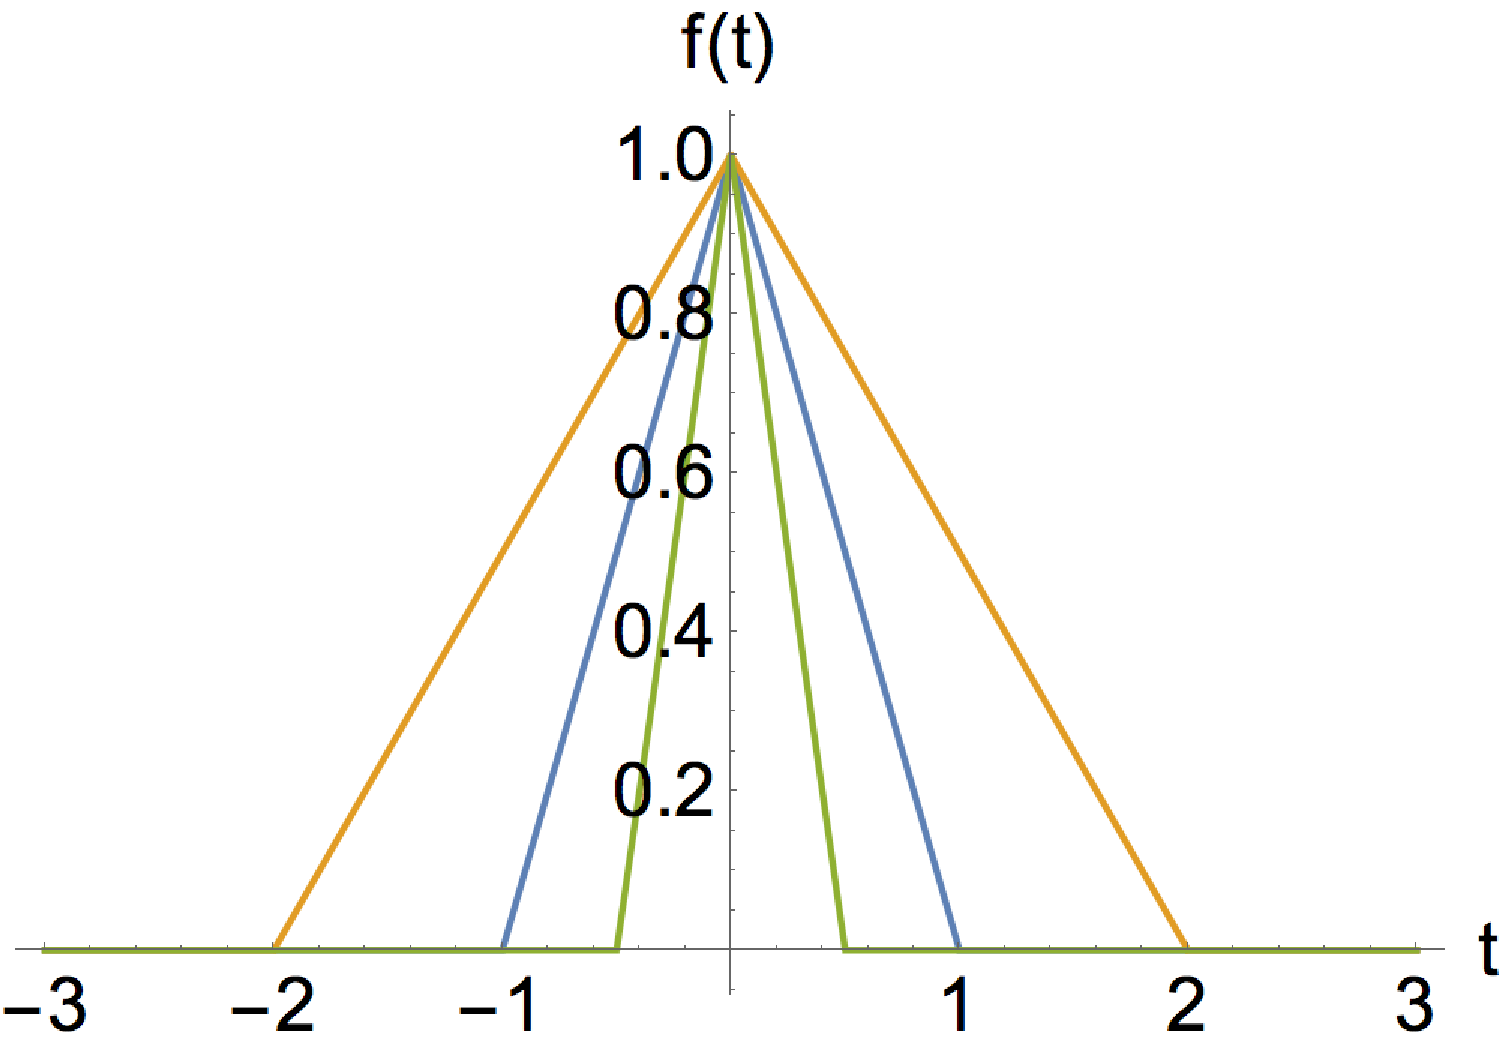
\includegraphics[scale=0.75]{triangledouble.png}

\subsection*{Solution}
1.\\
$a=2$\\
\soltwodp{g}{3cd169}

$a=1/2$\\
\soltwodp{h}{3bb5c8}

2.\\
To check your answer, evaluate the transform at $s=0.1$.\\
$\hat{f}(0.1)=1.75$




%%%%%%%%%%%%%%%%%%%%%%%%%%%%%%%%%
\newpage
%%%%%%%%%%%%%%%%%%%%%%%%%%%%%%%%%
\section{Fourier transform of a shifted-stretched function}
\label{sec:shiftstretch}

\subsection*{Resources}
\begin{itemize}
    \item Book: Chapter 2.2.9 (\url{https://see.stanford.edu/materials/lsoftaee261/book-fall-07.pdf})
\end{itemize}

\subsection*{Challenge}
Calculate the Fourier transform of the signal shown below.

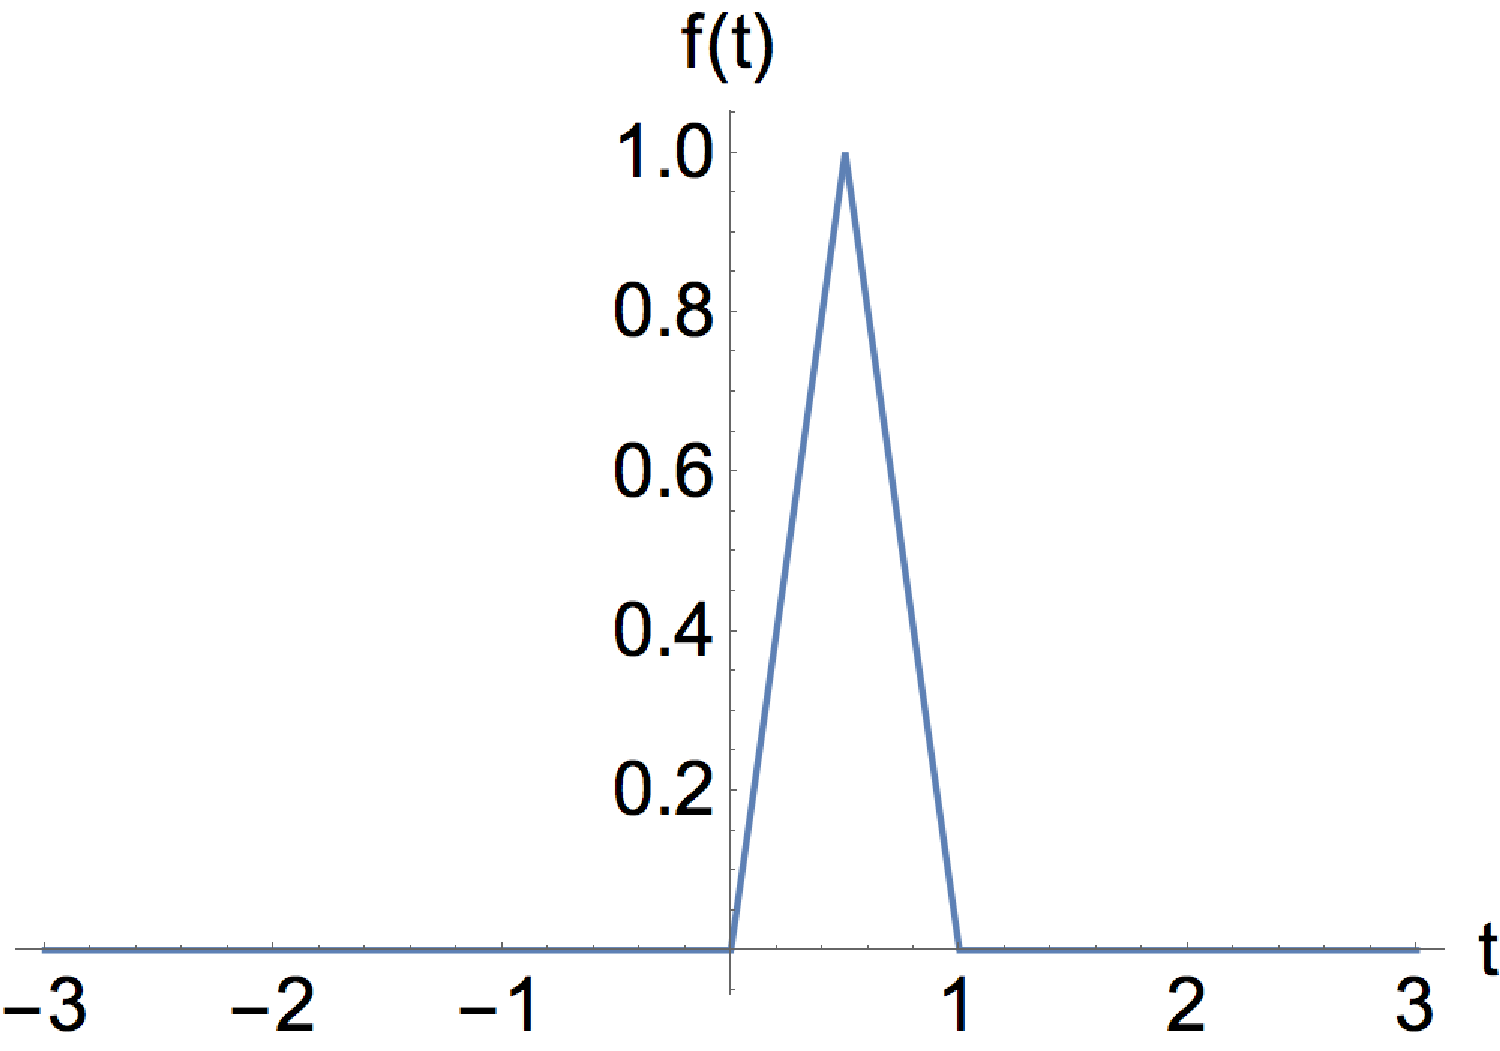
\includegraphics[width=8cm]{triangleshiftsqueeze.png}

\subsection*{Solution}
Your answer should be consistent with $\hat{f}(s=1.1) = -0.155 + 0.050 i$.




%%%%%%%%%%%%%%%%%%%%%%%%%%%%%%%%%
\newpage
%%%%%%%%%%%%%%%%%%%%%%%%%%%%%%%%%
\section{Convolution introduction}

\subsection*{Resources}
\begin{itemize}
    \item Video lecture 8 starting at 32:15: \url{https://youtu.be/wUT1huREHJM?t=32m15s}
\end{itemize}

\subsection*{Comment}
Here we expand our study to convolution; a powerful function for processing signals. Convolution is not immediately intuetive, but Prof. Osgood provides an excellent introduction.

\subsection*{Challenge}
Make notes following the above video deriving the formula relating convolution in the frequency and time domains.




%%%%%%%%%%%%%%%%%%%%%%%%%%%%%%%%%
\newpage
%%%%%%%%%%%%%%%%%%%%%%%%%%%%%%%%%
\section{Filtering}

\subsection*{Resources}
\begin{itemize}
    \item Video lecture 9 until 24:15: \url{https://www.youtube.com/watch?v=NrOR2qMVWOs}
\end{itemize}

\subsection*{Comment}
The above video includes an excellent example of using fourier analysis in a scientific context, including its application in filters.

The challenge below asks you to watch to 24:15, however after this point he goes on to describe the futility of trying to visualise convolution in the time-domain. Nevertheless, the graphics on convolution on Wikipedia [1] (especially these: [2a,b]) I think go some way to visualising what's happening in the time-domain.

1: \url{https://en.wikipedia.org/wiki/Convolution}\\
2a: \url{https://en.wikipedia.org/wiki/Convolution\#/media/File:Convolution_of_box_signal_with_itself2.gif}\\
2b: \url{https://en.wikipedia.org/wiki/Convolution\#/media/File:Convolution_of_spiky_function_with_box2.gif}

For your reference, turbidity standards of 5, 50, and 500 Nephelometric Turbidity Units (left to right respectively) are shown here:\\
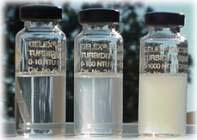
\includegraphics{turbidity.png}\\
\emph{Source: \url{https://en.wikipedia.org/wiki/Turbidity}}

\subsection*{Challenge}
1. Take notes following the above video until 24:15. There is a lot of useful information here. The questions below highlight the key points that I want you to understand, however they do not cover everything, so please be sure to follow the video.

2. Using a few sentences and diagrams, describe an ideal low-pass, high-pass and band-pass filter. How can they be applied in the frequency domain to influence the signal in the time-domain?

3. Write a few sentences and equations describing how convolution in the time-domain is related to signal multiplication in the frequency-domain.


%%%%%%%%%%%%%%%%%%%%%%%%%%%%%%%%%
\newpage
%%%%%%%%%%%%%%%%%%%%%%%%%%%%%%%%%
\section{Convolution with a window function}

\subsection*{Comment}
The ``signal'' here is $g(t-\tau)$ and the ``window function'' is $f(\tau)$.

\subsection*{Challenge}
1. Consider that you have a (somewhat unrealistic but mathematically manageable) input signal that varies as $g(t-\tau)=(t-\tau)^2$ with time. 

Obtain the convolution of the signal $(f \star g)(t)$ with a window function:
\begin{equation}
    f(\tau)=
    \begin{cases}
        1 & \text{for } -1/2 < \tau < 1/2\\
        0 & \text{otherwise}
    \end{cases}
\end{equation}

2. Compare the answer above when $t=0$ with direct integration of $\tau^2$ between $-1/2$ and $1/2$. Why are they the same?

\subsection*{Solution}
\hash{ppp}{290253}




%%%%%%%%%%%%%%%%%%%%%%%%%%%%%%%%%%
%\newpage
%%%%%%%%%%%%%%%%%%%%%%%%%%%%%%%%%%
%\section{Convolution with a continuous function}
%
%\subsection*{Challenge}
%Consider that you have a (somewhat unrealistic but mathematically manageable) input signal that varies with time $\tau$ as $f(\tau)=\tau$.  Apply a filter to the signal that is defined at time $t$ as $e^{-|t|}$.
%
%\emph{Hint: $\int_{-\infty}^{\infty} \text{(even function)} = 2 \int_{0}^{\infty} \text{(even function)}$.}
%
%To check your answer, substitute $t=1$ into your final answer.
%
%\subsection*{Solution}
%\hash{qqq}{e48f28}




%%%%%%%%%%%%%%%%%%%%%%%%%%%%%%%%%%
%\newpage
%%%%%%%%%%%%%%%%%%%%%%%%%%%%%%%%%%
%\section{Inequalities}
%
%\subsection*{Challenge}
%1. Re-write $-1/2 < t - \tau$ in the form $f(\tau) < t$ replacing $f(\tau)$ with appropriate expressions.
%
%2. Re-write $t - \tau < 1/2$ in the form $t < f(\tau)$ replacing $f(\tau)$ with appropriate expressions.
%
%3. Re-write $-1/2 < t - \tau < 1/2$ in the form $f(\tau) < t < g(\tau)$ replacing $f(\tau)$ and $g(\tau)$ with appropriate expressions.
%
%\subsection*{Solution}
%To check your solutions, substitute $\tau=1/2$ into the final expressions:
%
%1. $f(1/2)$: \hash{kkk}{115edb}\\
%2. $f(1/2)$: \hash{mmm}{6d64cd}\\
%3. $f(1/2)$: \hash{nnn}{414d80} and $g(1/2)$: \hash{ooo}{3ec4d7}




%%%%%%%%%%%%%%%%%%%%%%%%%%%%%%%%%%
%\newpage
%%%%%%%%%%%%%%%%%%%%%%%%%%%%%%%%%%
%\section{Touching window functions}
%\label{sec:touchingwindows}
%
%\subsection*{Challenge}
%1. Consider two window functions $f$ and $g$.
%\begin{equation}
%    f(\tau)=
%    \begin{cases}
%        1 & \text{for } -1/2 < \tau < 1/2\\
%        0 & \text{otherwise}
%    \end{cases}
%\end{equation}
%\begin{equation}
%    g(t-\tau)=
%    \begin{cases}
%        1 & \text{for } -1/2 < t-\tau < 1/2\\
%        0 & \text{otherwise}
%    \end{cases}
%\end{equation}
%You can imagine a fixed window function $f$ and a shiftable window-function $g$ (depending on the value of $t$). What is the value of $t$ in the following situations?
%
%a) The left side of window $f$ and the right side of window $g$ are touching.\\
%b) Complete overlap of windows $f$ and $g$.\\
%c) The right side of window $f$ and the left side of window $g$ are touching.
%
%2.\\
%a) Write a function that describes the position of the left-hand-side of window function $g$ at time $t$.\\
%b) Write a function that describes the position of the right-hand-side of window function $g$ at time $t$.\\
%To check your answers, substitute $t=1$ into your expressions.
%
%\subsection*{Solution}
%1.a) \hash{rrr}{1e3803}\\
%1.b) \hash{sss}{171271}\\
%1.c) \hash{ttt}{95acc3}\\
%
%2.a) \hash{uuu}{e27eca}\\
%2.b) \hash{vvv}{23da5b}




%%%%%%%%%%%%%%%%%%%%%%%%%%%%%%%%%
\newpage
%%%%%%%%%%%%%%%%%%%%%%%%%%%%%%%%%
\section{Convolution of two window functions}

\subsection*{Challenge}
%1. Show that the convolution of the two window functions in challenge \ref{sec:touchingwindows} in the time-domain results in the triangle function
%\begin{equation}
%    h(t)=
%    \begin{cases}
%        1+t & \text{for } 1 < t < 0\\
%        1-t & \text{for } 0 < t < 1\\
%        0 & \text{otherwise}
%    \end{cases}
%\end{equation}

In challenge \ref{sec:tophat} you calculated the spectrum of a window function. Imagine here you have two window functions $f(t)$ and $g(\tau)$.

\begin{equation}
    f(t)=
    \begin{cases}
        1 & \text{for } |t| < 1/2 \\
        0 & \text{for } |t| > 1/2
    \end{cases}
\end{equation}

\begin{equation}
    g(\tau)=
    \begin{cases}
        1 & \text{for } |\tau| < 1/2 \\
        0 & \text{for } |\tau| > 1/2
    \end{cases}
\end{equation}

1. Use your knowledge of the window-function in the frequency domain from challenge \ref{sec:tophat} to calculate the frequency-domain spectrum of the convolution of the two window functions.

2. Compare your answer to that obtained in challenge \ref{sec:ft_triangle}. What is the resulting function in the time-domain? \emph{This should be possible by comparison, without calculation.}

\subsection*{Solution}
To check your answer, substitute $s=1$ into your answers

1. 0.71

2. \hash{www}{9a90c0}


\fi
% Discrete (L19-10:30,L20)



% Calculate fourier transform of dirichlet window https://www.youtube.com/watch?annotation_id=annotation_655167&feature=iv&src_vid=8JKb9UN6W4c&v=_HJH3MekMHY

%\chapter{Discrete Fourier Transform}
%\section{Introduction to digital signals}

\subsection*{Resources}

The following pages are based on slides developed by Prof. Maraso Yamashiro for the 2015 class on Fourier Analysis. Please work through the slides on the following pages and view the video afterwards.

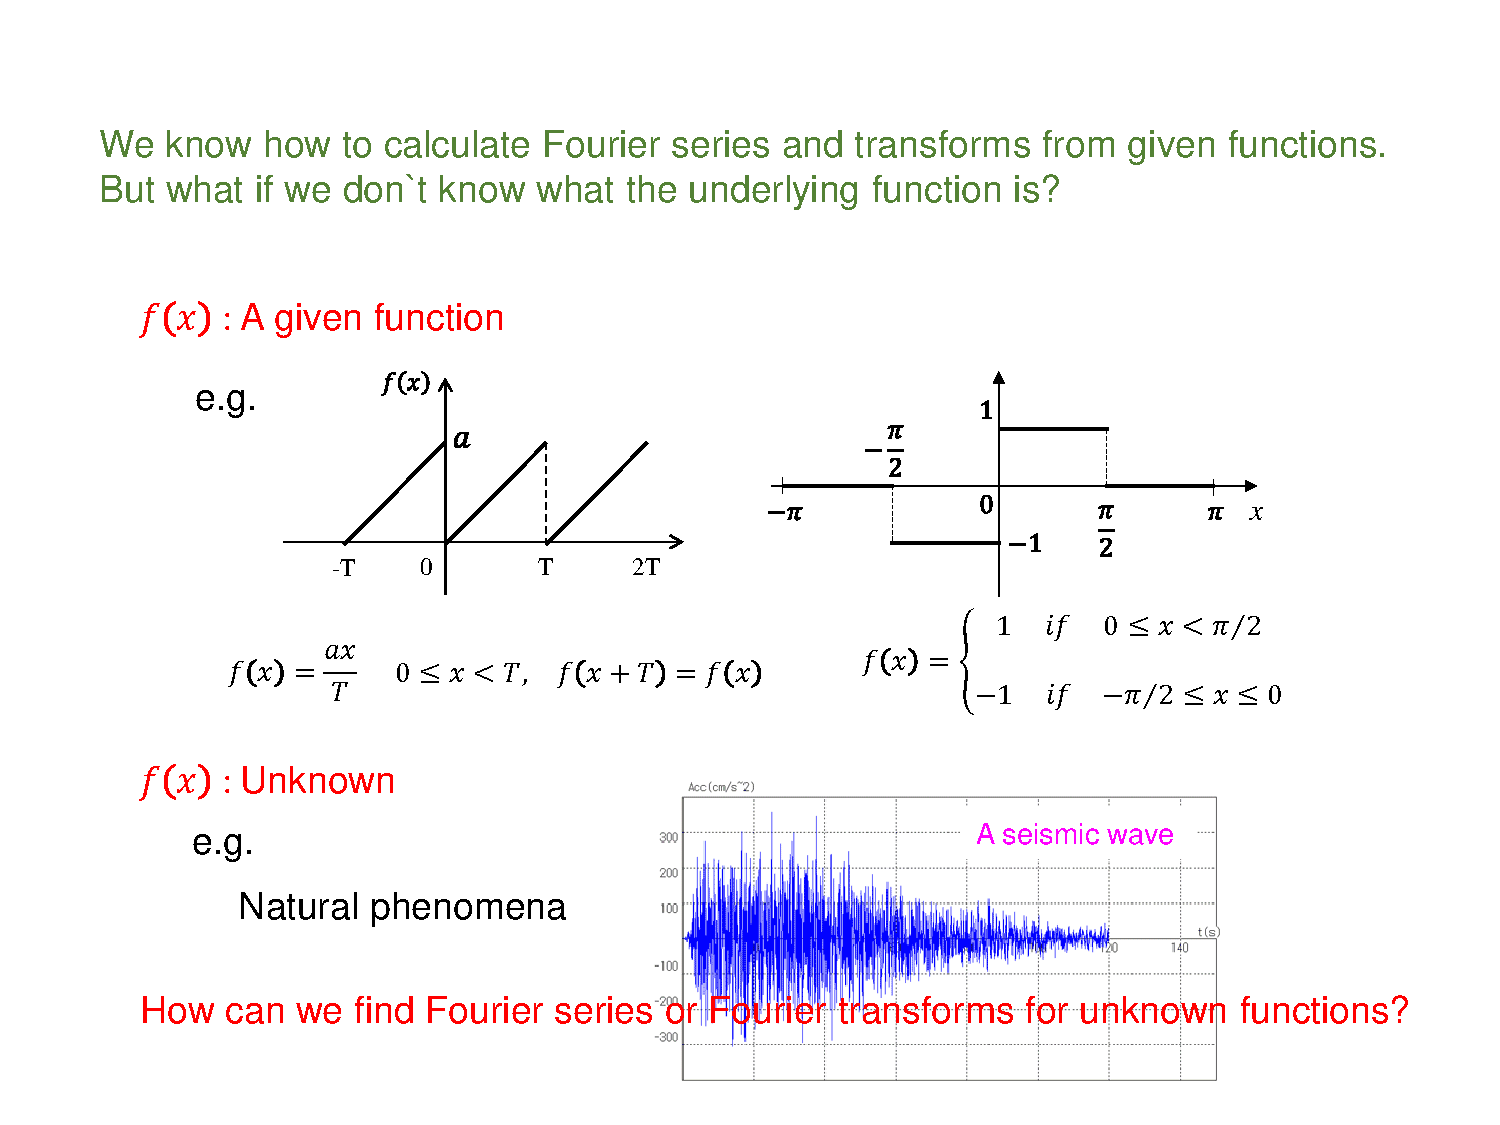
\includepdf[pages=-,pagecommand={},width=\textwidth,nup=1x2,frame=true]{discrete_1-5.pdf}

\begin{itemize}
    \item Video: \url{https://www.youtube.com/watch?v=yWqrx08UeUs&feature=youtu.be&t=47s}
\end{itemize}

\subsection*{Challenge}
1. An audio CD can record frequencies up to 44.1 kHz. Consider how often you would need to sample a sound in order to reproduce frequencies up to 44.1 kHz. What is the highest sampling frequency that experiences aliasing?

2. Write a sentence or two summarising what aliasing is and the Nyquist sampling theorem.

\subsection*{Solutions}
1.\\
\soltwodp{x}{43ef8f}

2. Check your answer with your partner and discuss any differences. Ask the teacher if you are unsure.

% Add something on quantisation?




%%%%%%%%%%%%%%%%%%%%%%%%%%%%%%%%%
\newpage
%%%%%%%%%%%%%%%%%%%%%%%%%%%%%%%%%
\section{Discrete Fourier Transform: Coefficients}

\subsection*{Resources}

The following pages are based on slides developed by Prof. Maraso Yamashiro for the 2015 class on Fourier Analysis. The slides have been lightly modified for notation differences.
 %Please follow the derivation on the following pages.
Note that the equation for the discrete Fourier Transform on the 5th slide should read

\begin{equation}
    \hat{f}_n = N c_n = \sum_{k=0}^{N-1} f_k e^{-i 2 \pi n x_k}
\end{equation}

and not $e^{-inx_k}$ (my mistake).

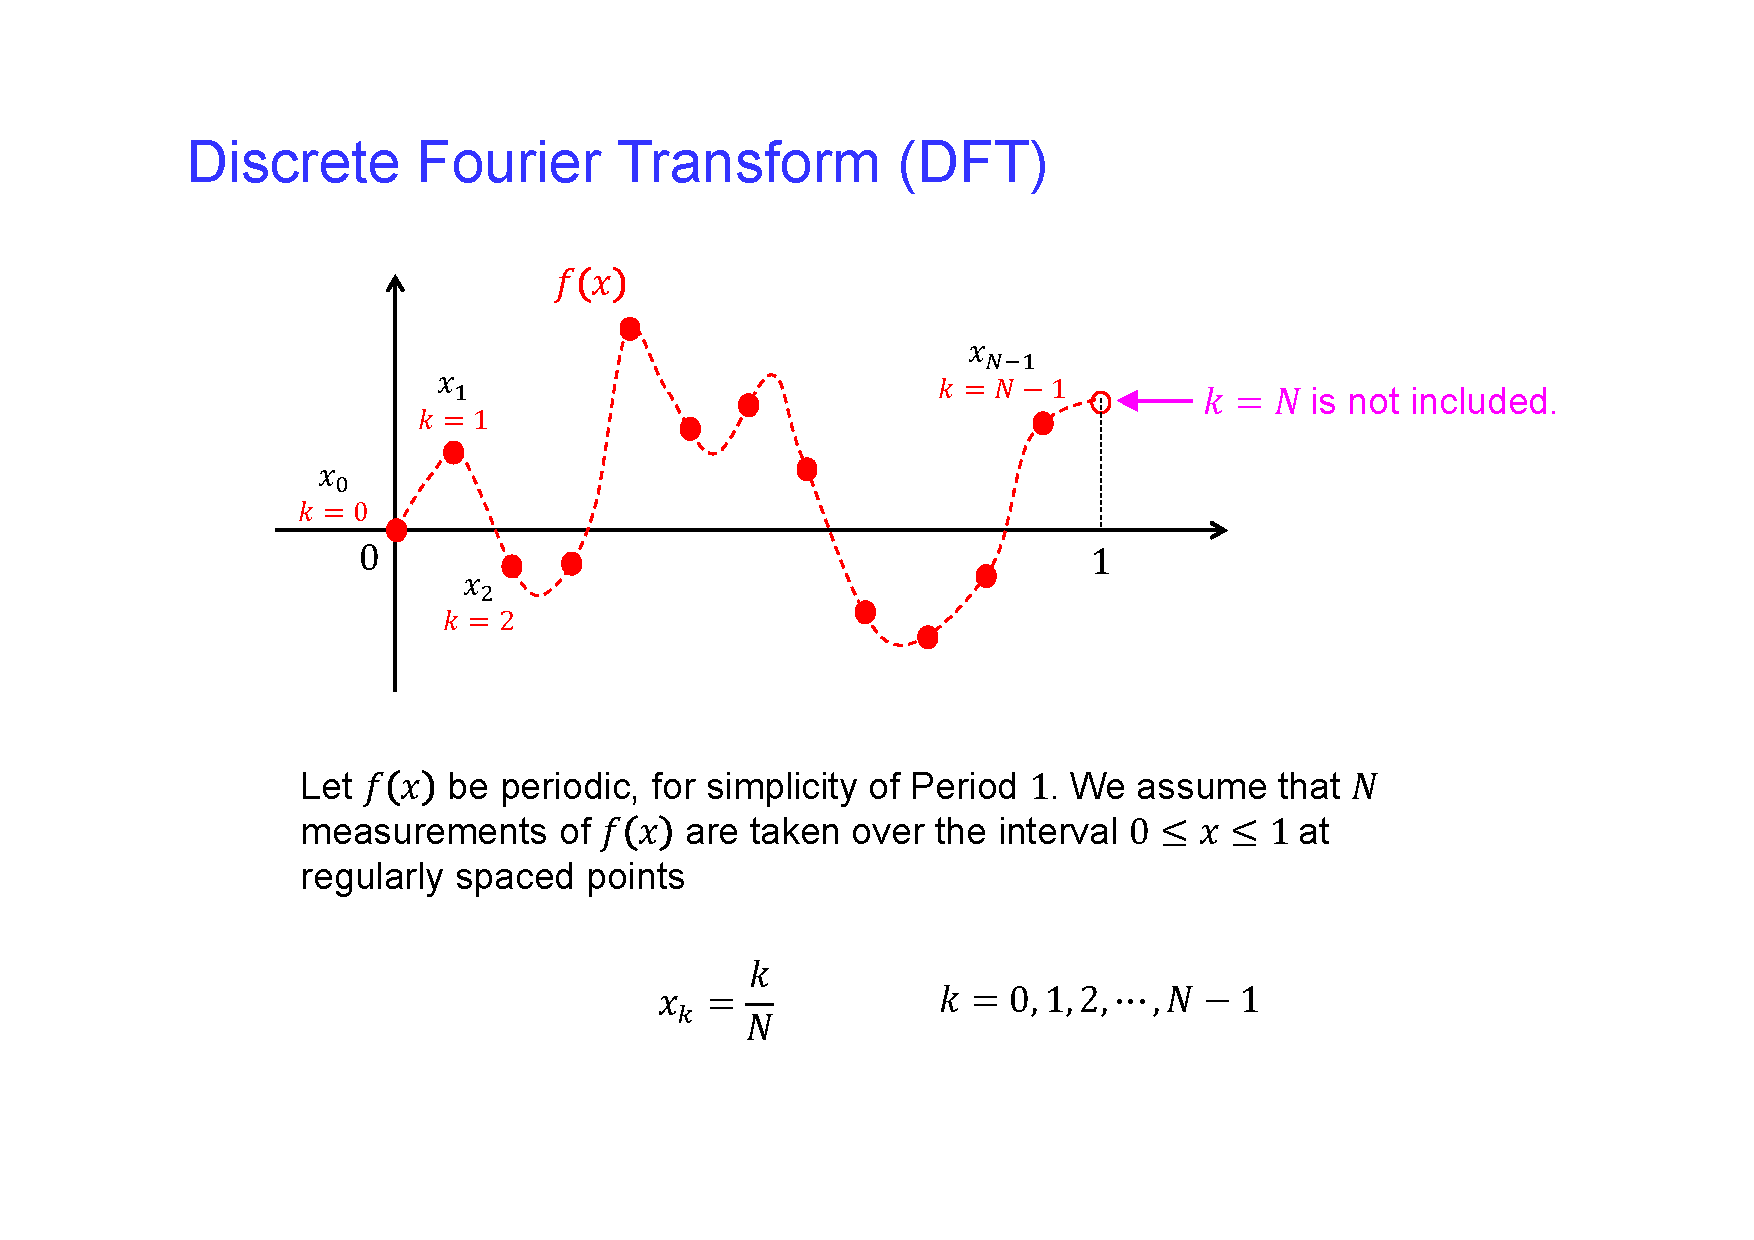
\includepdf[pages=-,pagecommand={},width=\textwidth,nup=1x2,frame=true]{discrete_10-15.pdf}

The challenge below considers sampling of a 1 Hz sine-wave 8 times per second, sampling at time 0, $\frac{1}{8}$, \ldots, $\frac{7}{8}$:

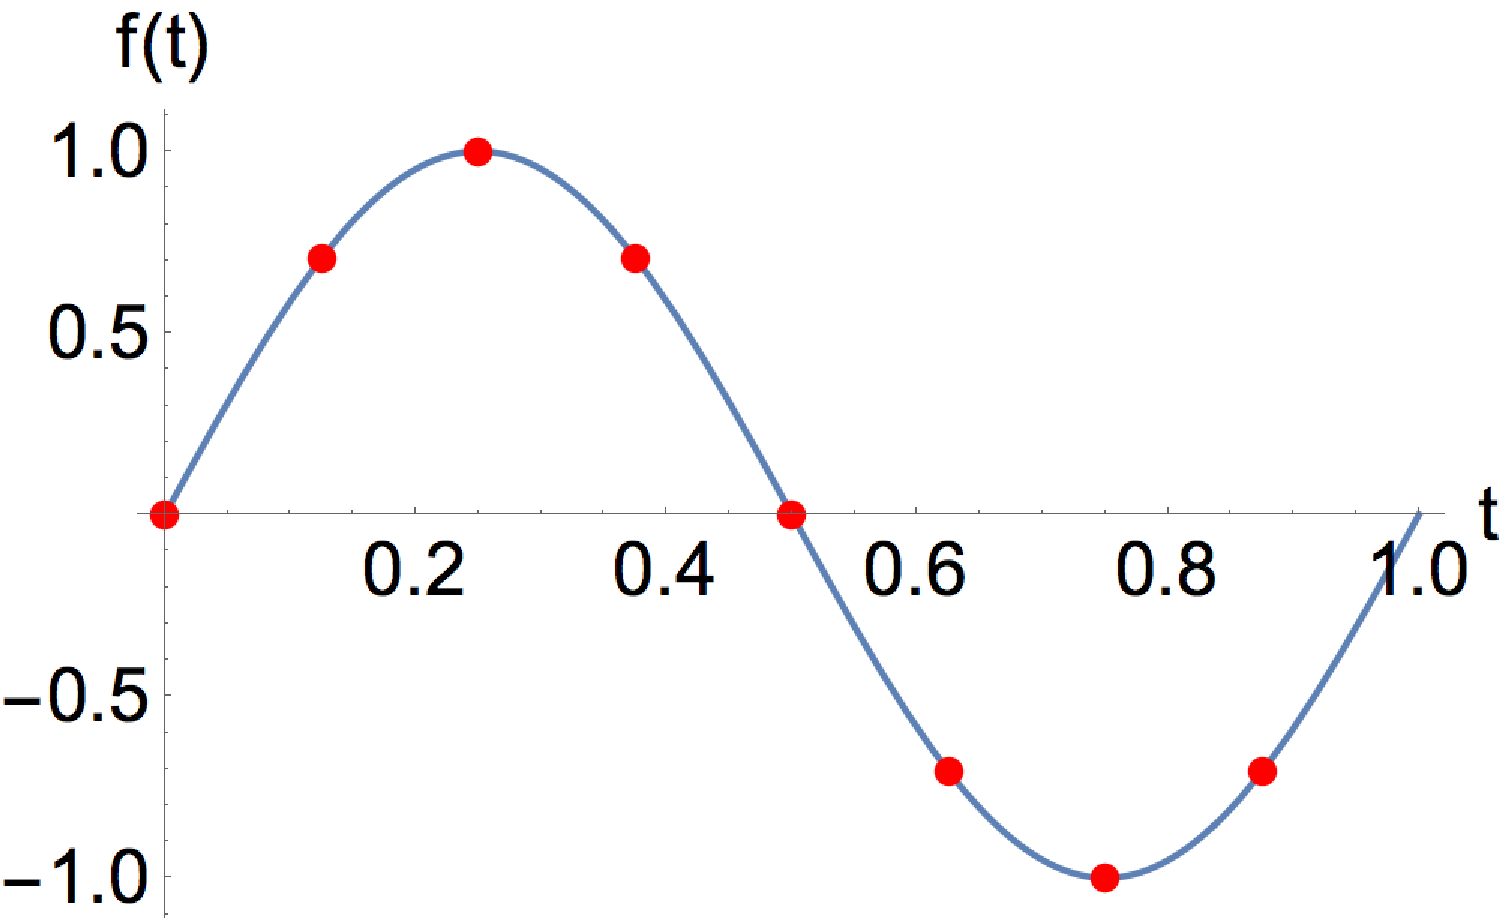
\includegraphics[scale=0.75]{sinedft.png}

This yields sample values of

\begin{equation}
f = \left(
\begin{array}{c}
 0 \\
 1/\sqrt{2} \\
 1 \\
 1/\sqrt{2} \\
 0 \\
 -1/\sqrt{2} \\
 -1 \\
 -1/\sqrt{2} \\
\end{array}
\right)
\end{equation}

\subsection*{Challenge}
Calculate the missing values A-H in the following calculation of the frequency spectrum. To a certain extent you may be able to pattern-match to guess the values, but please be sure that you practise the calculation method too, since that is the main learning objective here.
% NT: Some people do pattern-matching. Maybe need to do a smaller problem where calculation is the only way (can be partial like the previous sensei's 4x4 non-sinusoidal function)


\begin{equation}
    F_8 = 
    \left(
        \begin{array}{cccccccc}
             1 & \textbf{A} & \textbf{B} & 1 & 1 & 1 & 1 & 1 \\
             1 & \textbf{C} & \textbf{D} & -\frac{1+i}{\sqrt{2}} & -1 & -\frac{1-i}{\sqrt{2}} & i & \frac{1+i}{\sqrt{2}} \\
             1 & \textbf{E} & \textbf{F} & i & 1 & -i & -1 & i \\
             1 & -\frac{1+i}{\sqrt{2}} & i & \frac{1-i}{\sqrt{2}} & -1 & \frac{1+i}{\sqrt{2}} & -i & -\frac{1-i}{\sqrt{2}} \\
             1 & -1 & 1 & -1 & 1 & -1 & 1 & -1 \\
             1 & -\frac{1-i}{\sqrt{2}} & -i & \frac{1+i}{\sqrt{2}} & -1 & \frac{1-i}{\sqrt{2}} & i & -\frac{1+i}{\sqrt{2}} \\
             1 & i & -1 & -i & 1 & i & -1 & -i \\
             1 & \frac{1+i}{\sqrt{2}} & i & -\frac{1-i}{\sqrt{2}} & -1 & -\frac{1+i}{\sqrt{2}} & -i & \frac{1-i}{\sqrt{2}} \\
        \end{array}
    \right) 
\end{equation}


\begin{equation}
    \hat{f} =
    \left(
        \begin{array}{c}
             \textbf{G} \\
             \textbf{H} \\
             0 \\
             0 \\
             0 \\
             0 \\
             0 \\
             4 i \\
        \end{array}
    \right)
\end{equation}

\subsection*{Solutions}

Enter imaginary numbers as indicated below. For example: $-1/\sqrt{2}-i/\sqrt{2}$ with a prefix of ``a'' would be entered as ``are(-0.71)im(-0.71)'', $-i$ would be entered as ``are(0.00)im(-1.00)'' and $-1$ would be ``are(-1.00)im(0.00)''.

\textbf{A}\\
\solimagtwodp{a}{95c9e4}

\textbf{B}\\
\solimagtwodp{b}{ec0ffd}

\textbf{C}\\
\solimagtwodp{c}{13085b}

\textbf{D}\\
\solimagtwodp{d}{d01771}

\textbf{E}\\
\solimagtwodp{e}{332be1}

\textbf{F}\\
\solimagtwodp{f}{27b237}

\textbf{G}\\
\solimagtwodp{g}{cbd79b}

\textbf{H}\\
\solimagtwodp{h}{293fff}




%%%%%%%%%%%%%%%%%%%%%%%%%%%%%%%%%
\newpage
%%%%%%%%%%%%%%%%%%%%%%%%%%%%%%%%%
\section{Discrete Fourier Transform: Analysis}

\subsection*{Resources}
Having identified the frequency spectrum, it is possible then to analyse the frequencies of the signal. The video listed below provides a nice introduction into understanding our frequency spectrum. Note that it uses the ``j'' representation of imaginary numbers (instead of ``i'').

\begin{itemize}
    \item Video: \url{https://www.youtube.com/watch?v=mkGsMWi_j4Q}
\end{itemize}

\subsection*{Comment}
The video discusses the phase of the signal as the angle formed by rotating anti-clockwise from an arrow pointing in the positive direction along the real axis. You saw in challenge \ref{sec:ftofsinandcos} how the continuous Fourier transform of a cosine function yields real values and the Fourier transform of a sine function yields imaginary values. Here you can see how phase-shift of a cosine signal leads to real and imaginary solutions and how this can be represented in a real-complex plane.

\subsection*{Challenge}
What is the frequency, magnitude and phase of the sine-wave as determined through our discrete Fourier transform analysis?

\subsection*{Solutions}
\textbf{Frequency}\\
\soltwodp{z}{a78955}

\textbf{Magnitude}\\
\soltwodp{a}{a1e88c}

\textbf{Phase}
\soltwodp{b}{fd9a84}




%%%%%%%%%%%%%%%%%%%%%%%%%%%%%%%%%
\newpage
%%%%%%%%%%%%%%%%%%%%%%%%%%%%%%%%%
\section{Analysing a more complex function: part I}

\subsection*{Challenge}
Considering the signal:
\begin{equation}
    f(t) = \cos(2 \pi t) + \sin(4 \pi t)
\end{equation}

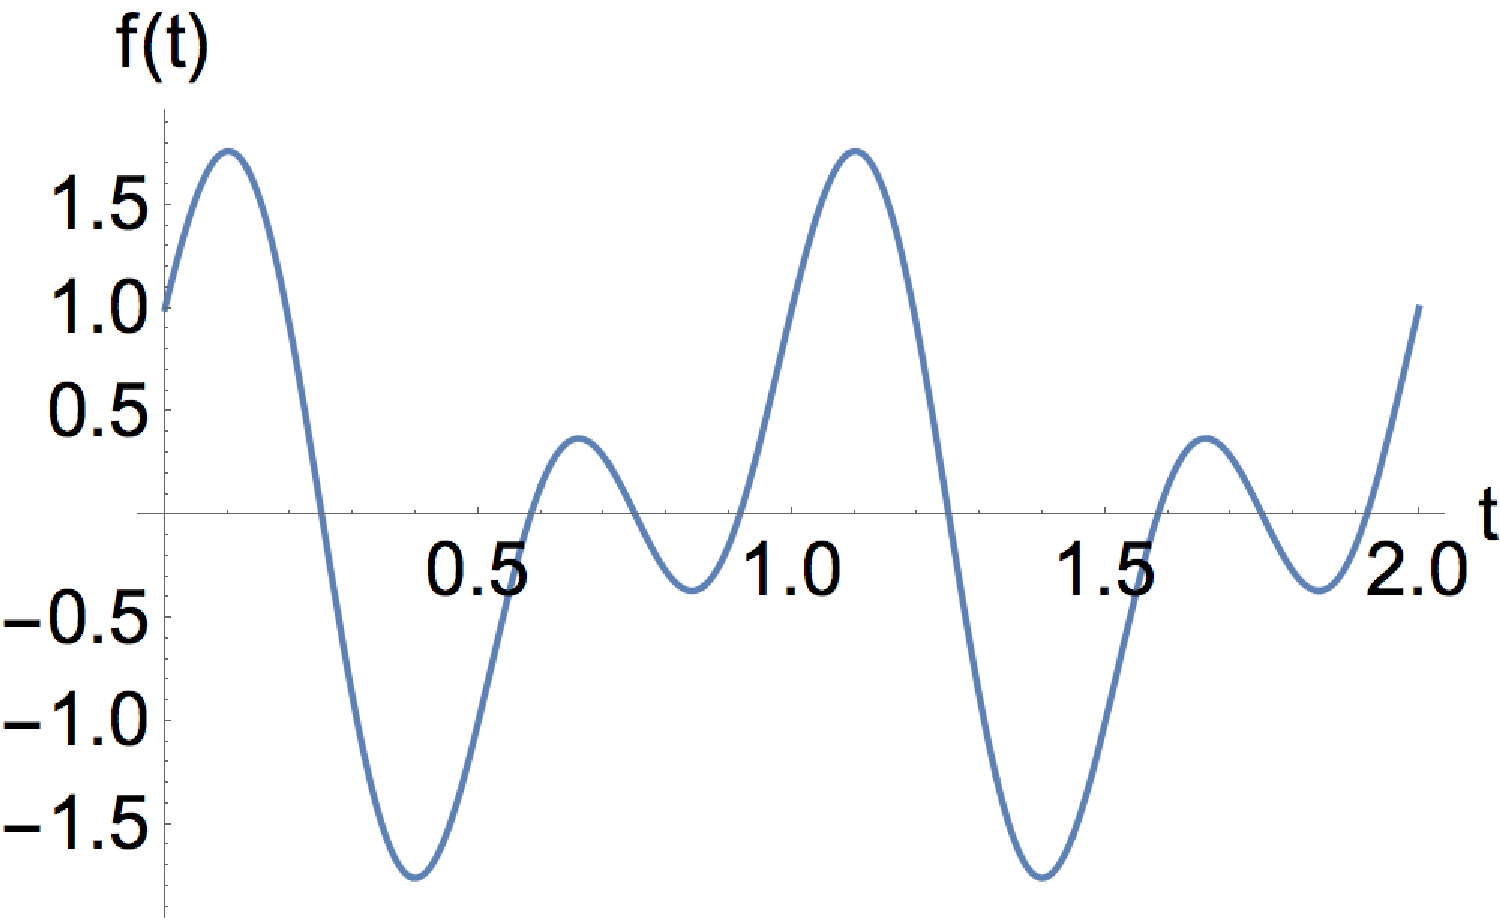
\includegraphics[scale=0.75]{dftcossin.png}

1. What are the two frequencies that make up the signal?

2. What is the fundamental frequency of this signal?

3. What is the maximum sampling frequency at which aliasing will occur for this signal?

\subsection*{Solutions}
\textbf{1.}\\
(Lower of the two frequencies in Hz)\\
\soltwodp{c}{166765}

(Higher of the two frequencies in Hz)\\
\soltwodp{d}{c22bee}

\textbf{2.}\\
(units: Hz)\\
\soltwodp{f}{6786da}

\textbf{3.}\\
(units: Hz)\\
\soltwodp{e}{0a9397}




%%%%%%%%%%%%%%%%%%%%%%%%%%%%%%%%%
\newpage
%%%%%%%%%%%%%%%%%%%%%%%%%%%%%%%%%
\section{Analysing a more complex function: part II}

\subsection*{Challenge}
Sampling the signal in the previous challenge 8 times per second:

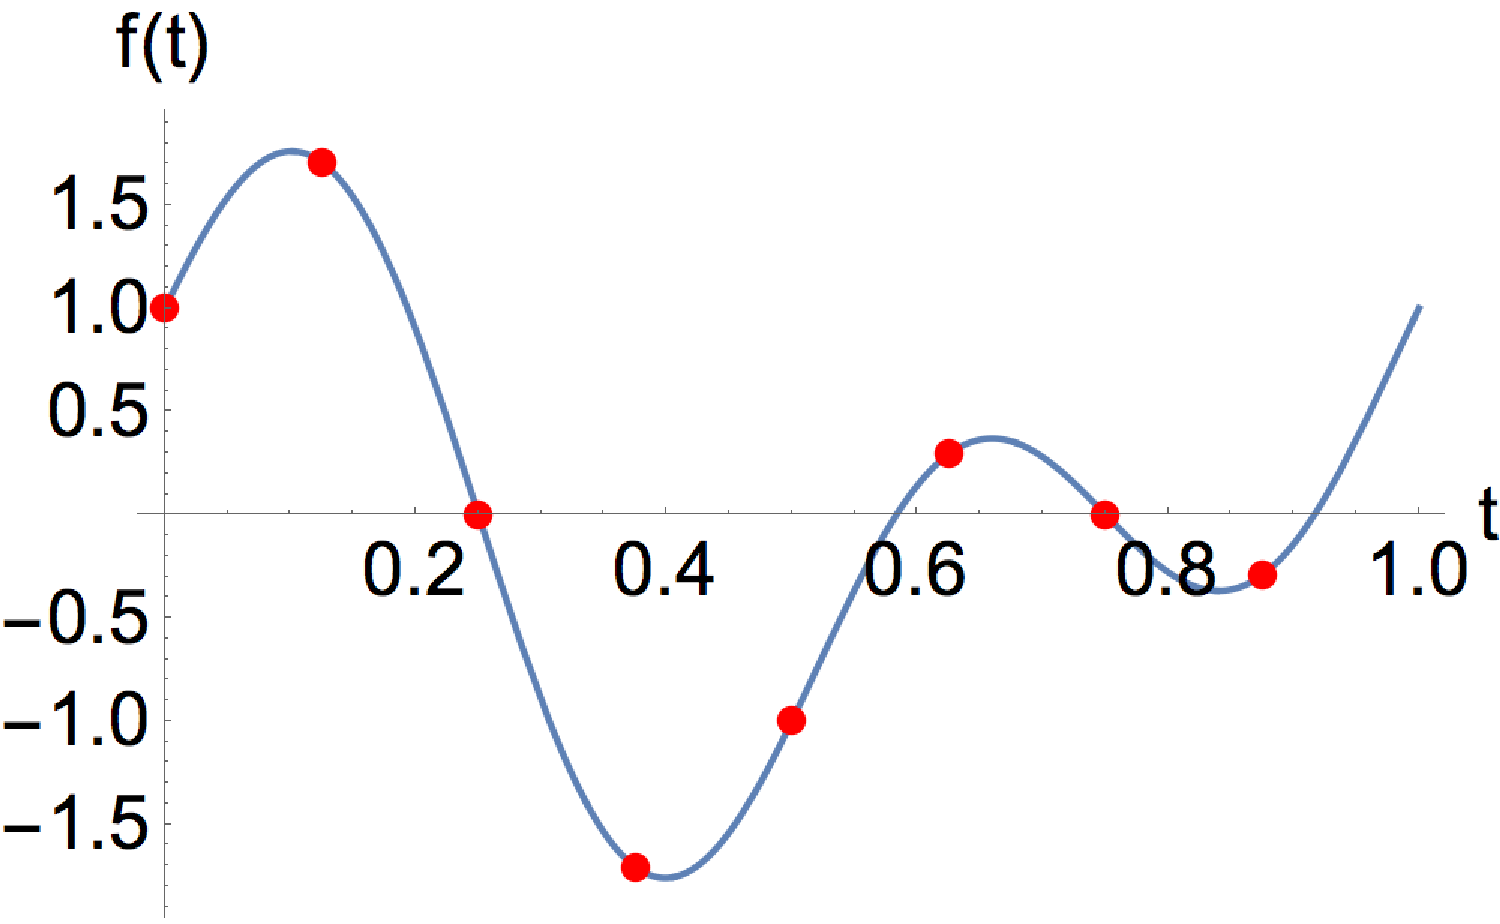
\includegraphics[scale=0.75]{dftcossinsamples.png}

yields values of
\begin{equation}
   \left(
\begin{array}{c}
 1. \\
 1.71 \\
 0. \\
 -1.71 \\
 -1. \\
 0.29 \\
 0. \\
 -0.29 \\
\end{array}
\right) 
\end{equation}

Calculating the matrix F yields

\begin{equation}
   \left(
\begin{array}{cccccccc}
 1 & 1              & 1 & 1 & 1 & 1 & 1 & 1 \\
 1 & (1-i)/\sqrt{2} & \bm{A} & -(1+i)/\sqrt{2} & -1 & (-1+i)/\sqrt{2} & i & (1+i)/\sqrt{2} \\
 1 & \bm{B}         & -1 & i & 1 & -i & -1 & i \\
 1 & -(1+i)/\sqrt{2}& i & (1-i)/\sqrt{2} & -1 & (1+i)/\sqrt{2} & -i & (-1+i)/\sqrt{2} \\
 1 & -1             & 1 & -1 & 1 & -1 & 1 & -1 \\
 1 & (-1+i)/\sqrt{2}& -i & (1+i)/\sqrt{2} & -1 & (1-i)/\sqrt{2} & i & -(1+i)/\sqrt{2} \\
 1 & i              & -1 & -i & 1 & i & -1 & -i \\
 1 & (1+i)/\sqrt{2} & i & (-1+i)/\sqrt{2} & -1 & -(1+i)/\sqrt{2} & -i & (1-i)/\sqrt{2} \\
\end{array}
\right) 
\end{equation}

1. Determine the missing values \textbf{A} and \textbf{B} by calculation.

2. Determine, by calculation, the frequencies with their magnitudes and phases of this signal. In this case, you can know the constituent frequencies, their magnitudes and phases because you know how the signal is made up of two signals. Check that your calculation aligns with your intuition.

\subsection*{Solutions}
\textbf{1. A}\\
\solimagtwodp{a}{223b8b}

\textbf{1. B}\\
\solimagtwodp{b}{df600a}

\textbf{2.} If you are not sure what your intuition should be, or if your answer does not match your intuition, please discuss with your partner or the teacher in class.


% NT: Go the other way to reconstruct a signal. Should spend an entire class on this.
%%%%%%%%%%%%%%%%%%%%%%%%%%%%%%%%%
\newpage
%%%%%%%%%%%%%%%%%%%%%%%%%%%%%%%%%
\section{The limits of DFT calculation}
\label{sec:dftlimits}

\subsection*{Resources}
Practically, the DFT is calculated using the Fast Fourier Transform (FFT). The reason is that the number of operations grows with the square of the number of samples which is unsustainable for typical signals.

The following pages are based on slides developed by Prof. Maraso Yamashiro for the 2015 class on Fourier Analysis, and highlight this problem quantitatively.

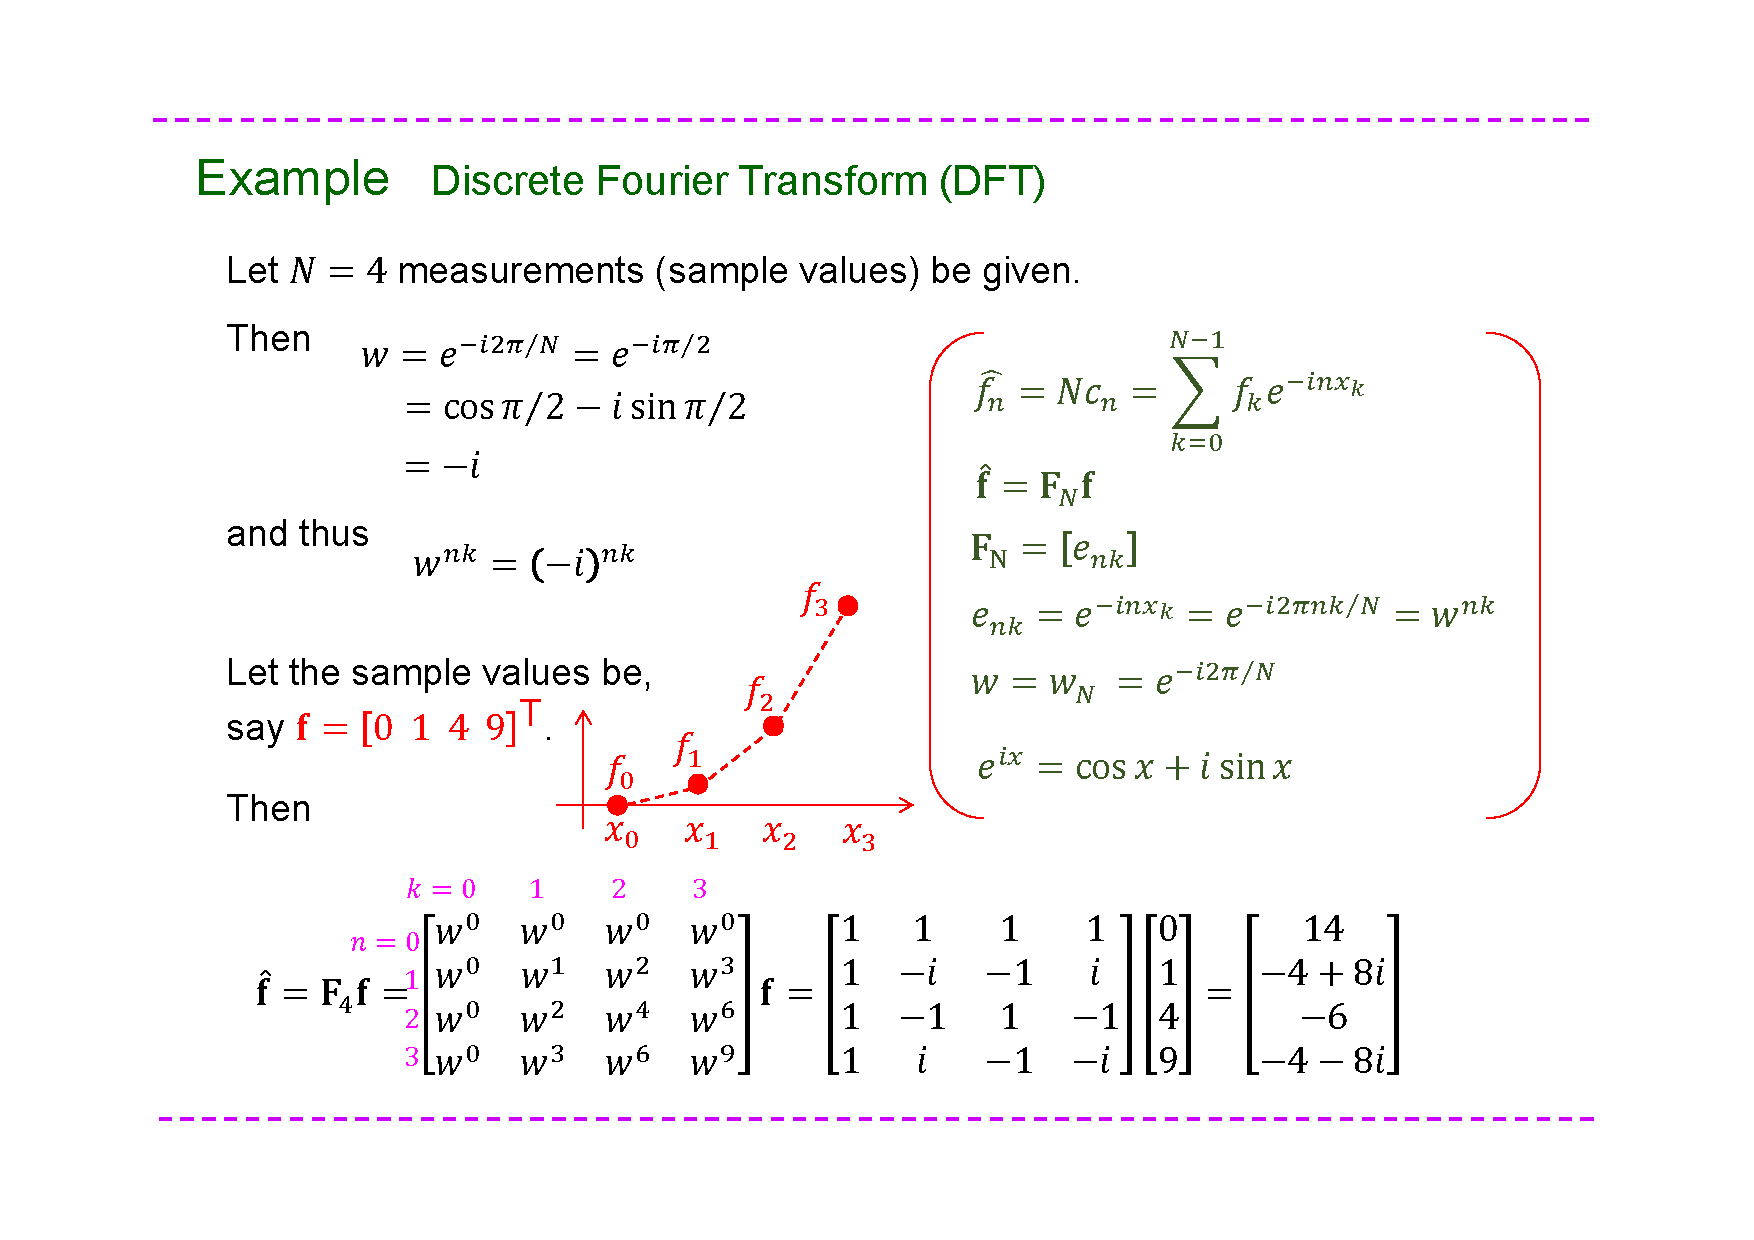
\includepdf[pages=-,pagecommand={},width=\textwidth,nup=1x2,frame=true]{fft_1-4.pdf}

\subsection*{Challenge}
Considering a signal sampled at 22 kHz, how many multiplications are required to calculate $F$ in the calculation $\bm{\hat{f}} = F \bm{f}$?

\subsection*{Solutions}
\solscitwodp{c}{eb9210}




%%%%%%%%%%%%%%%%%%%%%%%%%%%%%%%%%
\newpage
%%%%%%%%%%%%%%%%%%%%%%%%%%%%%%%%%
\section{The concepts of the FFT}

\subsection*{Resources}
The Cooley and Tukey algorithm for calculating the FFT is not that complicated, but can get very messy and it takes some time to really understand it. Therefore, we will limit ourselves to understanding some basic concepts upon which it is built.

The main concept is that many of the elements in the Fourier matrix are repetitive. For example, you can notice the symmetry about the diagonal in the $F_4$ matrix:

\begin{equation}
   F_4 = \left(
\begin{array}{cccc}
    1 & \tcr{1} & \tcr{1} & \tcr{1} \\
    \tcb{1} & -i & \tcr{-1} & \tcr{i} \\
    \tcb{1} & \tcb{-1} & 1 & \tcr{-1} \\
    \tcb{1} & \tcb{i} & \tcb{-1} & -i \\
\end{array}
\right) 
\end{equation}

One key concept therefore is that once we have calculated an element of the matrix, we don't need to calculate it again for elements that will turn out to be the same. The key question then becomes: how do we determine which elements will be repetitions of which other elements?

The ``twiddle factor'' shows how elements of matrix $F_N$ (ie, $w^{nk}$) are repeated. This can be visualised as points on a circle on the real-imaginary plane as the following slides from Prof. Maraso Yamashiro show.

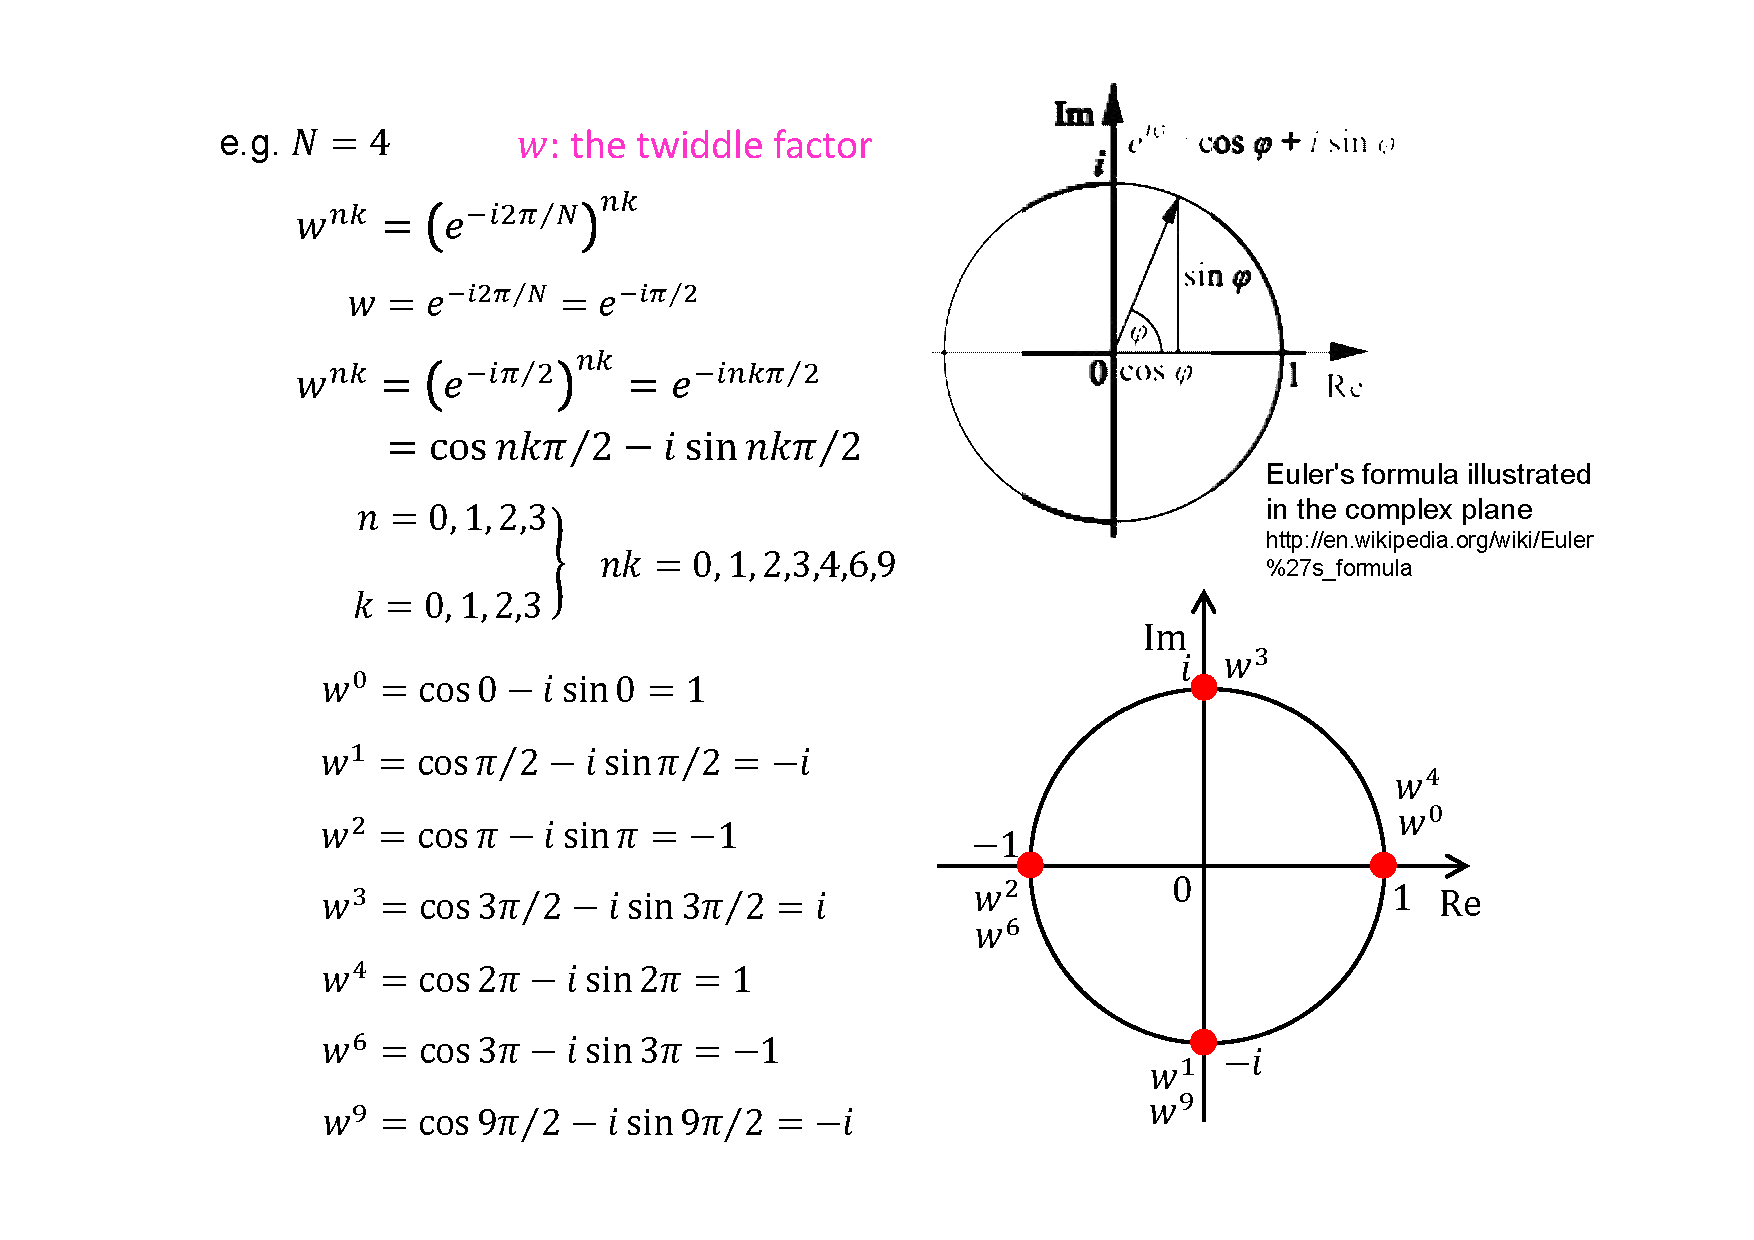
\includepdf[pages=-,pagecommand={},width=\textwidth,nup=1x2,frame=true]{fft_6-7.pdf}

First one can notice that repeated terms are consistently even or odd. For example, for $N=8$ it was seen that $w^0$, $w^8$, $w^{16}$ and $w^{24}$ all share the same value ($=1$) while $w_7$ and $w_{15}$ share the same (off-axis) value. You will notice however that simply breaking the functions into odd and even terms is not enough to unambiguously define the values of the twiddle factors, since even and odd terms can each still have multiple values.

One can take advantage of this symmetry (in ways not explained here) by taking the even-numbered terms and odd-numbered terms of the signal-vector $\bm{f}$ to create two new vectors, each of half the length of the original signal-vector:

\begin{align}
    \bm{f_{even}} &= [f_0, f_2, \dots, f_{N-2}]^T \\
    \bm{f_{odd}} &= [f_1, f_3, \dots, f_{N-1}]^T
\end{align}

Then renumbering the terms back to $0, 1, 2, \dots, N/2-1$:

\begin{align}
    \bm{f_{even}} &= [f_{ev,0}, f_{ev,1}, \dots, f_{ev,N/2-1}]^T \\
    \bm{f_{odd}} &= [f_{od,0}, f_{od,1}, \dots, f_{od,N/2-1}]^T \\
\end{align}

This can then be repeated, taking the even- and odd-numbered terms of $\bm{f_{even}}$ to make two more vectors of half-length, and doing the same for $\bm{f_{odd}}$ so we now have 4 vectors each $1/4$ the length of the original signal-vector $\bm{f}$. This is repeated until there are $N/2$ vectors each of length $2$.

Although beyond the scope of the explanation here, this ultimately allows one to take advantage of the repetitive nature of the twiddle factor, reducing the scaling of the number of multiplications drastically from $N^2$ to $Nlog_2 N$, as shown in the following slide from Prof. Maraso Yamashiro:

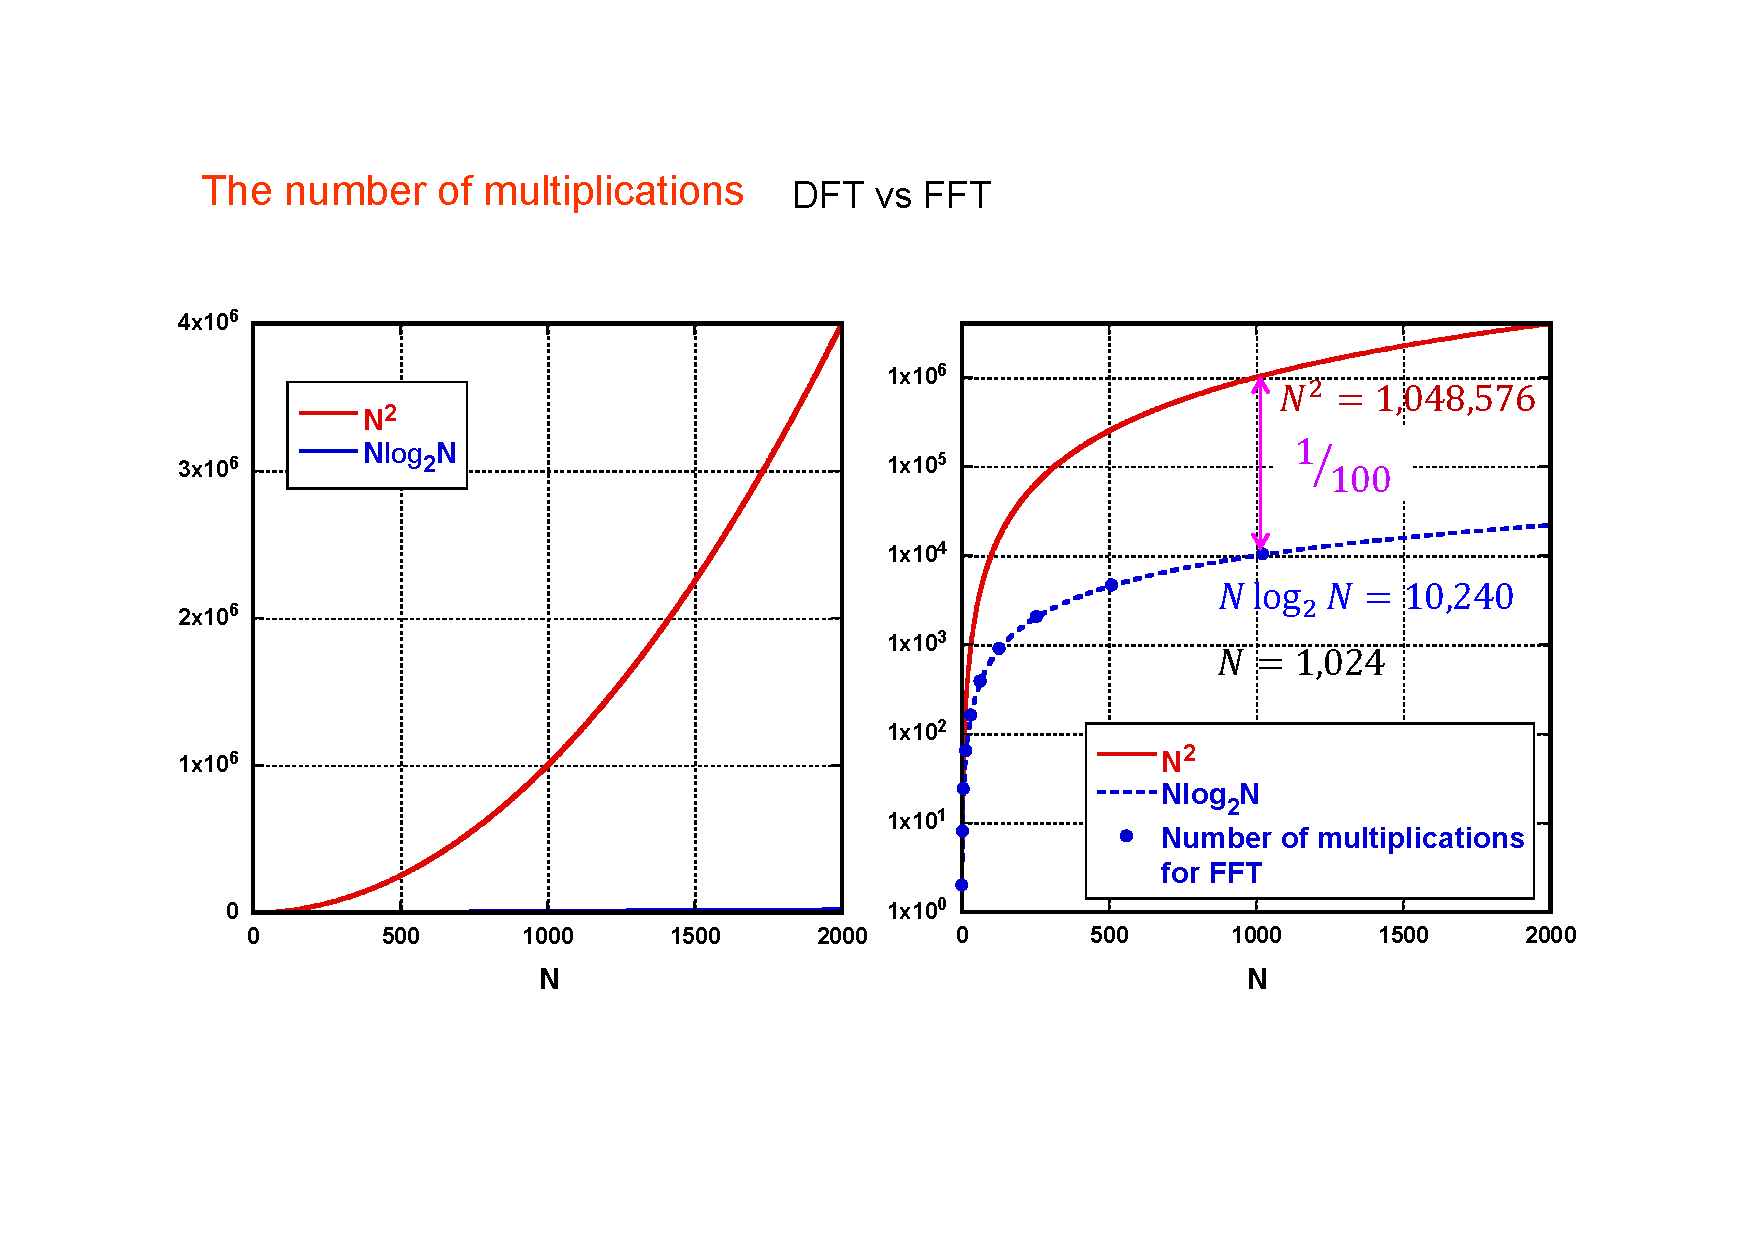
\includepdf[pages=-,pagecommand={},width=\textwidth,nup=1x2,frame=true]{fft_28.pdf}

A further point to note is that, in order to continuously divide the signal in half until each vector is length $2$, the original signal must be of length $2^p$ where p is some integer. For example, a signal of length $8$ such as $\bm{[1,2,3,4,5,6,7,8]}$ can be halved once into two vectors of length four ($\bm{[1,3,5,7]}$ and $\bm{[2,4,6,8]}$) and then again into four vectors of length two ($\bm{[1,5]}$, $\bm{[3,7]}$, $\bm{[2,6]}$, $\bm{[4,8]}$). If the vector is of length 9 however, such as $\bm{[1,2,3,4,5,6,7,8,9]}$, the signal cannot be divided into two signals of \emph{equal length}.

This problem is overcome through the use of \emph{zero-padding}. In the example in the previous paragraph, the signal of length $9$ would simply have seven zeros added to it at the end to create a signal of total length $16$ ($\bm{[1,2,3,4,5,6,7,8,9,0,0,0,0,0,0,0]}$), which could then be halved three times into eight vectors of length $2$.

\subsection*{Challenge}
1. Considering the signal that generated the spectrum in challenge \ref{sec:dftlimits}, how many zeros must be added to the end of the sampled signal to permit FFT to be performed?

2. How many times can the padded signal be halved?

3. How many multiplications does this signal require under FFT?

4. Considering the original unpadded signal, how many times more multiplications are required under standard DFT compared to processing under FFT?

\subsection*{Solutions}
\textbf{1}\\
\solscitwodp{d}{293b72}

\textbf{2}\\
\soltwodp{e}{f5df85}

\textbf{3}\\
491,520

\textbf{4}\\
984.70




%%%%%%%%%%%%%%%%%%%%%%%%%%%%%%%%%
\newpage
%%%%%%%%%%%%%%%%%%%%%%%%%%%%%%%%%
\section{Signal processing with Python}

\subsection*{Comment}
Here you can put your understanding to practical use by cleaning the noise from an audio signal. This gives you experience of a very common application of Fourier analysis.

Note that running the python program will result in sound being played, which can be loud. PLEASE BE VERY CAREFUL WHEN PLAYING THE SOUND FOR THE FIRST TIME, ESPECIALLY IF YOU ARE WEARING HEADPHONES.

Graphs will also be displayed in the default browser on your computer.

For Mac users: I recommend downloading the terminal software iTerm2 (\url{https://www.iterm2.com}). It is much easier to use than the default terminal on Macs.

When you download the files below, I recommend that you create a new directory beforehand (for example, on your desktop) and save all the files to that new directory.

\subsection*{Resources}
\begin{itemize}
    \item Python outline code: \url{http://raw.githubusercontent.com/NanoScaleDesign/FourierAnalysis/master/Audio/audio.py} *
    \item Noisy audio (to be read by the python code): \url{http://raw.githubusercontent.com/NanoScaleDesign/FourierAnalysis/master/Audio/bbcnews181210.noisy.wav} *
    \item Noisy audio (media-player format**): \url{http://raw.githubusercontent.com/NanoScaleDesign/FourierAnalysis/master/Audio/bbcnews181210.mediaformat.noisy.wav}
\end{itemize}

* If this brings up a webpage, you might need to right-click on the page and download it, ensuring the name is correct.\\
** Can be played in a media player such as iTunes or VLC.

\subsection*{Challenge}
You are trying to listen to the BBC news but there is background noise that makes it difficult to hear. Your challenge is to remove the noise from the signal.

You may use the outline python code above to help you, or you may use your own code from scratch. The code above relies on the following libraries:
\begin{itemize}
    \item sounddevice
    \item numpy
    \item scipy
    \item plotly
\end{itemize}

Generally, to install new libraries you can use \emph{pip3 install sounddevice} etc.

\subsection*{Solutions}
There will be a final output file called \emph{bbcnews181210.mediaformat.clean.wav}.
You can play this in a media player such as iTunes or VLC, and should be a clean sound without the background noise.




%%%%%%%%%%%%%%%%%%%%%%%%%%%%%%%%%
\newpage
%%%%%%%%%%%%%%%%%%%%%%%%%%%%%%%%%
\section{2D Fourier Transform}

\subsection*{Comment}
2D fourier transforms primarily come up in relation to images. The extention from 1D to 2D is fairly straightforward, and this challenge is designed to give you a basic understanding of the transition to multiple dimensions.

Note: Discrete-Time Fourier Transforms are mentioned briefly in the video resource below. This is not something we have time to cover in this course so you may ignore that part of the video. Also, we have not really discussed the inverse DFT and we will not cover this in this course apart from a programming perspective.

\subsection*{Resources}
\begin{itemize}
    \item Video: \url{https://youtu.be/NbQY1x8H6QQ?t=137} from 2:17 until 18:25.
\end{itemize}

\subsection*{Challenge}
1. Relate the 2D Discrete Fourier Transform shown in the video to the 1D DFT you are already familiar with. What has changed?

2. What is meant by a two-dimensional basis function? Draw an example of a 2D basis function and describe its relation to the 2D DFT.

\subsection*{Solution}
Please compare your solutions with your partner and discuss in class.




%%%%%%%%%%%%%%%%%%%%%%%%%%%%%%%%%
\newpage
%%%%%%%%%%%%%%%%%%%%%%%%%%%%%%%%%
\section{Edge detection and blurring with Fourier analysis and Python}

\subsection*{Comment}
In the 1D case, after performing DFT, low frequencies are considered to be on the left and high frequencies on the right.
In 2D, the low frequencies are considered to be in the top-left corner.
Due to symmetry however, modification of frequencies typically requires both altering the intended frequency as well as its symmetrical counterpart.
As a consequence, the spectrum in 2D is usually shifted so that the lowest frequencies are in the centre of the image. This is done using the \emph{fftshift} function of numpy.

\subsection*{Resources}
\begin{itemize}
    \item Python outline code: \url{http://raw.githubusercontent.com/NanoScaleDesign/FourierAnalysis/master/Image_processing/image_processing.py}
    \item Kyudai image: \url{http://raw.githubusercontent.com/NanoScaleDesign/FourierAnalysis/master/image_processing/kyudai.png}
\end{itemize}

\subsection*{Challenge}
Here you are going to use your Fourier Analysis knowledge and python skills to do image-processing.

\begin{enumerate}
    \item Convert the original image of the Kyudai logo so that only the edges of the image are shown.
    \item Convert the original image of the Kyudai logo so that the image becomes blurred.
    \item \label{it:reasoning} Write a paragraph summarising the reasoning of your approach.
    \item \label{it:extraimage} (optional) Try with another image (requirements for pre-processing the image can be found in the python file above).
\end{enumerate}

You may use the outline python code above to help you, or you may use your own code from scratch. The code above relies on the following libraries:
\begin{itemize}
    \item numpy
    \item PIL
\end{itemize}

Generally, to install new libraries you can use \emph{pip3 install numpy} etc.

The code above will output the shifted DFT of the image to \emph{kyudai.fft.png} and the inverse DFT of the image to \emph{kyudai.fft.ifft.png}.


\includegraphics[width=5cm]{kyudai.png}

\includegraphics[width=5cm]{kyudai_outline.png}

\includegraphics[width=5cm]{kyudai_blurred.png}

\emph{Original image} ~ ~ ~ ~ ~ ~ ~ ~ ~ ~ ~ ~
\emph{Edge-only image} ~ ~ ~ ~ ~ ~ ~ ~ ~ ~
\emph{Blurred image}

\subsection*{Solutions}
You should be able to generate images that are similar to those shown above. Please compare your answer for part (\ref{it:reasoning}) with your partner and consider sharing any interesting images generated in part (\ref{it:extraimage}) with others in the class!

%\appendix 
%\chapter{Practise challenges}
%%%%%%%%%%%%%%%%%%%%%%%%%%%%%%%%%%
\newpage
%%%%%%%%%%%%%%%%%%%%%%%%%%%%%%%%%
\section{Shifting squarewave} 

\subsection*{Challenge}
Determine the Fourier series in terms of exponentials and trigonometric terms for the square-wave below and compare it to the square-wave you calculated earlier in challenge \ref{sec:fs_squarewave}. Notice how the presence of the terms are related to the even/odd nature of the function.

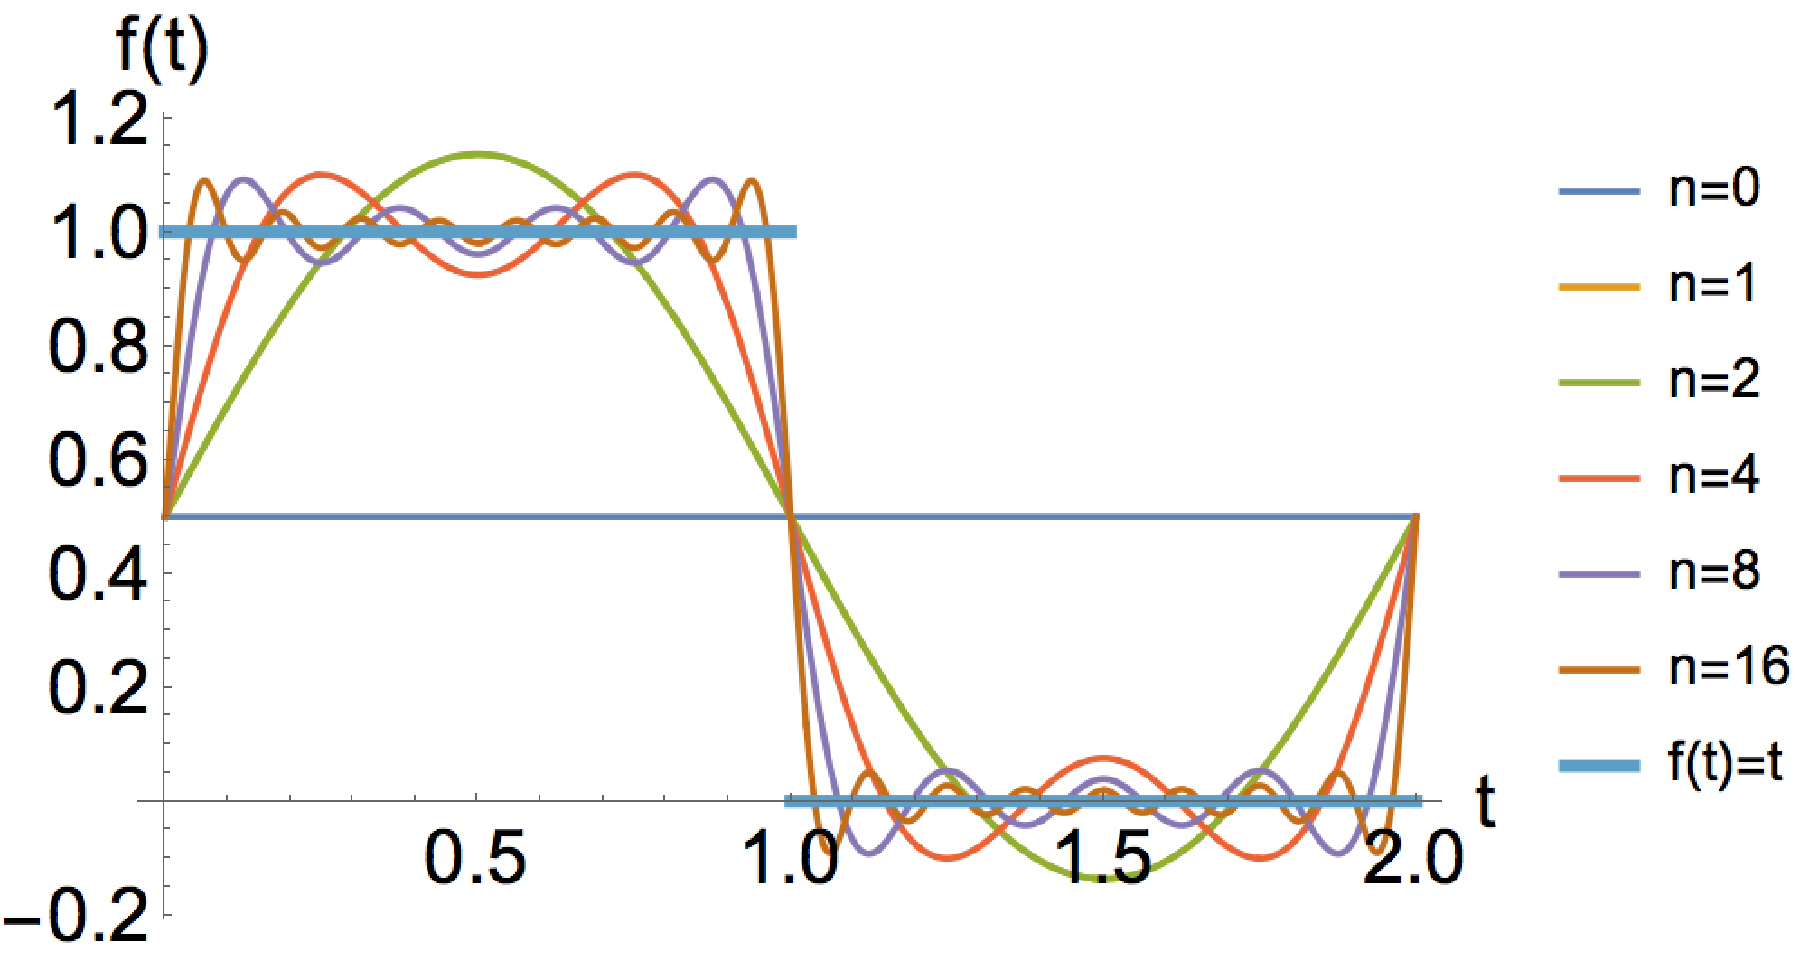
\includegraphics{fs_square_wave_II.png}




%%%%%%%%%%%%%%%%%%%%%%%%%%%%%%%%%
\newpage
%%%%%%%%%%%%%%%%%%%%%%%%%%%%%%%%%
\section{Sawtooth wave} 
\label{sec:sawtooth}

\subsection*{Challenge}
1. Determine the expression for a sawtooth wave of the form shown in the graph below, in terms of a trigonometric Fourier series.

2. Write a sentence explaining how the symmetry of the problem effects the final expression.

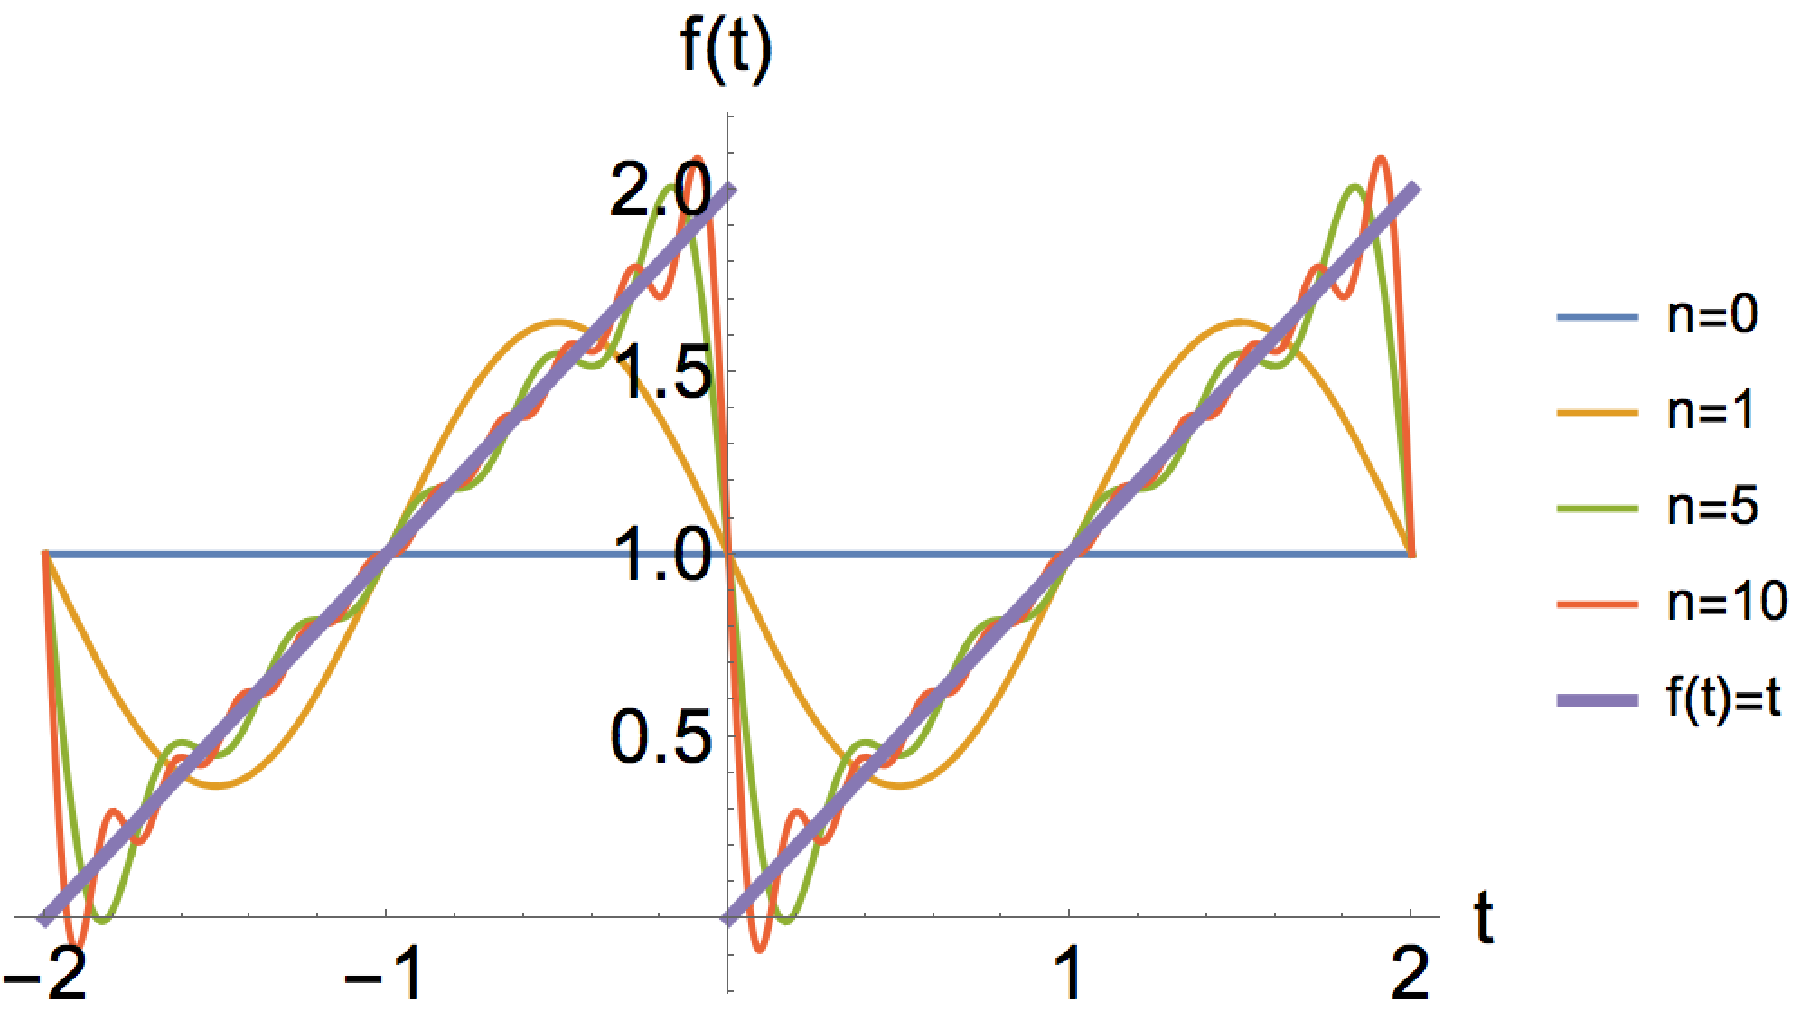
\includegraphics{fs_sawtooth_wave.png}

To check your answer, evaluate the function at $t=1.1$ including only the first 3 terms of the Fourier series.

\subsection*{Solution}
\hash{apaa}{603043}

%\chapter{Mid-term exam questions}
%\section{}

What are the Fourier coefficients $C_{-1}$, $C_{0}$ and $C_{1}$ of the exponential Fourier series for the function below?

\begin{equation}
  f(x)=2+cos(2 \pi x)
\end{equation}




\section{}

Considering the periodic squarewave described by the function

\begin{equation}
    f(t)=
    \begin{cases}
        0 & \text{for } 0<t<1 \\
        -1 & \text{for } 1<t<2
    \end{cases}
\end{equation}

\begin{center}
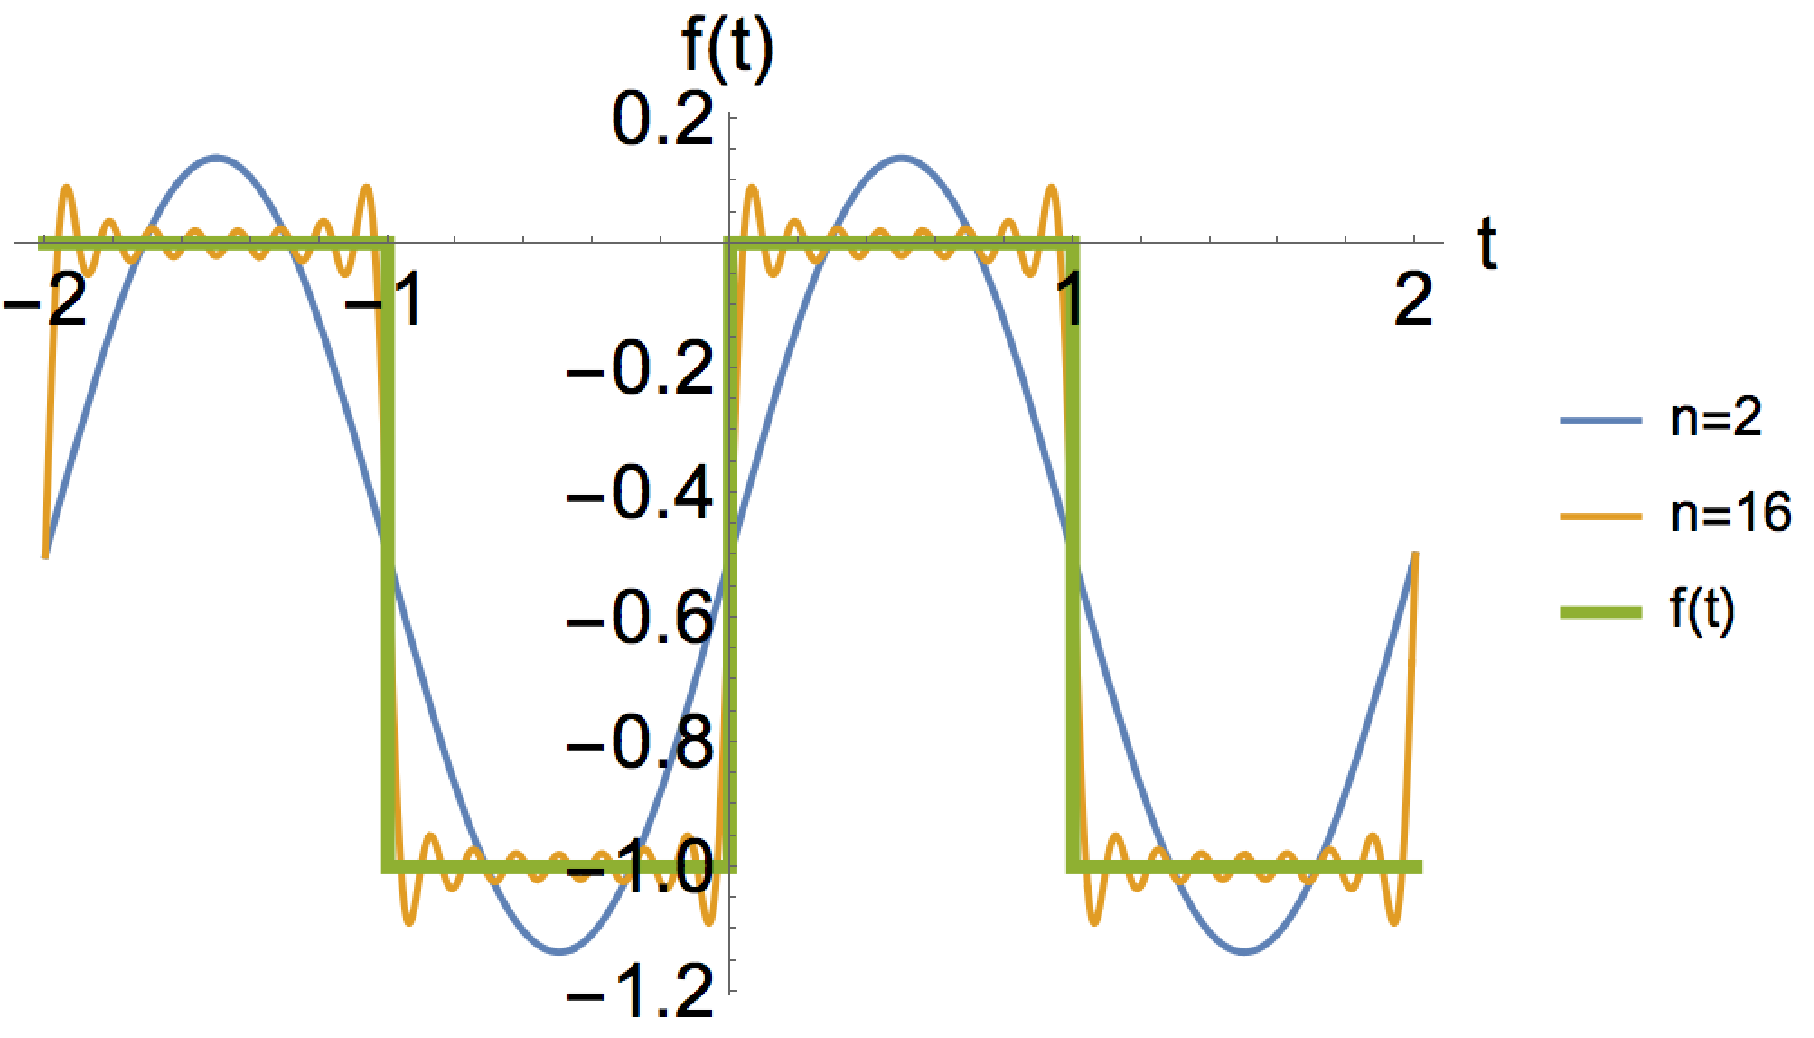
\includegraphics[scale=0.75]{fourier_series_square_wave_midtermexam.png}
\end{center}

1. Calculate the Fourier coefficient $C_0$.

2. Obtain an expression for the Fourier coefficients $C_k$ where $k \ne 0$. Write your final answer so that it does not contain any exponentials, sines or cosines.

3. What is Gibb's phenomenon? Under what situations does it occur?




\section{}

In the first lecture we saw that it was possible to make any function (such as the ``Homer Simpson'' function) by taking a point and rotating it around a circle that itself was rotating around a larger circle, that itself was rotating around a larger circle, and so on. This is also how the ancient greeks tried to approximate the orbit of the planets and sun around the earth.

1. How is the ability to approximate an arbitrary function using sums of circles related to Fourier series? You may refer to the equation
\begin{equation}
    f(t) = \sum_{k=-N}^{k=N} C_k e^{2 \pi i k t}
\end{equation}
during your discussion.

2. By what variables are frequencies and radii of the circles defined in the Fourier series in the above equation?

3. The terms of the Fourier series are orthogonal. Describe in a few sentences what this means. You may refer to the below expression in your answer.
\begin{equation}
    (e^{2 \pi i k_1 t},e^{2 \pi i k_2 t})
\end{equation}

\end{document}
